\documentclass[a4paper, pdf, twoside]{book}
\usepackage{iesbbook}
\geometry{a4paper,total={170mm,257mm},left=30mm,right=23mm,top=35mm,bottom=30mm,headsep=35pt}
\begin{document}
\thispagestyle{empty}
\pagestyle{plain}
\renewcommand{\headrulewidth}{0pt}
\begin{center}
\vspace*{0.5cm}\hrule\vspace{0.5cm}
\Huge \textbf{Matemàtiques I} \par
\Large 1r de Batxillerat de ciències\par
\large \textit{Sèrie Pràctica}\par
\vspace{0.5cm}\hrule\vspace{0.5cm}
\Huge \textbf{\textsc{Solucionari}} \par \vspace{1.5cm}
	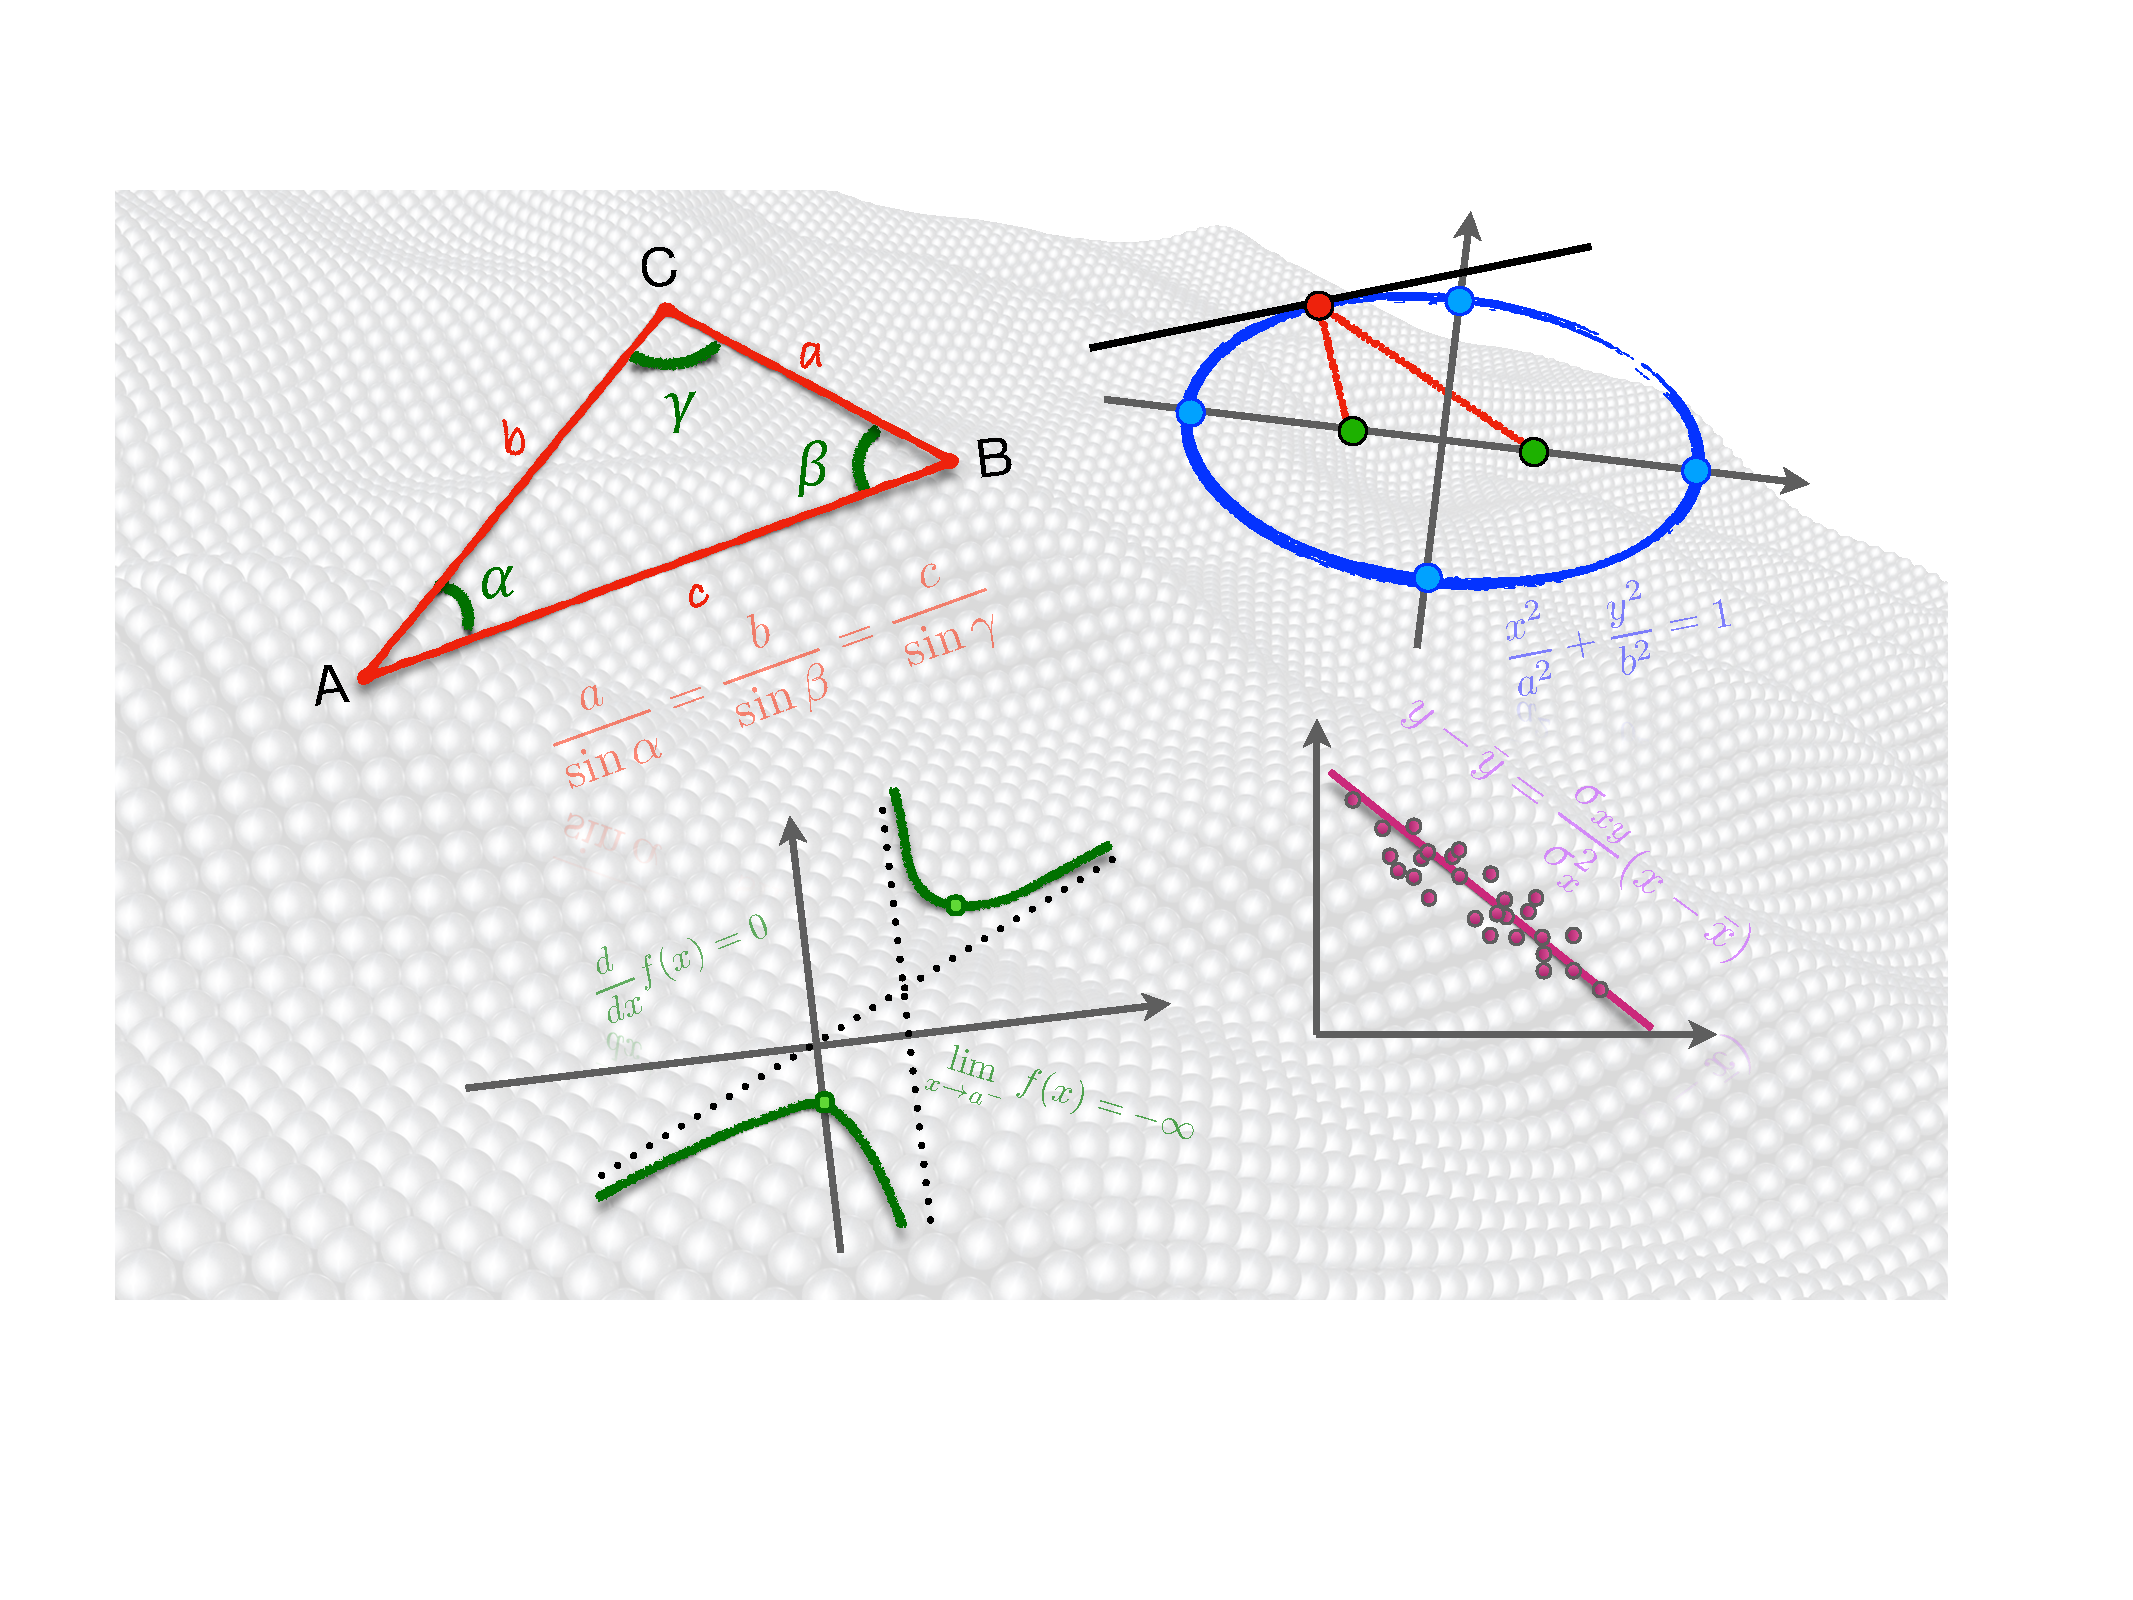
\includegraphics[width=0.9\textwidth]{img-00/portada}   

	\vspace{1.5cm}  
	\begin{minipage}{0.4\textwidth}  
		\begin{center}  
			\includegraphics*[width=1.2in]{img-00/ies-binissalem-logo}  
			\small  
			\noindent \href{www.iesbinissalem.net}{\textbf{www.iesbinissalem.net}}  
		\end{center}  
	\end{minipage}  
	\begin{minipage}{0.4\textwidth}  
		\begin{flushright}  
			\normalsize \textbf{Josep Mulet}\par 
			\textit{Departament de Matemàtiques}\par   
			IES Binissalem  
		\end{flushright}  
	\end{minipage}   
	\end{center}   
\cleartorightpage
\renewcommand{\baselinestretch}{1.5}
\tableofcontents \cleartorightpage
\renewcommand{\baselinestretch}{1}
\def\currentname{}
\pagestyle{fancy}
\renewcommand{\headrulewidth}{0.5pt}
\fancyhead[LE,RO]{\large\textcolor{darkBlueColor}{\shadowbox{\fontfamily{phv}\selectfont\textbf{\, \thepage \,}}}}
\fancyhead[LO,RE]{{ \fontfamily{phv}\selectfont \textit{\currentname} }}
\fancyfoot{}
\fontsize{10.5}{12}\selectfont
\begin{multicols}{2}
\def\currentname{Solucions del Tema 1}
\vspace*{0.75cm}

 
 \needspace{5\baselineskip} 
 \scalebox{1.25}{\heading{Solucions del Tema 1}}

\vspace*{0.4cm}
\phantomsection \addcontentsline{toc}{section}{Solucions del Tema 1}
\vspace{0.3cm}

 \needspace{4\baselineskip} 

{\textbf{\em Pàgina 10}} \hrulefill
\begin{enumerate}
\vspace{0.25cm}


 \needspace{2\baselineskip} 

 \item[\fontfamily{phv}\selectfont\color{blue}\textbf{1}. ] 
 \begin{tasks}[column-sep=1em, item-indent=1.3333em](2)
	 \task $0.\hat 6$
	 \task $0.75$
	 \task $0.2\hat 3$
	 \task $0.24$
	 \task $0.875$
	 \task $0.\widehat {81}$
\end{tasks}
 \end{enumerate}
\begin{enumerate}
\vspace{0.25cm}


 \needspace{2\baselineskip} 

 \item[\fontfamily{phv}\selectfont\color{blue}\textbf{2}. ] 
 \begin{tasks}[column-sep=1em, item-indent=1.3333em](2)
	 \task $233/99$
	 \task $431821/3300$
	 \task $1$
\end{tasks}
 \end{enumerate}
\vspace{0.3cm}

 \needspace{4\baselineskip} 

{\textbf{\em Pàgina 11}} \hrulefill
\begin{enumerate}
\vspace{0.25cm}


 \needspace{2\baselineskip} 

 \item[\fontfamily{phv}\selectfont\color{blue}\textbf{5}. ] 
 \begin{tasks}[column-sep=1em, item-indent=1.3333em](3)
	 \task 5
	 \task 5
	 \task $\sqrt {10}-\pi $
\end{tasks}
 \end{enumerate}
\begin{enumerate}
\vspace{0.25cm}


 \needspace{2\baselineskip} 

 \item[\fontfamily{phv}\selectfont\color{blue}\textbf{6}. ] 
 \begin{tasks}[column-sep=1em, item-indent=1.3333em](2)
	 \task 4
	 \task 2.2
	 \task 2
	 \task 9
\end{tasks}
\vspace{0.25cm}


 \needspace{2\baselineskip} 

 \item[\fontfamily{phv}\selectfont\color{blue}\textbf{7}. ] 
 \begin{tasks}[column-sep=1em, item-indent=1.3333em](2)
	 \task $1\leq x<7$
	 \task $-3<x<5$
	 \task $2<x\leq 8$
	 \task $x<6$
\end{tasks}
\vspace{0.25cm}


 \needspace{2\baselineskip} 

 \item[\fontfamily{phv}\selectfont\color{blue}\textbf{8}. ] 
 \begin{tasks}[column-sep=1em, item-indent=1.3333em](2)
	 \task $(2,5)$
	 \task $(4,+\infty )$
	 \task $[3,6)$
	 \task $(-\infty ,7]$
\end{tasks}
\vspace{0.25cm}


 \needspace{2\baselineskip} 

 \item[\fontfamily{phv}\selectfont\color{blue}\textbf{9}. ] 
 \begin{tasks}[column-sep=1em, item-indent=1.3333em](2)
	 \task $(26,100]$
	 \task $[0,18]$
	 \task $(2,+\infty )$
	 \task $[100,1000)$
	 \task $(-\infty ,25)$
	 \task $[0,+\infty )$
	 \task $(1,9)$
\end{tasks}
 \end{enumerate}
\vspace{0.3cm}

 \needspace{4\baselineskip} 

{\textbf{\em Pàgina 12}} \hrulefill
\begin{enumerate}
\vspace{0.25cm}


 \needspace{2\baselineskip} 

 \item[\fontfamily{phv}\selectfont\color{blue}\textbf{10}. ] 
 \begin{tasks}[column-sep=1em, item-indent=1.3333em](2)
	 \task $(-4,6)$
	 \task $(-14/3,2/3)$
	 \task $(-10.001,-9.999)$
\end{tasks}
 \end{enumerate}
\begin{enumerate}
\vspace{0.25cm}


 \needspace{2\baselineskip} 

 \item[\fontfamily{phv}\selectfont\color{blue}\textbf{11}. ] 
 \begin{tasks}[column-sep=1em, item-indent=1.3333em](2)
	 \task $(5.5,1.5)$
	 \task $(-5.5,1.5)$
	 \task $(-0.5,2.5)$
\end{tasks}
\vspace{0.25cm}


 \needspace{2\baselineskip} 

 \item[\fontfamily{phv}\selectfont\color{blue}\textbf{12}. ] 
 \begin{tasks}[column-sep=1em, item-indent=1.3333em](2)
	 \task $x=$ 5 i --5
	 \task $x=$ 4
	 \task $x=$ --10 i 4
\end{tasks}
\vspace{0.25cm}


 \needspace{2\baselineskip} 

 \item[\fontfamily{phv}\selectfont\color{blue}\textbf{13}. ] 
 \begin{tasks}[column-sep=1em, item-indent=1.3333em](1)
	 \task $(-1,1)$
	 \task* $(-\infty ,-1]\cup [1,+\infty ]$
	 \task* $(-\infty ,2)\cup (4,+\infty )$
	 \task* $(-\infty ,2]\cup [4,+\infty )$
\end{tasks}
\vspace{0.25cm}
\item[\fontfamily{phv}\selectfont\color{blue}\textbf{14. }] 
$-3$ i $9$. $-5.5$ i $1.5$. $9-(-5.5)=14.5$
\vspace{0.25cm}
\item[\fontfamily{phv}\selectfont\color{blue}\textbf{15. }] 
$[-3, 8)$
\vspace{0.25cm}
\item[\fontfamily{phv}\selectfont\color{blue}\textbf{16. }] 
$[5,11]$
\vspace{0.25cm}


 \needspace{2\baselineskip} 

 \item[\fontfamily{phv}\selectfont\color{blue}\textbf{17}. ] 
 \begin{tasks}[column-sep=1em, item-indent=1.3333em](2)
	 \task* $A\cap B=\emptyset $;\par $A\cup B=[-11,-9] \cup (-1,6)$;\par $A-B=A$
	 \task* $A\cap B=B$; $A\cup B=A$;\par $A-B=[-5,3]\cup [4,5]$
\end{tasks}
\vspace{0.25cm}


 \needspace{2\baselineskip} 

 \item[\fontfamily{phv}\selectfont\color{blue}\textbf{18}. ]  \scalebox{0.6}{\simbolclau } 
 \begin{tasks}[column-sep=1em, item-indent=1.3333em](3)
	 \task $\sqrt [{6}]{5} $
	 \task $\sqrt [{8}]{8} $
	 \task $\sqrt [{8}]{x^{7} } $
\end{tasks}
\vspace{0.25cm}


 \needspace{2\baselineskip} 

 \item[\fontfamily{phv}\selectfont\color{blue}\textbf{19}. ]  \scalebox{0.6}{\simbolclau } 
 \begin{tasks}[column-sep=1em, item-indent=1.3333em](2)
	 \task $2\,\sqrt [{}]{2} $
	 \task $9\,\sqrt [{}]{3} $
	 \task $\sqrt [{3}]{6} $
	 \task $2\,\sqrt [{4}]{2} $
	 \task $\sqrt [{3}]{3} $
	 \task $\sqrt [{3}]{49} $
	 \task $\sqrt [{8}]{7} $
	 \task $\sqrt {2} $
\end{tasks}
\vspace{0.25cm}


 \needspace{2\baselineskip} 

 \item[\fontfamily{phv}\selectfont\color{blue}\textbf{20}. ]  \scalebox{0.6}{\simbolclau } 
 \begin{tasks}[column-sep=1em, item-indent=1.3333em](2)
	 \task* $\sqrt [{4}]{2^{3} } =\sqrt [{12}]{2^{9} } $
	 \task* $\sqrt {7} =\sqrt [{16}]{7^{8} } $
	 \task* $\sqrt [{4}]{a^{6} } =\sqrt {a^{3} } $
	 \task* $\sqrt [{6}]{5^{12} } =\sqrt [{3}]{5^{6} } =5^{2} $
\end{tasks}
 \end{enumerate}
\vspace{0.3cm}

 \needspace{4\baselineskip} 

{\textbf{\em Pàgina 13}} \hrulefill
\begin{enumerate}
\vspace{0.25cm}


 \needspace{2\baselineskip} 

 \item[\fontfamily{phv}\selectfont\color{blue}\textbf{21}. ]  \scalebox{0.6}{\simbolclau } 
 \begin{tasks}[column-sep=1em, item-indent=1.3333em](2)
	 \task $\sqrt [{3}]{5/4} $
	 \task $\sqrt [{12}]{2^{3} \cdot 3} $
	 \task $\sqrt [{12}]{5^{7} } $
	 \task $2^{3} $
	 \task $2^{4} \cdot \sqrt [{5}]{2^{4} } $
	 \task $\sqrt [{}]{5} $
	 \task 3
	 \task $5^{2} $
\end{tasks}
 \end{enumerate}
\begin{enumerate}
\vspace{0.25cm}


 \needspace{2\baselineskip} 

 \item[\fontfamily{phv}\selectfont\color{blue}\textbf{22}. ]  \scalebox{0.6}{\simbolclau } 
 \begin{tasks}[column-sep=1em, item-indent=1.3333em](2)
	 \task  $15\,\sqrt [{}]{11} $
	 \task $6\,\sqrt [{3}]{2} $
	 \task $-\sqrt [{}]{6} /5$
	 \task $-14\,\sqrt [{4}]{2} /3$
	 \task $41\,\sqrt [{}]{3} /15$
	 \task $13\,\sqrt [{}]{2} /5$
\end{tasks}
\vspace{0.25cm}
\item[\fontfamily{phv}\selectfont\color{blue}\textbf{23. }]  \scalebox{0.6}{\simbolclau } 
$(2+a)^{2} +4(2+a)\sqrt {a} +4a$
\vspace{0.25cm}


 \needspace{2\baselineskip} 

 \item[\fontfamily{phv}\selectfont\color{blue}\textbf{24}. ]  \scalebox{0.6}{\simbolclau } 
 \begin{tasks}[column-sep=1em, item-indent=1.3333em](2)
	 \task $\frac {\sqrt [{3}]{3^{2} } }{3} $
	 \task $\frac {3}{4} \,\sqrt [{4}]{2^{3} }$
	 \task $3(\sqrt {2+1} )$
	 \task $3+2\sqrt {2} $
	 \task $(\sqrt {10} -\sqrt {6} )/2$
	 \task $-(9+4\sqrt {5} )$
\end{tasks}
\vspace{0.25cm}


 \needspace{2\baselineskip} 

 \item[\fontfamily{phv}\selectfont\color{blue}\textbf{25}. ]  \scalebox{0.6}{\simbolclau } 
 \begin{tasks}[column-sep=1em, item-indent=1.3333em](2)
	 \task $3\sqrt {6}$
	 \task* $\frac {\sqrt [{4}]{2^{3} } }{2} $
	 \task $\frac {\sqrt {3} }{2} $
	 \task 35
	 \task $2^{-64/15} $
	 \task $33/4-5\sqrt {2} $
\end{tasks}
 \end{enumerate}
\vspace{0.3cm}

 \needspace{4\baselineskip} 

{\textbf{\em Pàgina 14}} \hrulefill
\begin{enumerate}
\vspace{0.25cm}
 \item[$\bullet$ ] {\fontfamily{phv}\selectfont\color{blue}\textbf{Autoavaluació:}. }

 \end{enumerate}
\begin{enumerate}
\vspace{0.25cm}
\item[\fontfamily{phv}\selectfont\color{blue}\textbf{1. }]  \scalebox{0.6}{\simbolclau } 
$x=-10$ i $x=4$
\vspace{0.25cm}
\item[\fontfamily{phv}\selectfont\color{blue}\textbf{2. }]  \scalebox{0.6}{\simbolclau } 
$\sqrt [8]{x^3}$
\vspace{0.25cm}
\item[\fontfamily{phv}\selectfont\color{blue}\textbf{3. }]  \scalebox{0.6}{\simbolclau } 
$13+4\sqrt {3}$
\vspace{0.25cm}
\item[\fontfamily{phv}\selectfont\color{blue}\textbf{4. }]  \scalebox{0.6}{\simbolclau } 
$\dfrac {4\sqrt {5}}{5}$
\vspace{0.25cm}
\item[\fontfamily{phv}\selectfont\color{blue}\textbf{5. }]  \scalebox{0.6}{\simbolclau } 
$\frac {13}{3}\sqrt [3]{2}$
\vspace{0.25cm}
\item[\fontfamily{phv}\selectfont\color{blue}\textbf{6. }]  \scalebox{0.6}{\simbolclau } 
$\dfrac {16-5\sqrt {15}}{-7}$
\vspace{0.25cm}
\item[\fontfamily{phv}\selectfont\color{blue}\textbf{7. }]  \scalebox{0.6}{\simbolclau } 
$(-1,\,6]$
 \end{enumerate}
\vfill\null
\columnbreak
\def\currentname{Solucions del Tema 2}
\vspace*{0.75cm}

 
 \needspace{5\baselineskip} 
 \scalebox{1.25}{\heading{Solucions del Tema 2}}

\vspace*{0.4cm}
\phantomsection \addcontentsline{toc}{section}{Solucions del Tema 2}
\vspace{0.3cm}

 \needspace{4\baselineskip} 

{\textbf{\em Pàgina 16}} \hrulefill
\begin{enumerate}
\vspace{0.25cm}


 \needspace{2\baselineskip} 

 \item[\fontfamily{phv}\selectfont\color{blue}\textbf{1}. ] 
 \begin{tasks}[column-sep=1em, item-indent=1.3333em](1)
	 \task $4x^2-20xy+25y^2$
	 \task $9x^2 +2xy+y^2/9$
	 \task $625-250+25/x^2$
	 \task $9a^2-6ab+b^2$
	 \task $a^4+2a^2b^2+b^4$
	 \task $9y^2/25 - 12/5+4/y^2$
\end{tasks}
 \end{enumerate}
\begin{enumerate}
\vspace{0.25cm}


 \needspace{2\baselineskip} 

 \item[\fontfamily{phv}\selectfont\color{blue}\textbf{2}. ] 
 \begin{tasks}[column-sep=1em, item-indent=1.3333em](1)
	 \task $(a^2+3)^2$
	 \task $(3x-1)^2$
	 \task $(b-5)^2$
	 \task $(2y+3)^2$
	 \task $(a^2-1)^2$
	 \task $(y^2+3)^2$
\end{tasks}
\vspace{0.25cm}


 \needspace{2\baselineskip} 

 \item[\fontfamily{phv}\selectfont\color{blue}\textbf{3}. ] 
 \begin{tasks}[column-sep=1em, item-indent=1.3333em](2)
	 \task $16x^4-9y^2$
	 \task $4x^4-64$
	 \task $-x^4+9x^2$
\end{tasks}
 \end{enumerate}
\vspace{0.3cm}

 \needspace{4\baselineskip} 

{\textbf{\em Pàgina 17}} \hrulefill
\begin{enumerate}
\vspace{0.25cm}


 \needspace{2\baselineskip} 

 \item[\fontfamily{phv}\selectfont\color{blue}\textbf{4}. ]  \scalebox{0.6}{\simbolclau } 
 \begin{tasks}[column-sep=1em, item-indent=1.3333em](1)
	 \task*  $Q(x)=3x^{3}+4x^{2}-x+2$; $R(x)=-4$
	 \task $Q(x)=2x+2$; $R(x)=2x-1$
	 \task* $Q(x)=a(x^{3}+ x^{2}+ x+ 1)$; $R(x)=a+b$
	 \task* $Q(x)=x^{8}+ x^{6}+ x^{4}+ x^{2}+ 1$; $R(x)=0$ 
\end{tasks}
 \end{enumerate}
\begin{enumerate}
\vspace{0.25cm}


 \needspace{2\baselineskip} 

 \item[\fontfamily{phv}\selectfont\color{blue}\textbf{5}. ] 
 \begin{tasks}[column-sep=1em, item-indent=1.3333em](1)
	 \task $Q=2x^2-4x-1$; $R=17x+11$
	 \task $Q=-2$; $R=-4x^2+x+10$
	 \task $Q=-2x^2+2$; $R=12x^2-5x-13$
	 \task $Q=-2x^2+3$; $R=-3x^2+8$
	 \task $Q=-6x^2$; $R=7x^2+1$ 
\end{tasks}
\vspace{0.25cm}


 \needspace{2\baselineskip} 

 \item[\fontfamily{phv}\selectfont\color{blue}\textbf{6}. ] 
 \begin{tasks}[column-sep=1em, item-indent=1.3333em](1)
	 \task $Q=-3x-1$; $R=-1$
	 \task $Q=x^3+4x^2+8x+14$; $R=29$
	 \task $Q=4x^2-7x+7$; $R=-8$
	 \task $Q=x^2+3x$; $R=1$ 
\end{tasks}
 \end{enumerate}
\vspace{0.3cm}

 \needspace{4\baselineskip} 

{\textbf{\em Pàgina 18}} \hrulefill
\begin{enumerate}
\vspace{0.25cm}


 \needspace{2\baselineskip} 

 \item[\fontfamily{phv}\selectfont\color{blue}\textbf{7}. ] 
 \begin{tasks}[column-sep=1em, item-indent=1.3333em](2)
	 \task $R=458$
	 \task $R=32$
	 \task $R=0$
\end{tasks}
 \end{enumerate}
\begin{enumerate}
\vspace{0.25cm}
\item[\fontfamily{phv}\selectfont\color{blue}\textbf{8. }] 
Per exemple $q(x)=p-r=x^6-4x^4-4x^2+x+1$ que donaria quocient 1.
\vspace{0.25cm}
\item[\fontfamily{phv}\selectfont\color{blue}\textbf{9. }] 
$D=d\cdot q + r$. Per exemple, si ens inventam $d=2x+1$, obtenim $D=2x^3-4x^2-7x-4$
\vspace{0.25cm}


 \needspace{2\baselineskip} 

 \item[\fontfamily{phv}\selectfont\color{blue}\textbf{10}. ] 
 \begin{tasks}[column-sep=1em, item-indent=1.3333em](1)
	 \task $(x-3)^2$
	 \task $(x^2+4)^2$
	 \task $(x+\sqrt {5}y)^2$
	 \task NO
	 \task NO
	 \task $(x+6)(x-6)$
	 \task NO
	 \task* $(\sqrt {5}x+\sqrt {11})(\sqrt {5}x-\sqrt {11})$
	 \task* $(x^2+\sqrt {3}y)(x^2-\sqrt {3}y)$
\end{tasks}
\vspace{0.25cm}


 \needspace{2\baselineskip} 

 \item[\fontfamily{phv}\selectfont\color{blue}\textbf{11}. ] 
 \begin{tasks}[column-sep=1em, item-indent=1.3333em](1)
	 \task $x(x-8)$
	 \task $(4x+3)(x-1)$
	 \task $x(x+2)(x-2)$
	 \task $x(x^2+25)$
	 \task $3x(x+1)^2$
	 \task $(x+2)(x-2)(x^2+4)$
	 \task $(2x-1)^2$
	 \task $x^3(x-2)$
\end{tasks}
 \end{enumerate}
\vspace{0.3cm}

 \needspace{4\baselineskip} 

{\textbf{\em Pàgina 19}} \hrulefill
\begin{enumerate}
\vspace{0.25cm}


 \needspace{2\baselineskip} 

 \item[\fontfamily{phv}\selectfont\color{blue}\textbf{12}. ]  \scalebox{0.6}{\simbolclau } 
 \begin{tasks}[column-sep=1em, item-indent=1.3333em](1)
	 \task  $3(x+2)\cdot (x+1)$
	 \task $x^{3}\cdot (x+3)\cdot (x-3)$
	 \task $4(x+3)\cdot (x+1)\cdot (x-1)$
	 \task $-2(x+1)^{2}\cdot (x-3)$
	 \task $x\cdot (x^{3}-x^{2}+8x-4)$
	 \task ($x+1)^{2}\cdot (x-2)$
	 \task $2(x+1)\cdot (x-2)\cdot (x-5)$
	 \task $x^{2}\cdot (x+1)\cdot (x-3)$
	 \task $(x+4)\cdot (x+1)\cdot (x-2)$ 
\end{tasks}
 \end{enumerate}
\begin{enumerate}
\vspace{0.25cm}
\item[\fontfamily{phv}\selectfont\color{blue}\textbf{13. }] 
Per a qualsevol valor de $m$
\vspace{0.25cm}


 \needspace{2\baselineskip} 

 \item[\fontfamily{phv}\selectfont\color{blue}\textbf{14}. ] 
 \begin{tasks}[column-sep=1em, item-indent=1.3333em](2)
	 \task $\dfrac {x}{(x+1)(x-2)}$
	 \task $\dfrac {x-1}{(x-2)(x+4)}$
	 \task Igual
\end{tasks}
 \end{enumerate}
\vspace{0.3cm}

 \needspace{4\baselineskip} 

{\textbf{\em Pàgina 20}} \hrulefill
\begin{enumerate}
\vspace{0.25cm}


 \needspace{2\baselineskip} 

 \item[\fontfamily{phv}\selectfont\color{blue}\textbf{15}. ] 
 \begin{tasks}[column-sep=1em, item-indent=1.3333em](2)
	 \task $\dfrac {x(x+2)}{x^2+5}$
	 \task $\dfrac {a-5}{7a+4}$
	 \task $\dfrac {x+3y}{4}$
	 \task $\dfrac {2ab+3}{(a+1)(a-1)}$
\end{tasks}
 \end{enumerate}
\begin{enumerate}
\vspace{0.25cm}


 \needspace{2\baselineskip} 

 \item[\fontfamily{phv}\selectfont\color{blue}\textbf{16}. ] 
 \begin{tasks}[column-sep=1em, item-indent=1.3333em](2)
	 \task $x(x+1)$
	 \task $x^2(x+1)(x-1)$
	 \task $(x-1)^2 (x-2)$
\end{tasks}
\vspace{0.25cm}


 \needspace{2\baselineskip} 

 \item[\fontfamily{phv}\selectfont\color{blue}\textbf{17}. ]  \scalebox{0.6}{\simbolclau } 
 \begin{tasks}[column-sep=1em, item-indent=1.3333em](1)
	 \task  $\dfrac {x-1}{3x(x+2)} $
	 \task $\dfrac {2(x+5)}{(x+1)^{2} } $
	 \task $\dfrac {x-1}{x(x+2)} $
	 \task \textit {No es pot}
	 \task* $\dfrac {(x^{2} +x+1)(x-1)}{x^{} } $
	 \task $\dfrac {1}{x+2} $
	 \task $\dfrac {x+2}{x-1} $
	 \task* $\dfrac {2(x^{4} -x^{3} +x^{2} -x+1)}{x} $
\end{tasks}
\vspace{0.25cm}


 \needspace{2\baselineskip} 

 \item[\fontfamily{phv}\selectfont\color{blue}\textbf{18}. ] 
 \begin{tasks}[column-sep=1em, item-indent=1.3333em](2)
	 \task $\dfrac {-2x+6}{3x(x-4)}$
	 \task* $\dfrac {-4x^2+3x-1}{(x-1)^2 (x+1)}$
\end{tasks}
 \end{enumerate}
\vspace{0.3cm}

 \needspace{4\baselineskip} 

{\textbf{\em Pàgina 21}} \hrulefill
\begin{enumerate}
\vspace{0.25cm}


 \needspace{2\baselineskip} 

 \item[\fontfamily{phv}\selectfont\color{blue}\textbf{19}. ] 
 \begin{tasks}[column-sep=1em, item-indent=1.3333em](2)
	 \task $\dfrac {6x^2+2x+4}{x(x^2+1)}$
	 \task $\dfrac {4x-5}{(x-2)(x+1)}$
	 \task $\dfrac {-1}{(x+3)(x-1)}$
	 \task $\dfrac {x+3}{x^2+3}$
\end{tasks}
 \end{enumerate}
\begin{enumerate}
\vspace{0.25cm}


 \needspace{2\baselineskip} 

 \item[\fontfamily{phv}\selectfont\color{blue}\textbf{20}. ] 
 \begin{tasks}[column-sep=1em, item-indent=1.3333em](2)
	 \task $-\dfrac {(4x^2+x+1)}{x^3}$
	 \task $-\dfrac {(7x+2)}{x(x+3)}$
\end{tasks}
\vspace{0.25cm}


 \needspace{2\baselineskip} 

 \item[\fontfamily{phv}\selectfont\color{blue}\textbf{21}. ]  \scalebox{0.6}{\simbolclau } 
 \begin{tasks}[column-sep=1em, item-indent=1.3333em](2)
	 \task  $\dfrac {-4x}{(x+1)(x-1)} $
	 \task $\dfrac {-2}{x+1} $
	 \task $\dfrac {-1}{x-1} $
	 \task $\dfrac {-2t+3}{t(t+2)} $
	 \task 0
	 \task $\dfrac {1-x^{2} }{x^{2} } $
	 \task $\dfrac {3x^{2} +5}{x(x+1)^{2} } $
\end{tasks}
\vspace{0.25cm}


 \needspace{2\baselineskip} 

 \item[\fontfamily{phv}\selectfont\color{blue}\textbf{22}. ] 
 \begin{tasks}[column-sep=1em, item-indent=1.3333em](1)
	 \task* $\dfrac {-(a+y)(x+y)(a+x-y)}{(a-y)(x-y)(a+x+y)}$
	 \task* $\dfrac {(2x+3y)(2y-x)}{(3x+y)(5x+3y)}$
	 \task* $\dfrac {(x-2)(x^2+x-1)}{x^2-3x-2}$
\end{tasks}
\vspace{0.25cm}
\item[\fontfamily{phv}\selectfont\color{blue}\textbf{23. }] 
a) $1, –1, 2, –2$; Arrel $x = 1$.\par b) $1, –1, 3, –3$; Arrels: $–3$ i $–1$. \par c) $1, –1, 3, –3, 9, –9$; Arrels: 2 i 1; \par d) $0, 1, –1, 2, –2, 3, –3, 6, –6$; Arrels 0 i $–2$.
 \end{enumerate}
\vspace{0.3cm}

 \needspace{4\baselineskip} 

{\textbf{\em Pàgina 22}} \hrulefill
\begin{enumerate}
\vspace{0.25cm}


 \needspace{2\baselineskip} 

 \item[\fontfamily{phv}\selectfont\color{blue}\textbf{24}. ] 
 \begin{tasks}[column-sep=1em, item-indent=1.3333em](1)
	 \task $x=-\dfrac {75}{17}$ i $x=0$
	 \task* $x=\frac {2\pm 2\sqrt {37}}{3}$
	 \task $x=\pm 1$
	 \task* $x=\pm \sqrt {\dfrac {3\pm \sqrt {24}}{10}}$
\end{tasks}
 \end{enumerate}
\begin{enumerate}
\vspace{0.25cm}


 \needspace{2\baselineskip} 

 \item[\fontfamily{phv}\selectfont\color{blue}\textbf{25}. ]  \scalebox{0.6}{\simbolclau } 
 \begin{tasks}[column-sep=1em, item-indent=1.3333em](2)
	 \task  $x=1,\,2,\,-2$
	 \task $x=0,\,5,\,-5$
	 \task $x=1,\,-2$
	 \task $x=\pm 2,\,3,\,-1$
	 \task $x=1,\,3,\,5,\,-4$
	 \task $x=1$
	 \task $x=-2,\,-1,\,2$
	 \task $x=-3,\,-1,\,2$
	 \task $x=-2,\,2,\,4$
	 \task $x=-3,\,-2,\,1$
	 \task $x=-3,\,3,\,-2,\,2$
	 \task $x=-1,\,0,\,5$ 
\end{tasks}
\vspace{0.25cm}
\item[\fontfamily{phv}\selectfont\color{blue}\textbf{26. }] 
No pot tenir terme independent, és a dir, $a_0=0$.
\vspace{0.25cm}
\item[\fontfamily{phv}\selectfont\color{blue}\textbf{27. }] 
La suma de tots els coeficients ha d'ésser zero, és a dir, $a_n + a_{n-1}+\cdots +a_1+a_0=0$.
\vspace{0.25cm}
\item[\fontfamily{phv}\selectfont\color{blue}\textbf{28. }] 
El nombre és 12. $2x+7+3/2x=6x-23$
\vspace{0.25cm}
\item[\fontfamily{phv}\selectfont\color{blue}\textbf{29. }] 
Les dimensions són 30 m i 24 m. Planteig: $\dfrac {36}{54}=\dfrac {x}{36}$. 
\vspace{0.25cm}


 \needspace{2\baselineskip} 

 \item[\fontfamily{phv}\selectfont\color{blue}\textbf{30}. ] 
 \begin{tasks}[column-sep=1em, item-indent=1.3333em](2)
	 \task $x=6$
	 \task $x=2$
	 \task $x=3$
\end{tasks}
 \end{enumerate}
\vspace{0.3cm}

 \needspace{4\baselineskip} 

{\textbf{\em Pàgina 23}} \hrulefill
\begin{enumerate}
\vspace{0.25cm}


 \needspace{2\baselineskip} 

 \item[\fontfamily{phv}\selectfont\color{blue}\textbf{31}. ]  \scalebox{0.6}{\simbolclau } 
 \begin{tasks}[column-sep=1em, item-indent=1.3333em](2)
	 \task  $x= \dfrac {2}{3},\,-\dfrac {1}{2}$
	 \task $x=2,\,\dfrac {1}{7}$
	 \task $x=2,\,-\dfrac {3}{5}$
	 \task $\dfrac {1\pm \sqrt {41}}{4}$
\end{tasks}
 \end{enumerate}
\begin{enumerate}
\vspace{0.25cm}


 \needspace{2\baselineskip} 

 \item[\fontfamily{phv}\selectfont\color{blue}\textbf{32}. ] 
 \begin{tasks}[column-sep=1em, item-indent=1.3333em](2)
	 \task $x=-\dfrac {11}{17}$
	 \task $x=S.S.$
	 \task $x=S.S.$
\end{tasks}
\vspace{0.25cm}


 \needspace{2\baselineskip} 

 \item[\fontfamily{phv}\selectfont\color{blue}\textbf{33}. ]  \scalebox{0.6}{\simbolclau } 
 \begin{tasks}[column-sep=1em, item-indent=1.3333em](2)
	 \task  $x=4$
	 \task $x=4$
	 \task $x=9$
	 \task $x=7$
	 \task $x=2$
	 \task $x=38414$
	 \task $x=10$
	 \task $x=3$
	 \task $x=11$
	 \task $x=29$
	 \task $x=14$
	 \task $x=1$
\end{tasks}
 \end{enumerate}
\vspace{0.3cm}

 \needspace{4\baselineskip} 

{\textbf{\em Pàgina 24}} \hrulefill
\begin{enumerate}
\vspace{0.25cm}


 \needspace{2\baselineskip} 

 \item[\fontfamily{phv}\selectfont\color{blue}\textbf{34}. ]  \scalebox{0.6}{\simbolclau } 
 \begin{tasks}[column-sep=1em, item-indent=1.3333em](2)
	 \task  $x=1; y=16$
	 \task $x=6; y=8$
	 \task $x=10; y=2$
	 \task $x=4; y=7$
	 \task $x=3; y=1$
	 \task $x=-2; y=8$ 
\end{tasks}
 \end{enumerate}
\begin{enumerate}
\vspace{0.25cm}


 \needspace{2\baselineskip} 

 \item[\fontfamily{phv}\selectfont\color{blue}\textbf{35}. ] 
 \begin{tasks}[column-sep=1em, item-indent=1.3333em](1)
	 \task  $x=-1; y=4$
	 \task* $x=-\dfrac {3}{7}; y=\dfrac {1}{7}$ i $x=0; y=1$
	 \task* $x=-\dfrac {1}{2}; y=-2$ i $x=\dfrac {1}{2}; y=2$
	 \task $x=9; y=4$ 
\end{tasks}
\vspace{0.25cm}


 \needspace{2\baselineskip} 

 \item[\fontfamily{phv}\selectfont\color{blue}\textbf{36}. ]  \scalebox{0.6}{\simbolclau } 
 \begin{tasks}[column-sep=1em, item-indent=1.3333em](1)
	 \task  $x=7; y=2; z=11$
	 \task $x=4; y=-3; z=0$
	 \task $x=-1; y=4; z=4$
	 \task $x=8; y=4; z=-3$ 
\end{tasks}
\vspace{0.25cm}


 \needspace{2\baselineskip} 

 \item[\fontfamily{phv}\selectfont\color{blue}\textbf{37}. ]  \scalebox{0.6}{\simbolclau } 
 \begin{tasks}[column-sep=1em, item-indent=1.3333em](1)
	 \task  $x=1; y=-5; z=4$
	 \task $x=-1; y=-2; z=-2$
	 \task $x=15; y=2; z=1$
	 \task $x=3; y=4; z=9$ 
\end{tasks}
 \end{enumerate}
\vspace{0.3cm}

 \needspace{4\baselineskip} 

{\textbf{\em Pàgina 25}} \hrulefill
\begin{enumerate}
\vspace{0.25cm}


 \needspace{2\baselineskip} 

 \item[\fontfamily{phv}\selectfont\color{blue}\textbf{38}. ]  \scalebox{0.6}{\simbolclau } 
 \begin{tasks}[column-sep=1em, item-indent=1.3333em](1)
	 \task  $x=1; y=-2; z=3$
	 \task $x=4; y=2; z=-3$
	 \task $x=1; y=-1; z=0$
	 \task $x=2; y=\dfrac {1}{5}; z=-1$ 
\end{tasks}
 \end{enumerate}
\begin{enumerate}
\vspace{0.25cm}


 \needspace{2\baselineskip} 

 \item[\fontfamily{phv}\selectfont\color{blue}\textbf{39}. ] 
 \begin{tasks}[column-sep=1em, item-indent=1.3333em](1)
	 \task*  $x=\dfrac {16}{15}; y=\dfrac {8}{5}; z=\dfrac {39}{15}$
	 \task $x=0; y=0; z=0$ 
\end{tasks}
\vspace{0.25cm}


 \needspace{2\baselineskip} 

 \item[\fontfamily{phv}\selectfont\color{blue}\textbf{40}. ] 
 \begin{tasks}[column-sep=1em, item-indent=1.3333em](1)
	 \task  $x=1; y=1; z=1$
	 \task $x=1; y=1; z=1; t=1$
	 \task $x=1; y=1; z=2$
	 \task* $x=\dfrac {5}{9}; y=\dfrac {11}{3}; z=\dfrac {31}{3}$ $x=0; y=0; z=1$
	 \task $x=1; y=1; z=1; t=1$ 
\end{tasks}
\vspace{0.25cm}
\item[\fontfamily{phv}\selectfont\color{blue}\textbf{41. }] 
Sistema compatible indeterminat:\par $x=\lambda ; y=0; z=\lambda -1$
 \end{enumerate}
\vspace{0.3cm}

 \needspace{4\baselineskip} 

{\textbf{\em Pàgina 26}} \hrulefill
\begin{enumerate}
\vspace{0.25cm}
\item[\fontfamily{phv}\selectfont\color{blue}\textbf{42. }] 
Els dos sistemes són incompatibles.
 \end{enumerate}
\begin{enumerate}
\vspace{0.25cm}
\item[\fontfamily{phv}\selectfont\color{blue}\textbf{44. }] 
Cotxe 12000 \euro {}; Finca 48000 \euro {}; Pis 240000 \euro {}
\vspace{0.25cm}
\item[\fontfamily{phv}\selectfont\color{blue}\textbf{45. }] 
$x-2y-2z=0$,\par $y-2z=0$,\par $x+y+z=45$.\par Solució: $x=30$, $y=10$, $z=5$ anys
\vspace{0.25cm}
\item[\fontfamily{phv}\selectfont\color{blue}\textbf{46. }] 
$x+y+z=18$,\par $-99x+99z=594$,\par $y=(x+z)/2$.\par Solució: $x=3$, $y=6$, $z=9$
\vspace{0.25cm}
\item[\fontfamily{phv}\selectfont\color{blue}\textbf{47. }] 
$x+y+z=100$,\par $y+z+t=73$,\par $x+z+t=74$,\par $x+y+t=98$.\par Solució: $x=42$, $y=41$, $z=17$ i $t=15$ anys.
 \end{enumerate}
\vspace{0.3cm}

 \needspace{4\baselineskip} 

{\textbf{\em Pàgina 27}} \hrulefill
\begin{enumerate}
\vspace{0.25cm}


 \needspace{2\baselineskip} 

 \item[\fontfamily{phv}\selectfont\color{blue}\textbf{48}. ] 
 \begin{tasks}[column-sep=1em, item-indent=1.3333em](2)
	 \task $(-\infty ,-1)$
	 \task $[9/4,+\infty )$
	 \task $(-\infty ,x-10/7)$
	 \task $[-1/9,+\infty )$
	 \task $(-7/50,+\infty )$
\end{tasks}
 \end{enumerate}
\begin{enumerate}
\vspace{0.25cm}


 \needspace{2\baselineskip} 

 \item[\fontfamily{phv}\selectfont\color{blue}\textbf{49}. ] 
 \begin{tasks}[column-sep=1em, item-indent=1.3333em](2)
	 \task $(-\infty ,-1)$
	 \task $[2,+\infty ]$
	 \task $(-\infty ,-1/7)$
	 \task $[0,+\infty )$
\end{tasks}
\vspace{0.25cm}


 \needspace{2\baselineskip} 

 \item[\fontfamily{phv}\selectfont\color{blue}\textbf{50}. ] 
 \begin{tasks}[column-sep=1em, item-indent=1.3333em](2)
	 \task $[3/2,+\infty )$
	 \task $(-\infty ,-9]$
	 \task $(-\infty ,2/7]$
	 \task $(-\infty ,7/2]$
\end{tasks}
\vspace{0.25cm}


 \needspace{2\baselineskip} 

 \item[\fontfamily{phv}\selectfont\color{blue}\textbf{51}. ] 
 \begin{tasks}[column-sep=1em, item-indent=1.3333em](1)
	 \task* $(-\infty ,-3)\cup (3,+\infty )$
	 \task $\Re $
	 \task $(-5,5)$
	 \task $\emptyset $
	 \task* $(-\infty ,-3)\cup (3,+\infty )$
	 \task $\Re $
\end{tasks}
 \end{enumerate}
\vspace{0.3cm}

 \needspace{4\baselineskip} 

{\textbf{\em Pàgina 28}} \hrulefill
\begin{enumerate}
\vspace{0.25cm}


 \needspace{2\baselineskip} 

 \item[\fontfamily{phv}\selectfont\color{blue}\textbf{52}. ] 
 \begin{tasks}[column-sep=1em, item-indent=1.3333em](1)
	 \task $[-1,0]$
	 \task* $(-\infty ,0)\cup (5,+\infty )$
	 \task $[0,8]$
	 \task $[0,3]$
	 \task* $(-\infty ,0)\cup (3/2,+\infty )$
	 \task $(0,2)$
\end{tasks}
 \end{enumerate}
\begin{enumerate}
\vspace{0.25cm}


 \needspace{2\baselineskip} 

 \item[\fontfamily{phv}\selectfont\color{blue}\textbf{53}. ] 
 \begin{tasks}[column-sep=1em, item-indent=1.3333em](1)
	 \task $[-1,3]$
	 \task $[-4,2]$
	 \task* $(-\infty ,-7)\cup (-2,+\infty )$
	 \task $x=3$
	 \task $\Re $
	 \task $\Re $
\end{tasks}
\vspace{0.25cm}
\item[\fontfamily{phv}\selectfont\color{blue}\textbf{54. }] 
Solució gràfica: \par 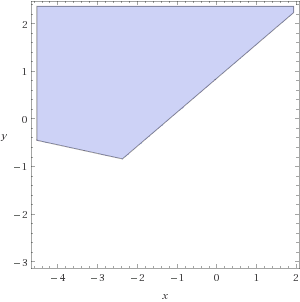
\includegraphics [width=0.3\textwidth ]{img-sol/t2-55a} \par 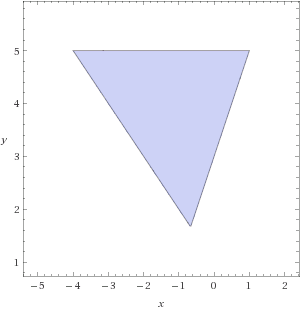
\includegraphics [width=0.3\textwidth ]{img-sol/t2-55b} \par 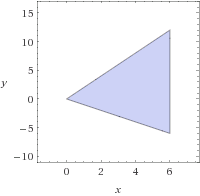
\includegraphics [width=0.3\textwidth ]{img-sol/t2-55c} \par 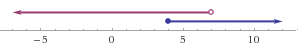
\includegraphics [width=0.4\textwidth ]{img-sol/t2-55d} 
\vspace{0.25cm}
 \item[$\bullet$ ] {\fontfamily{phv}\selectfont\color{blue}\textbf{Autoavaluació:}. }

\vspace{0.25cm}
\item[\fontfamily{phv}\selectfont\color{blue}\textbf{1. }]  \scalebox{0.6}{\simbolclau } 
$-3$
\vspace{0.25cm}
\item[\fontfamily{phv}\selectfont\color{blue}\textbf{2. }]  \scalebox{0.6}{\simbolclau } 
$Q=x^3$; $R=1$
\vspace{0.25cm}
\item[\fontfamily{phv}\selectfont\color{blue}\textbf{3. }]  \scalebox{0.6}{\simbolclau } 
No, si és de grau 4 pot tenir 4 arrels, que poden esser 4 reals, o be 2 arrels reals i 2 complexes o totes 4 complexes.
\vspace{0.25cm}
\item[\fontfamily{phv}\selectfont\color{blue}\textbf{4. }]  \scalebox{0.6}{\simbolclau } 
$x \in [-2, 2]$
\vspace{0.25cm}
\item[\fontfamily{phv}\selectfont\color{blue}\textbf{5. }]  \scalebox{0.6}{\simbolclau } 
$[-1, 15]$
\vspace{0.25cm}
\item[\fontfamily{phv}\selectfont\color{blue}\textbf{6. }]  \scalebox{0.6}{\simbolclau } 
$x \geq 9/5$ 
\vspace{0.25cm}
\item[\fontfamily{phv}\selectfont\color{blue}\textbf{7. }]  \scalebox{0.6}{\simbolclau } 
$x\in (1,2)$
\vspace{0.25cm}


 \needspace{2\baselineskip} 

 \item[\fontfamily{phv}\selectfont\color{blue}\textbf{8}. ]  \scalebox{0.6}{\simbolclau } 
 \begin{tasks}[column-sep=1em, item-indent=1.3333em](4)
	 \task F
	 \task V
	 \task F
	 \task F
\end{tasks}
 \end{enumerate}
\vfill\null
\columnbreak
\def\currentname{Solucions del Tema 3}
\vspace*{0.75cm}

 
 \needspace{5\baselineskip} 
 \scalebox{1.25}{\heading{Solucions del Tema 3}}

\vspace*{0.4cm}
\phantomsection \addcontentsline{toc}{section}{Solucions del Tema 3}
\vspace{0.3cm}

 \needspace{4\baselineskip} 

{\textbf{\em Pàgina 30}} \hrulefill
\begin{enumerate}
\vspace{0.25cm}
\item[\fontfamily{phv}\selectfont\color{blue}\textbf{1. }] 
Si el triangle rectangle té hipotenusa $a$ i catets $b$ i $c$. Es compleix per trigonometria que $b=a\cos \alpha $ i $c=a\sin \alpha $. Si aplicam el teorema de Pitàgores a aquest triangle $a^2 = b^2 + c^2$, trobam que $a^2 = (a\cos \alpha )^2+ (a\sin \alpha )^2$. Finalment, simplificam dividint entre $a^2$ trobam $\sin ^2 \alpha + \cos ^2 \alpha = 1$.
 \end{enumerate}
\vspace{0.3cm}

 \needspace{4\baselineskip} 

{\textbf{\em Pàgina 31}} \hrulefill
\begin{enumerate}
\vspace{0.25cm}
\item[\fontfamily{phv}\selectfont\color{blue}\textbf{2. }] 
$\dfrac {\sin \alpha }{\cos \alpha }=\dfrac {\frac {CO}{H}}{\frac {CC}{H}}=\dfrac {CO}{CC}=\tg \alpha $
 \end{enumerate}
\begin{enumerate}
\vspace{0.25cm}
\item[\fontfamily{phv}\selectfont\color{blue}\textbf{3. }] 
a) Parteix de $\sin ^2 \alpha + \cos ^2 \alpha = 1$ i divideix tot entre $\cos ^2 \alpha $.\par b) Parteix de $\sin ^2 \alpha + \cos ^2 \alpha = 1$ i divideix tot entre $\sin ^2 \alpha $
\vspace{0.25cm}
\item[\fontfamily{phv}\selectfont\color{blue}\textbf{4. }] 
A 45 graus, resulta que CC=CO i per això $\sin 45 = \cos 45$.\par Com que la $\tg 45 = \dfrac {CO}{CC}=1$.
\vspace{0.25cm}
\item[\fontfamily{phv}\selectfont\color{blue}\textbf{5. }] 
$\frac {\pi }{3}$, $\frac {2}{3}\pi $, $\frac {5}{4}\pi $, $\frac {11}{6}\pi $
\vspace{0.25cm}
\item[\fontfamily{phv}\selectfont\color{blue}\textbf{6. }] 
$45^\circ $, $120^\circ $, $270^\circ $, $300^\circ $
\vspace{0.25cm}
\item[\fontfamily{phv}\selectfont\color{blue}\textbf{7. }] 
Els angles d'un triangle sumen $\pi $ radiants. Un angle recte són $\pi /2$ radiants.
\vspace{0.25cm}
\item[\fontfamily{phv}\selectfont\color{blue}\textbf{8. }] 
$\omega =v/R=2$ rad/s. En un minut \linebreak $2$ rad/s $\cdot 60 $s$ = 120 $ rad = 19.1 voltes
 \end{enumerate}
\vspace{0.3cm}

 \needspace{4\baselineskip} 

{\textbf{\em Pàgina 32}} \hrulefill
\begin{enumerate}
\vspace{0.25cm}
\item[\fontfamily{phv}\selectfont\color{blue}\textbf{9. }] 
6 m i 1.5 m
 \end{enumerate}
\begin{enumerate}
\vspace{0.25cm}
\item[\fontfamily{phv}\selectfont\color{blue}\textbf{10. }] 
 $\bullet $ \textbf {120 = 180--60} \par \par $\sin 120=\sin 60$\par $\cos 120=-\cos 60$\par $\tg 120=-\tg 60$\par \par $\bullet $ \textbf {135 = 180--45} \par \par $\sin 135=\sin 45$\par $\cos 135=-\cos 45$\par $\tg 135=-\tg 45$\par \par $\bullet $ \textbf {210 = 180+30} \par \par $\sin 210=-\sin 30$\par $\cos 210=-\cos 30$\par $\tg 210=\tg 30$\par \par $\bullet $ \textbf {315= 360--45} \par \par $\sin 315=-\sin 45$\par $\cos 315=\cos 45$\par $\tg 315=-\tg 45$\par \par $\bullet $ \textbf {390 = 30} \par \par $\sin 390=\sin 30$\par $\cos 390=\cos 30$\par $\tg 390=\tg 30$\par \par $\bullet $ \textbf {3000 = 120} \par \par $\sin 3000=\sin 120$\par $\cos 3000=\cos 120$\par $\tg 3000=\tg 120$\par \par $\bullet $ \textbf {--150 = 210} \par \par $\sin -150=\sin 210$\par $\cos -150=\cos 210$\par $\tg -150=\tg 210$\par \par 
 \end{enumerate}
\vspace{0.3cm}

 \needspace{4\baselineskip} 

{\textbf{\em Pàgina 33}} \hrulefill
\begin{enumerate}
\vspace{0.25cm}
\item[\fontfamily{phv}\selectfont\color{blue}\textbf{11. }] 
Una solució $\arcsin 0,6=36.87^\circ $ l'altre és $180-36.87 =143.13^\circ $
 \end{enumerate}
\begin{enumerate}
\vspace{0.25cm}
\item[\fontfamily{phv}\selectfont\color{blue}\textbf{12. }] 
Una solució $\arctg 4=75.96^\circ $ l'altre és $180+75.96 =255.96^\circ $
\vspace{0.25cm}
\item[\fontfamily{phv}\selectfont\color{blue}\textbf{13. }] 
Una solució $\arccos 0.75=41.41^\circ $ l'altre és $360-41.41 =318.59^\circ $
\vspace{0.25cm}


 \needspace{2\baselineskip} 

 \item[\fontfamily{phv}\selectfont\color{blue}\textbf{14}. ]  \scalebox{0.6}{\simbolclau } 
 \begin{tasks}[column-sep=1em, item-indent=1.3333em](1)
	 \task* $\hat C=33$; $b=26,8$; $c=17,4$
	 \task* $\hat B=67$; $b=66,3$; $c=28,1$
	 \task* $\hat C=39$; $\hat B=51$; $a=396,7$
	 \task* $\hat B=58$; $b=56,01$; $a=66,05$
\end{tasks}
\vspace{0.25cm}
\item[\fontfamily{phv}\selectfont\color{blue}\textbf{15. }]  \scalebox{0.6}{\simbolclau } 
$a=3,46$; $b=1,73$
\vspace{0.25cm}
\item[\fontfamily{phv}\selectfont\color{blue}\textbf{16. }]  \scalebox{0.6}{\simbolclau } 
$\alpha =25,5^\circ $
\vspace{0.25cm}
\item[\fontfamily{phv}\selectfont\color{blue}\textbf{17. }]  \scalebox{0.6}{\simbolclau } 
 $a=25$; $c=20$; $\hat B=36,87^\circ $; $\hat C=53,13^\circ $
 \end{enumerate}
\vspace{0.3cm}

 \needspace{4\baselineskip} 

{\textbf{\em Pàgina 34}} \hrulefill
\begin{enumerate}
\vspace{0.25cm}
\item[\fontfamily{phv}\selectfont\color{blue}\textbf{18. }] 
$\tg \alpha = 5/100$, $\alpha = 2.86^\circ $. $s=\frac {h}{\tg \alpha } = \frac { 100}{\tg 2.86}=2000$ m. Hem caminat 2 km.
 \end{enumerate}
\begin{enumerate}
\vspace{0.25cm}
\item[\fontfamily{phv}\selectfont\color{blue}\textbf{20. }] 
Costats: a = 5.22163 m b = 7.03508 m c = 8 m \par Angles: A = 40 B = 60 C = 80
\vspace{0.25cm}
\item[\fontfamily{phv}\selectfont\color{blue}\textbf{21. }] 
Té dues solucions:\par 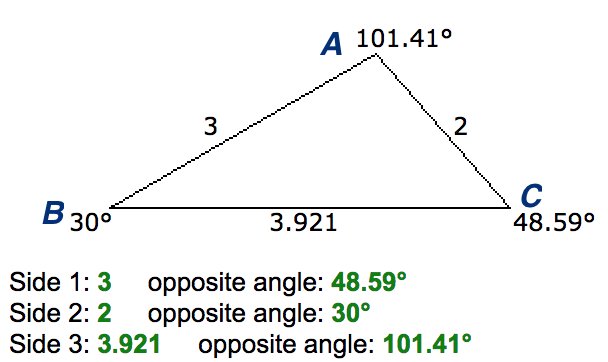
\includegraphics [width=0.4\textwidth ]{img-sol/t3-21a} \par 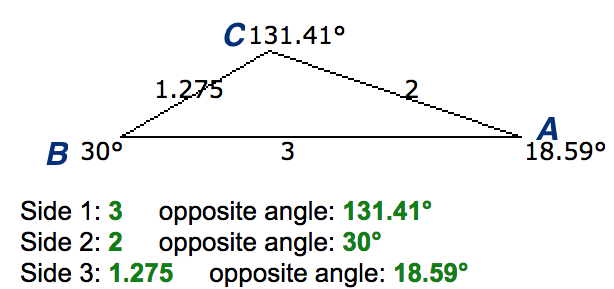
\includegraphics [width=0.4\textwidth ]{img-sol/t3-21b}
\vspace{0.25cm}
\item[\fontfamily{phv}\selectfont\color{blue}\textbf{22. }] 
Solució única:\par 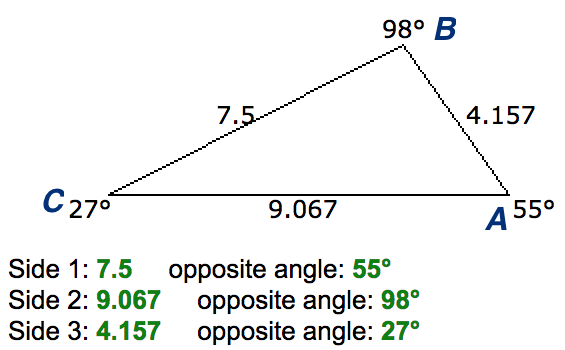
\includegraphics [width=0.4\textwidth ]{img-sol/t3-22}
 \end{enumerate}
\vspace{0.3cm}

 \needspace{4\baselineskip} 

{\textbf{\em Pàgina 35}} \hrulefill
\begin{enumerate}
\vspace{0.25cm}
\item[\fontfamily{phv}\selectfont\color{blue}\textbf{23. }] 
En primer lloc trobam dos costats a partir del radi: $a=4\sqrt {2}\sin 60=2\sqrt {6}$ i $b=4\sqrt {2} \sin 45 = 4$.\par 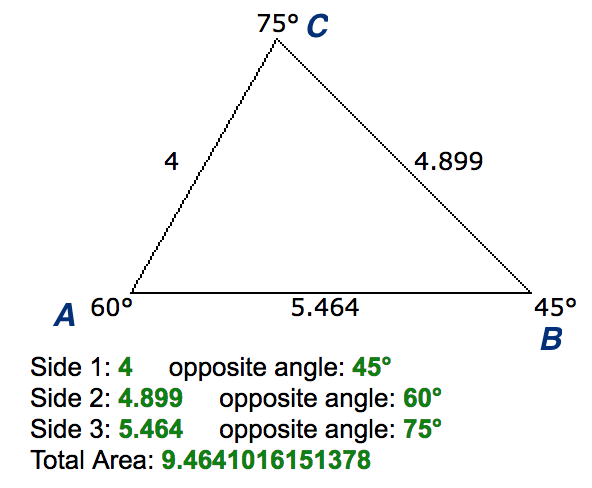
\includegraphics [width=0.4\textwidth ]{img-sol/t3-23}
 \end{enumerate}
\begin{enumerate}
\vspace{0.25cm}
\item[\fontfamily{phv}\selectfont\color{blue}\textbf{24. }] 
En primer lloc resolem el triangle:\par 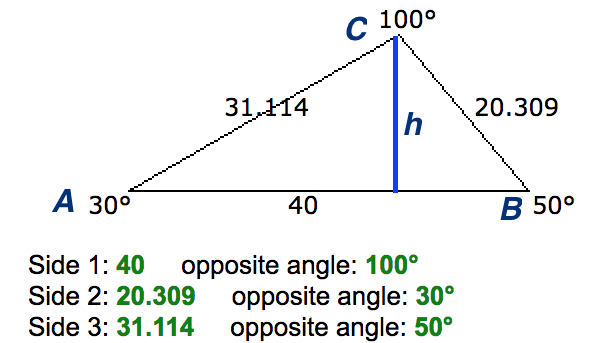
\includegraphics [width=0.4\textwidth ]{img-sol/t3-24}\par Després calculam l'altura del triangle $h=31.1\sin 30=20.31\sin 50=15.6$ m
\vspace{0.25cm}
\item[\fontfamily{phv}\selectfont\color{blue}\textbf{25. }] 
En primer lloc resolem el triangle:\par 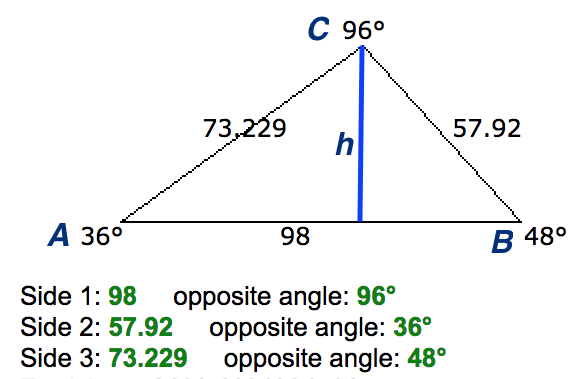
\includegraphics [width=0.4\textwidth ]{img-sol/t3-25}\par Després calculam l'altura del triangle $h=73.23\sin 36=57.92\sin 48=43.04$ m
\vspace{0.25cm}
\item[\fontfamily{phv}\selectfont\color{blue}\textbf{26. }] 
La tangent de l'angle es redueix a la meitat: $\tg \alpha ' = \frac {1}{2}\tg \alpha =\frac {1}{2}\tg 42=0.4502$, el nou angle és $\alpha '=\arctg 0.4502=24.24^\circ $. Evidentment no és la meitat de 42${}^\circ $.
\vspace{0.25cm}
\item[\fontfamily{phv}\selectfont\color{blue}\textbf{27. }] 
En primer lloc resolem el triangle:\par 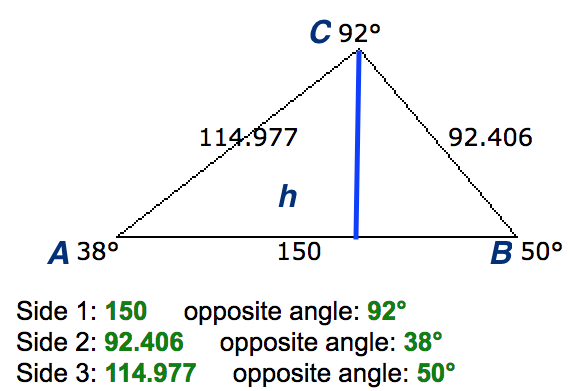
\includegraphics [width=0.4\textwidth ]{img-sol/t3-27}\par Les distàncies de cadascú a l'estel són 115 m i 92.4 m. Després l'altura del triangle $h=114.98\sin 38=92.406\sin 50=70.79$ m
\vspace{0.25cm}
\item[\fontfamily{phv}\selectfont\color{blue}\textbf{28. }] 
L'angle del triangle és $180-42=138$. En primer lloc resolem el triangle:\par 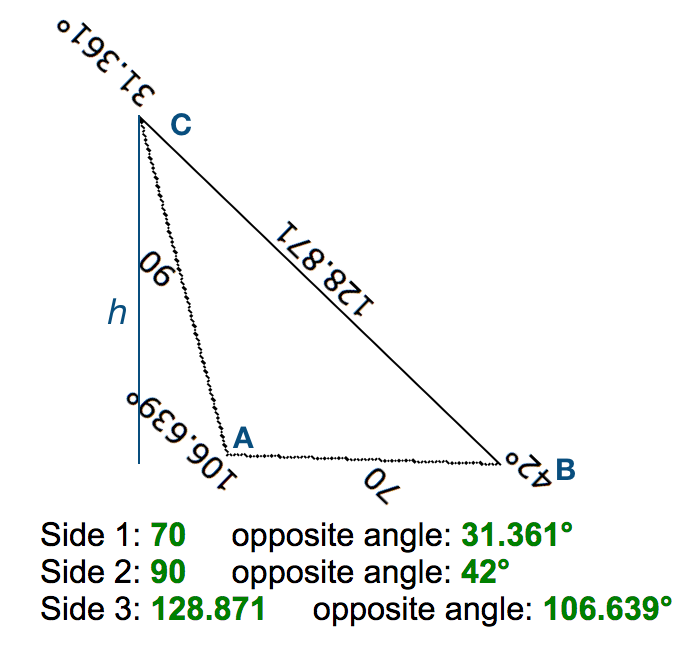
\includegraphics [width=0.4\textwidth ]{img-sol/t3-28}\par L'altre cable mesura 128.87 m. La distància del globus al terra $h=128.87\sin 42=86.23$ m
 \end{enumerate}
\vspace{0.3cm}

 \needspace{4\baselineskip} 

{\textbf{\em Pàgina 36}} \hrulefill
\begin{enumerate}
\vspace{0.25cm}
\item[\fontfamily{phv}\selectfont\color{blue}\textbf{29. }] 
$\hat A=28.52^\circ $, $\hat B=32.82^\circ $, $\hat C=118.66^\circ $
 \end{enumerate}
\begin{enumerate}
\vspace{0.25cm}
\item[\fontfamily{phv}\selectfont\color{blue}\textbf{30. }] 
Triangle:\par 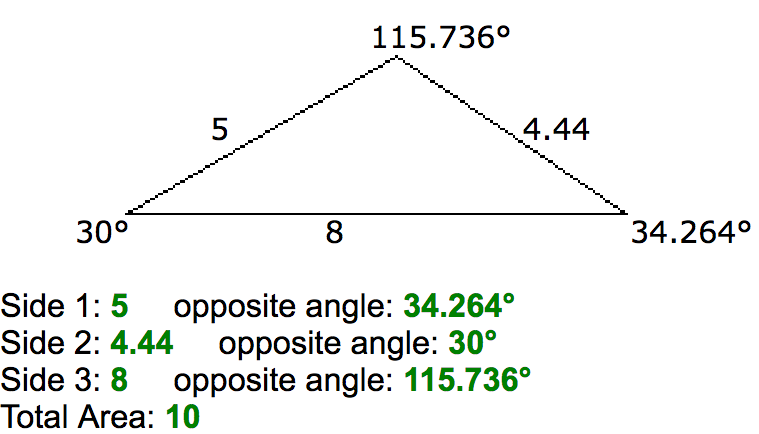
\includegraphics [width=0.4\textwidth ]{img-sol/t3-30}
\vspace{0.25cm}
\item[\fontfamily{phv}\selectfont\color{blue}\textbf{31. }] 
$\hat A=21.79^\circ $, $\hat B=38.21^\circ $, $\hat C=120^\circ $
\vspace{0.25cm}
\item[\fontfamily{phv}\selectfont\color{blue}\textbf{32. }] 
Solució 1:\par 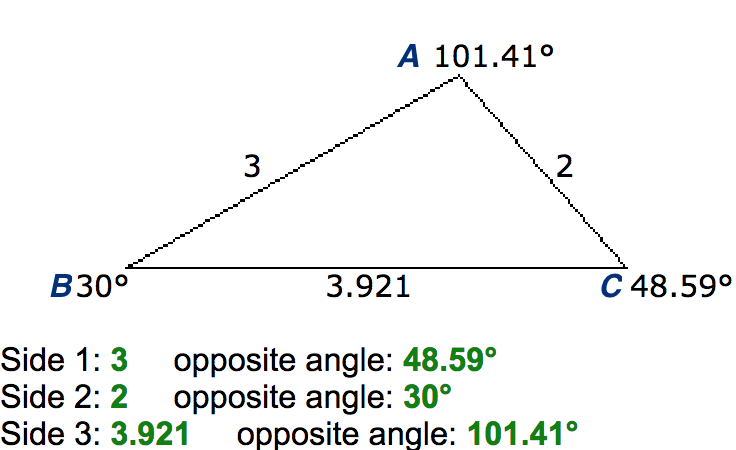
\includegraphics [width=0.4\textwidth ]{img-sol/t3-32a} \par Solució 2:\par 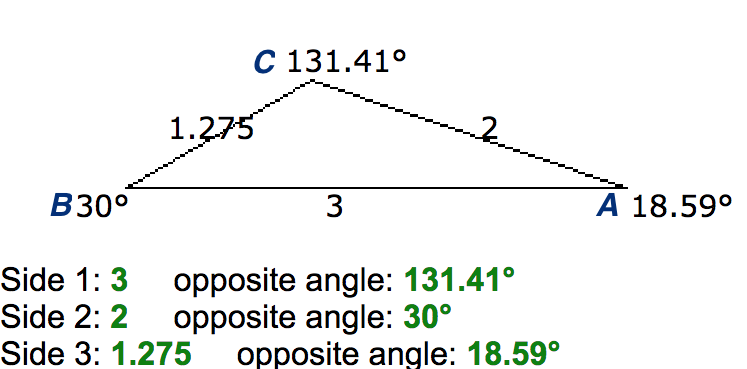
\includegraphics [width=0.4\textwidth ]{img-sol/t3-32b} 
\vspace{0.25cm}
\item[\fontfamily{phv}\selectfont\color{blue}\textbf{33. }] 
El radi de la circumferència $R=L/2\pi =5.57$ cm. El costat de l'heptàgon és $c=4.83$ cm i l'apotema $a_p=5.02$ i l'àrea $A=84.9$ cm$^2$.\par 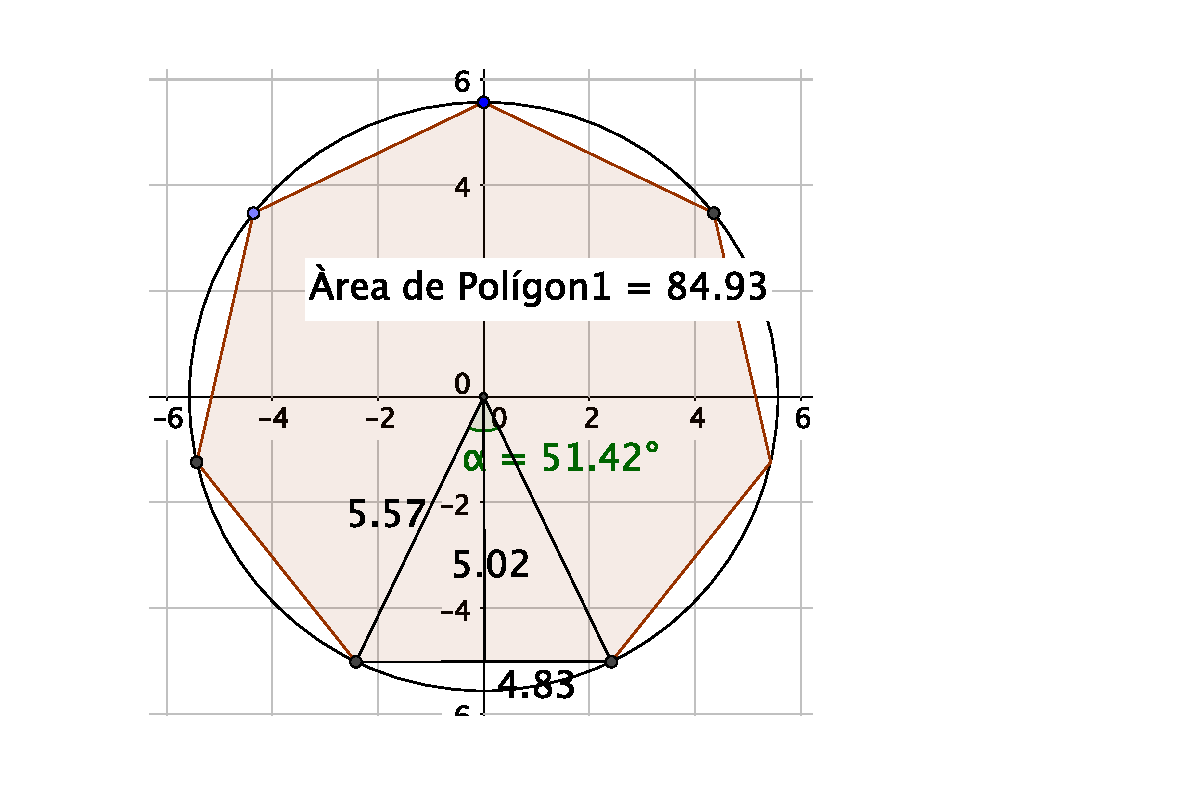
\includegraphics [width=0.3\textwidth ]{img-sol/t3-33}
\vspace{0.25cm}
\item[\fontfamily{phv}\selectfont\color{blue}\textbf{34. }] 
Les distàncies en km recorregudes per cada vaixell són: $15\cdot 5 \, h \cdot 1.85=157.25$ km i $26\cdot 3.5 \,h \cdot 1.85=168.35$ km. A les 15:00 es troben separats per 291.43 km que és superior a l'abast de le radi.\par 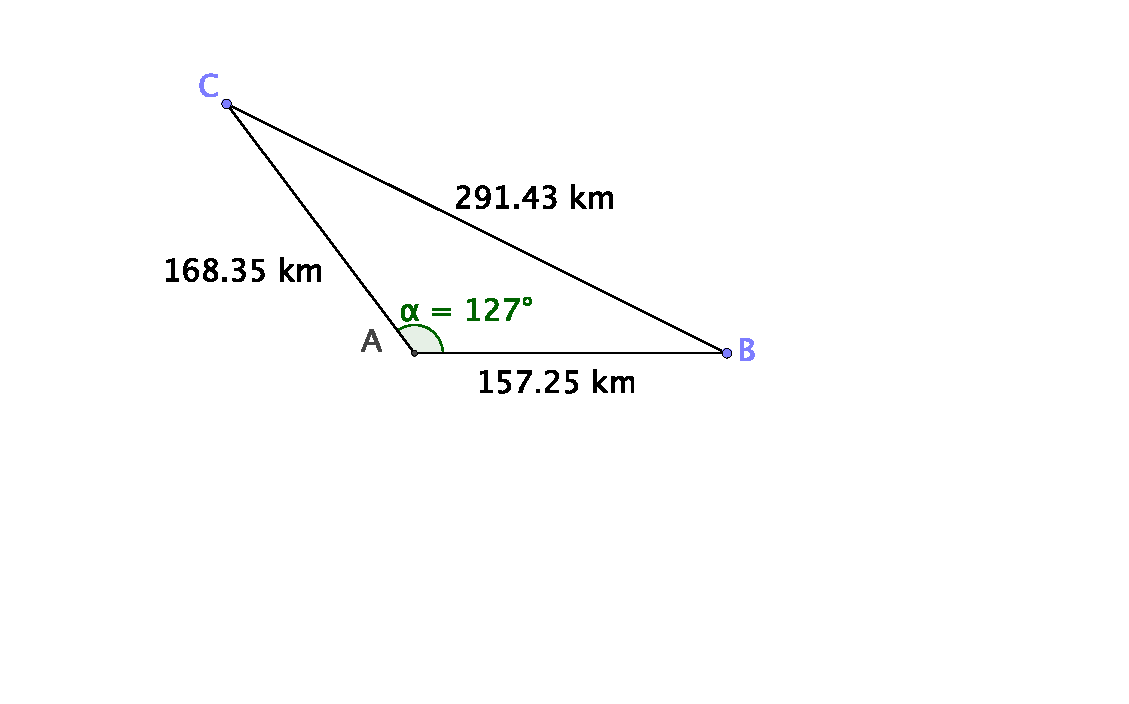
\includegraphics [width=0.4\textwidth ]{img-sol/t3-34}
\vspace{0.25cm}


 \needspace{2\baselineskip} 

 \item[\fontfamily{phv}\selectfont\color{blue}\textbf{35}. ] 
 \begin{tasks}[column-sep=1em, item-indent=1.3333em](1)
	 \task*  $A=24.52$; $C=125.38$; $c=9.78$
	 \task $B=75$; $a=14.64$; $c=17.93$
	 \task No existeix cap triangle
	 \task $A=77.36$; $B=C=51.32$
	 \task* Solució 1: $B=62.1$; $C=72.9$; $c=54.1$. Solució 2: $B=17.1$; $C=117.9$; $c=50$.
\end{tasks}
\vspace{0.25cm}
\item[\fontfamily{phv}\selectfont\color{blue}\textbf{36. }] 
El costat del polígon és $c=3.53$ cm i l'apotema $a_p=2,43$ i l'àrea $A=21.4$ cm$^2$.\par 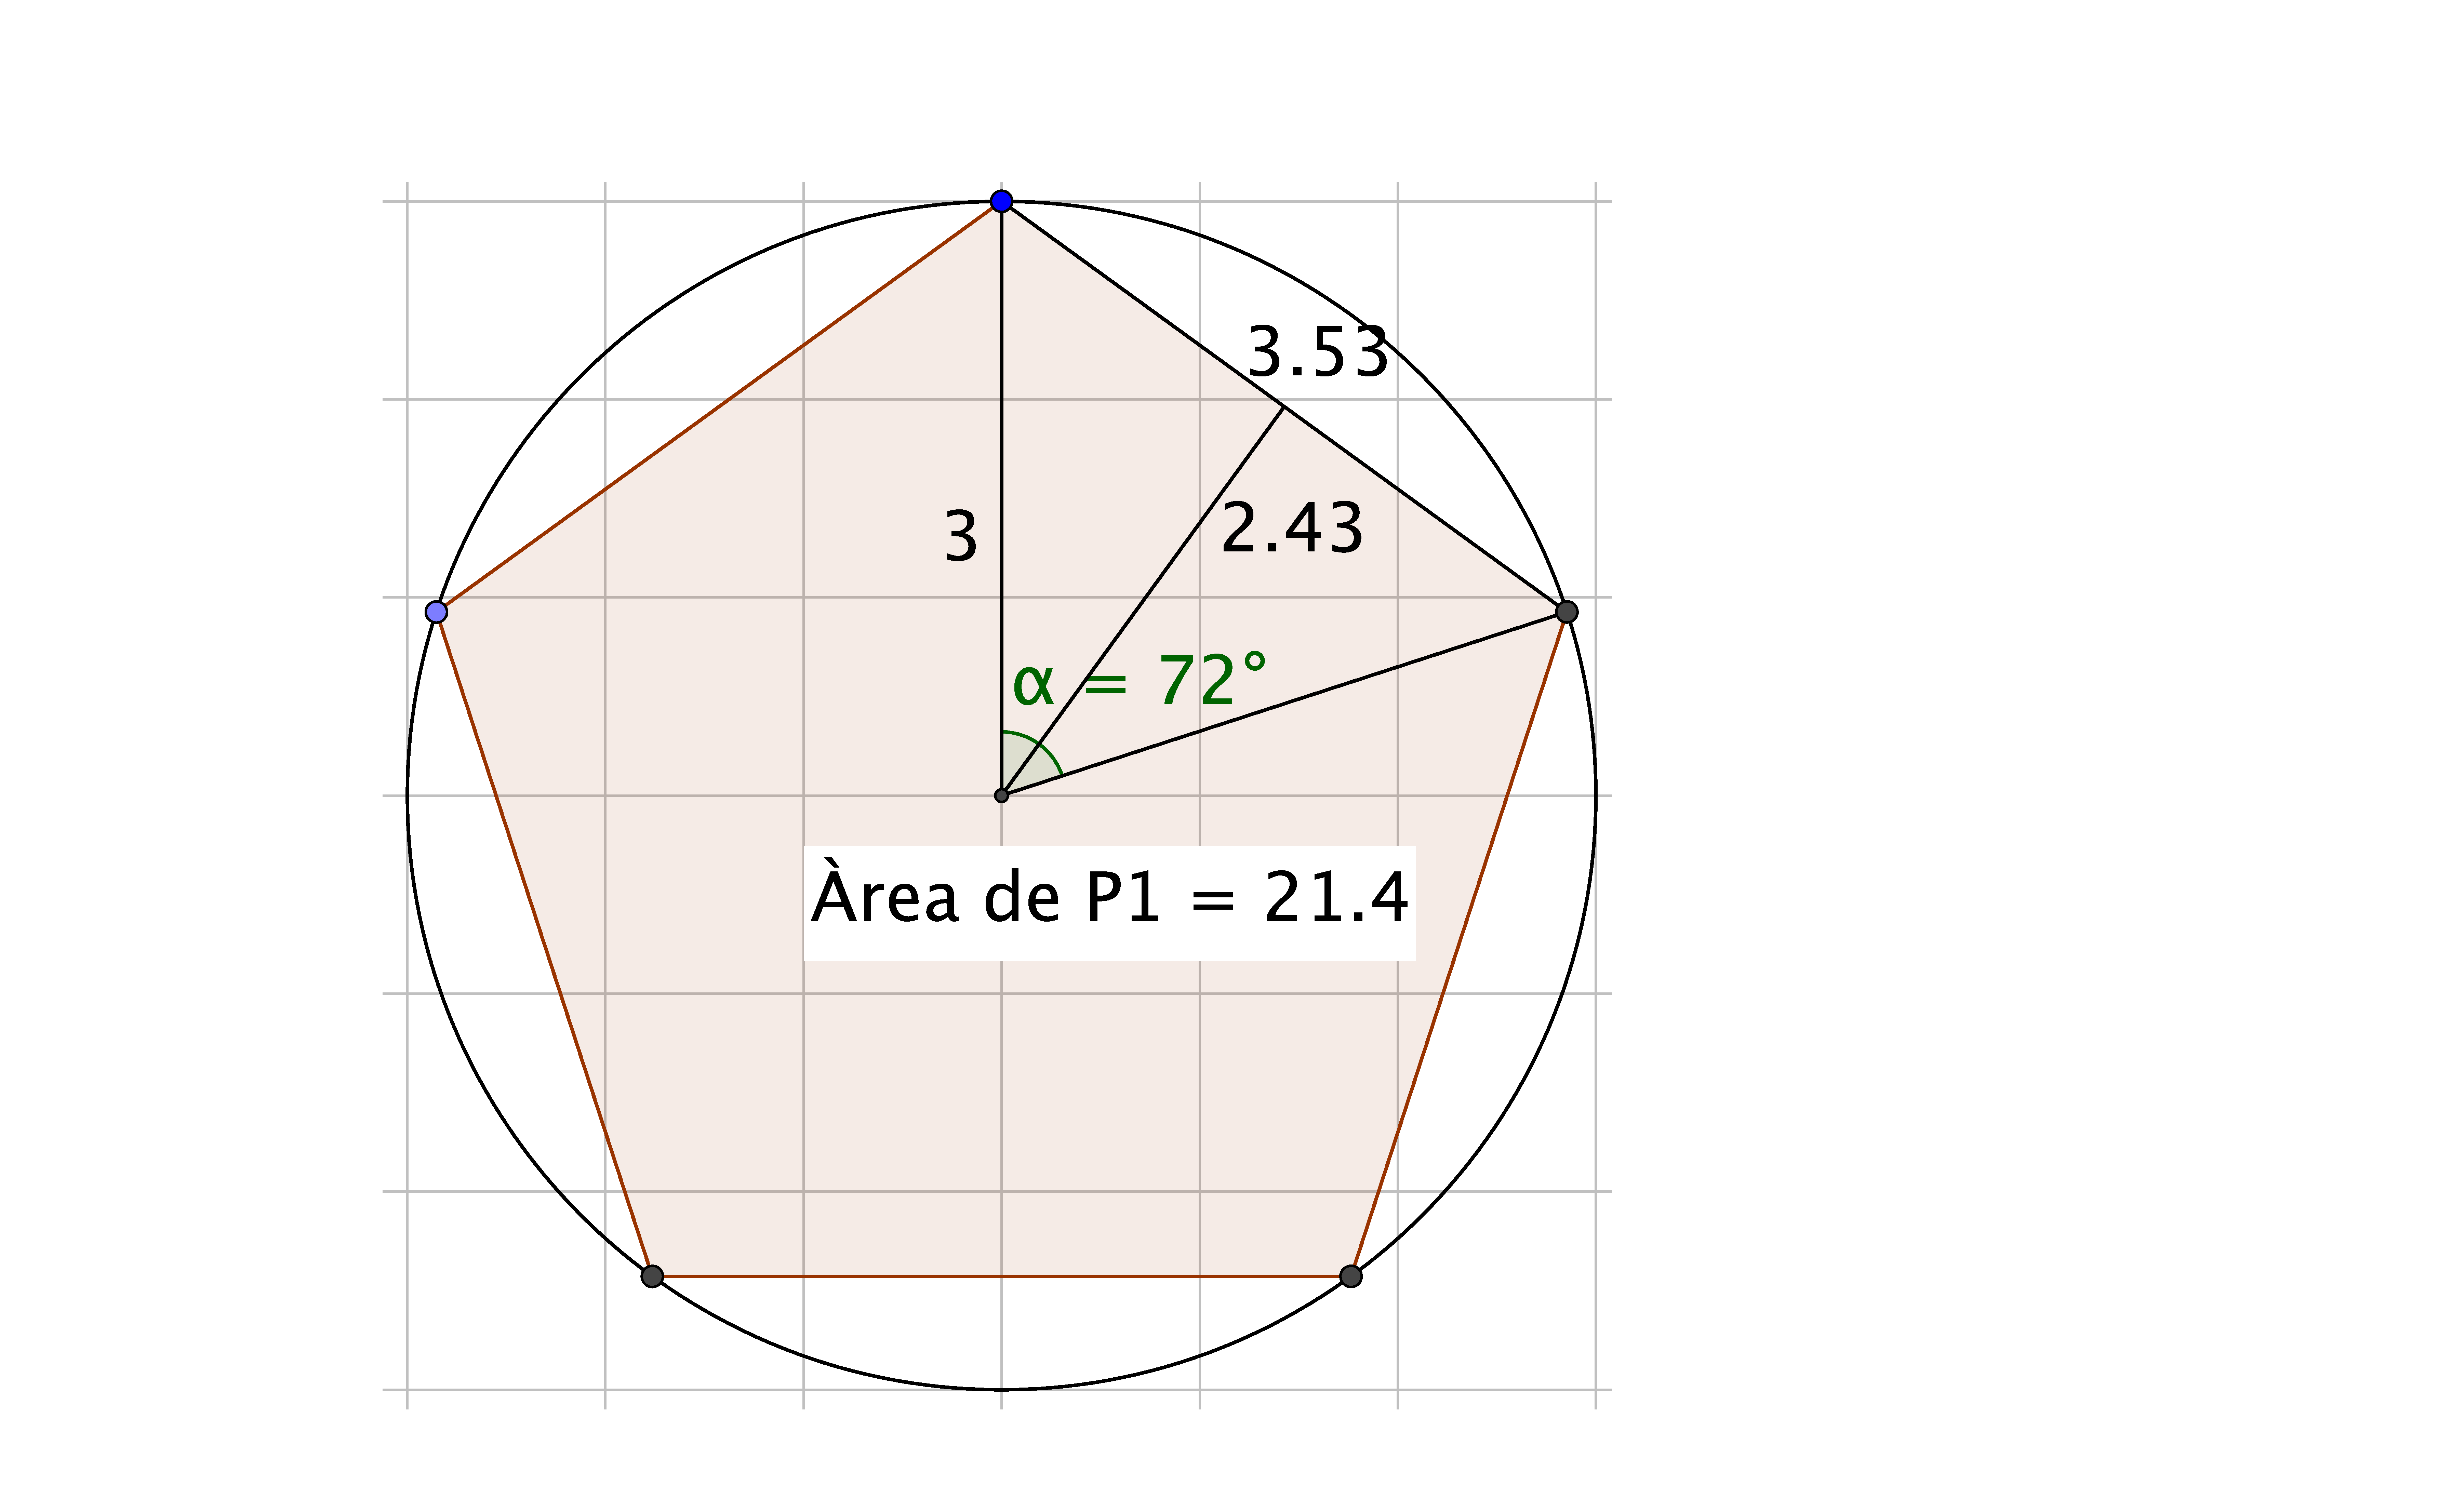
\includegraphics [width=0.3\textwidth ]{img-sol/t3-36}
 \end{enumerate}
\vspace{0.3cm}

 \needspace{4\baselineskip} 

{\textbf{\em Pàgina 37}} \hrulefill
\begin{enumerate}
\vspace{0.25cm}
\item[\fontfamily{phv}\selectfont\color{blue}\textbf{37. }] 
Construïm el triangle rectangle de la figura. Té de catets $c=5-3=2$ i $b=\dfrac {3}{\tg 21} - \dfrac {5}{\tg 43}=2.453$. La distància és la hipotenusa del triangle $a=\sqrt {b^2+c^2}=3.165$ km  \par 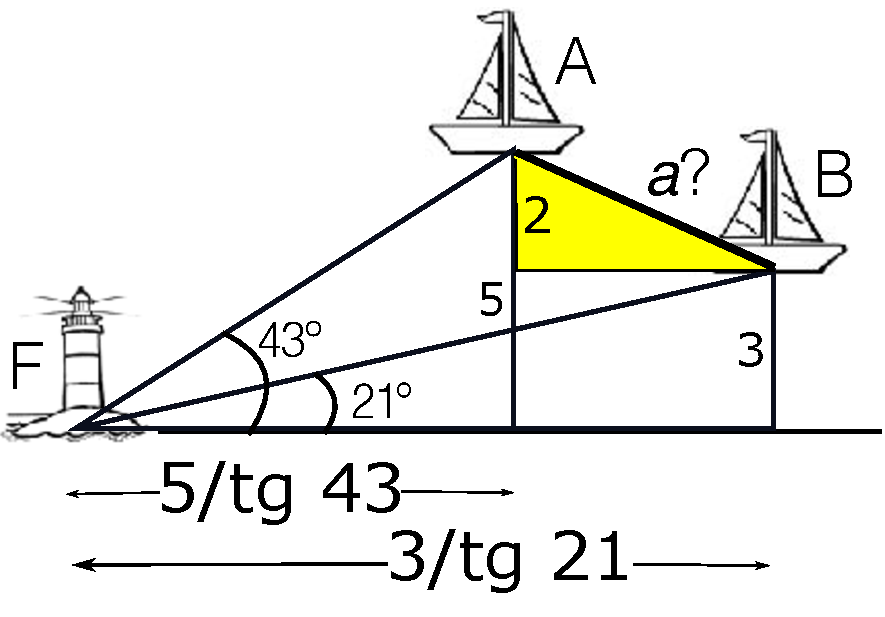
\includegraphics [width=0.4\textwidth ]{img-sol/t3-37} 
 \end{enumerate}
\begin{enumerate}
\vspace{0.25cm}
\item[\fontfamily{phv}\selectfont\color{blue}\textbf{38. }] 
Perímetre: 457.16 m. Àrea: 8030,1 m$^2$.  \par 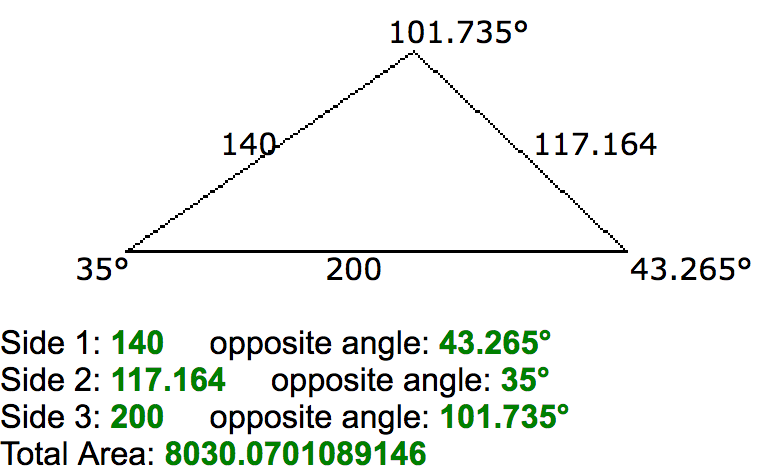
\includegraphics [width=0.42\textwidth ]{img-sol/t3-38} 
\vspace{0.25cm}
\item[\fontfamily{phv}\selectfont\color{blue}\textbf{39. }] 
Del triangle rectangle d'abaix trobam la base com $b=250\cos 30=216.51$ m. Del triangle rectangle complet $\tg 40 = \dfrac {H}{216.51}$, aïllam $H=181.67$ m.
\vspace{0.25cm}


 \needspace{2\baselineskip} 

 \item[\fontfamily{phv}\selectfont\color{blue}\textbf{40}. ] 
 \begin{tasks}[column-sep=1em, item-indent=1.3333em](3)
	 \task 100 m
	 \task 86.60 m
	 \task 90$^\circ $
\end{tasks}
\vspace{0.25cm}
\item[\fontfamily{phv}\selectfont\color{blue}\textbf{41. }] 
Primer trobam els angles que falten. Es un triangle d'angles 80, 60, 40. Aplicam el teorema del sinus: $\dfrac {h}{\sin 80}=\dfrac {15}{\sin 40}$. Aïllam $h =22.98$ m.
\vspace{0.25cm}
\item[\fontfamily{phv}\selectfont\color{blue}\textbf{42. }] 
$d(B, E) = 67.59$; $h = 56,7135$ m
\vspace{0.25cm}
\item[\fontfamily{phv}\selectfont\color{blue}\textbf{43. }] 
Des de $B$ les altres dues ciutats es veuen amb un angle de 49.11$^\circ $. \par 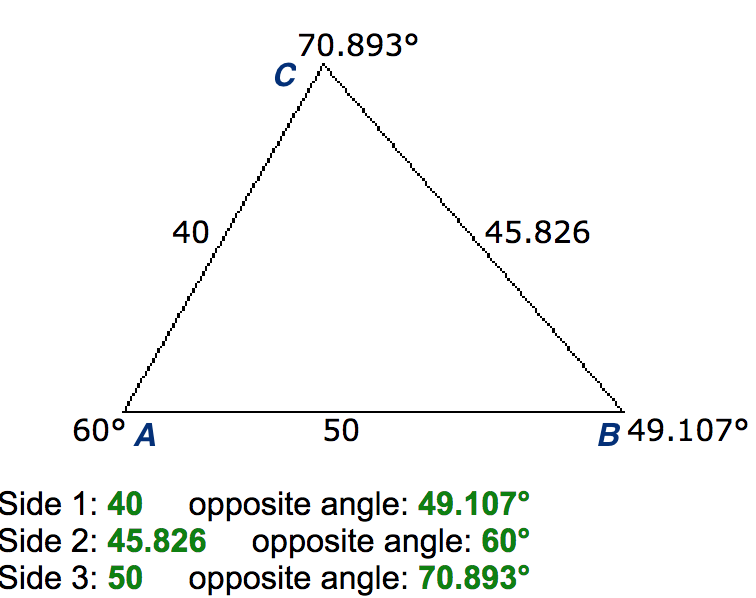
\includegraphics [width=0.43\textwidth ]{img-sol/t3-43}
\vspace{0.25cm}
\item[\fontfamily{phv}\selectfont\color{blue}\textbf{44. }]  \scalebox{0.6}{\simbolclau } 
$d=35,49$ km
 \end{enumerate}
\vspace{0.3cm}

 \needspace{4\baselineskip} 

{\textbf{\em Pàgina 38}} \hrulefill
\begin{enumerate}
\vspace{0.25cm}
\item[\fontfamily{phv}\selectfont\color{blue}\textbf{45. }]  \scalebox{0.6}{\simbolcompass } 
Del triangle $\widehat {CAD}$ troba $\overline {AD}=74.16$ km, del triangle $\widehat {CBD}$ troba $\overline {BD}=52.05$ km pel teorema del sinus i finalment del triangle $\widehat {ADB}$ troba $\overline {AB}=24$ km pel teorema del cosinus.
 \end{enumerate}
\begin{enumerate}
\vspace{0.25cm}
\item[\fontfamily{phv}\selectfont\color{blue}\textbf{46. }]  \scalebox{0.6}{\simbolclau } 
cim A=827 m, cim B=751 m, distància entre cims AB=1687.3 m
\vspace{0.25cm}
\item[\fontfamily{phv}\selectfont\color{blue}\textbf{47. }] 
Es trobava a 17.32 m de l'Abadia de Westminster i a 32.68 m del Big Ben. L'altura del Big Ben és 32.68 m ja que es veu amb un angle de 45$^\circ $. \par 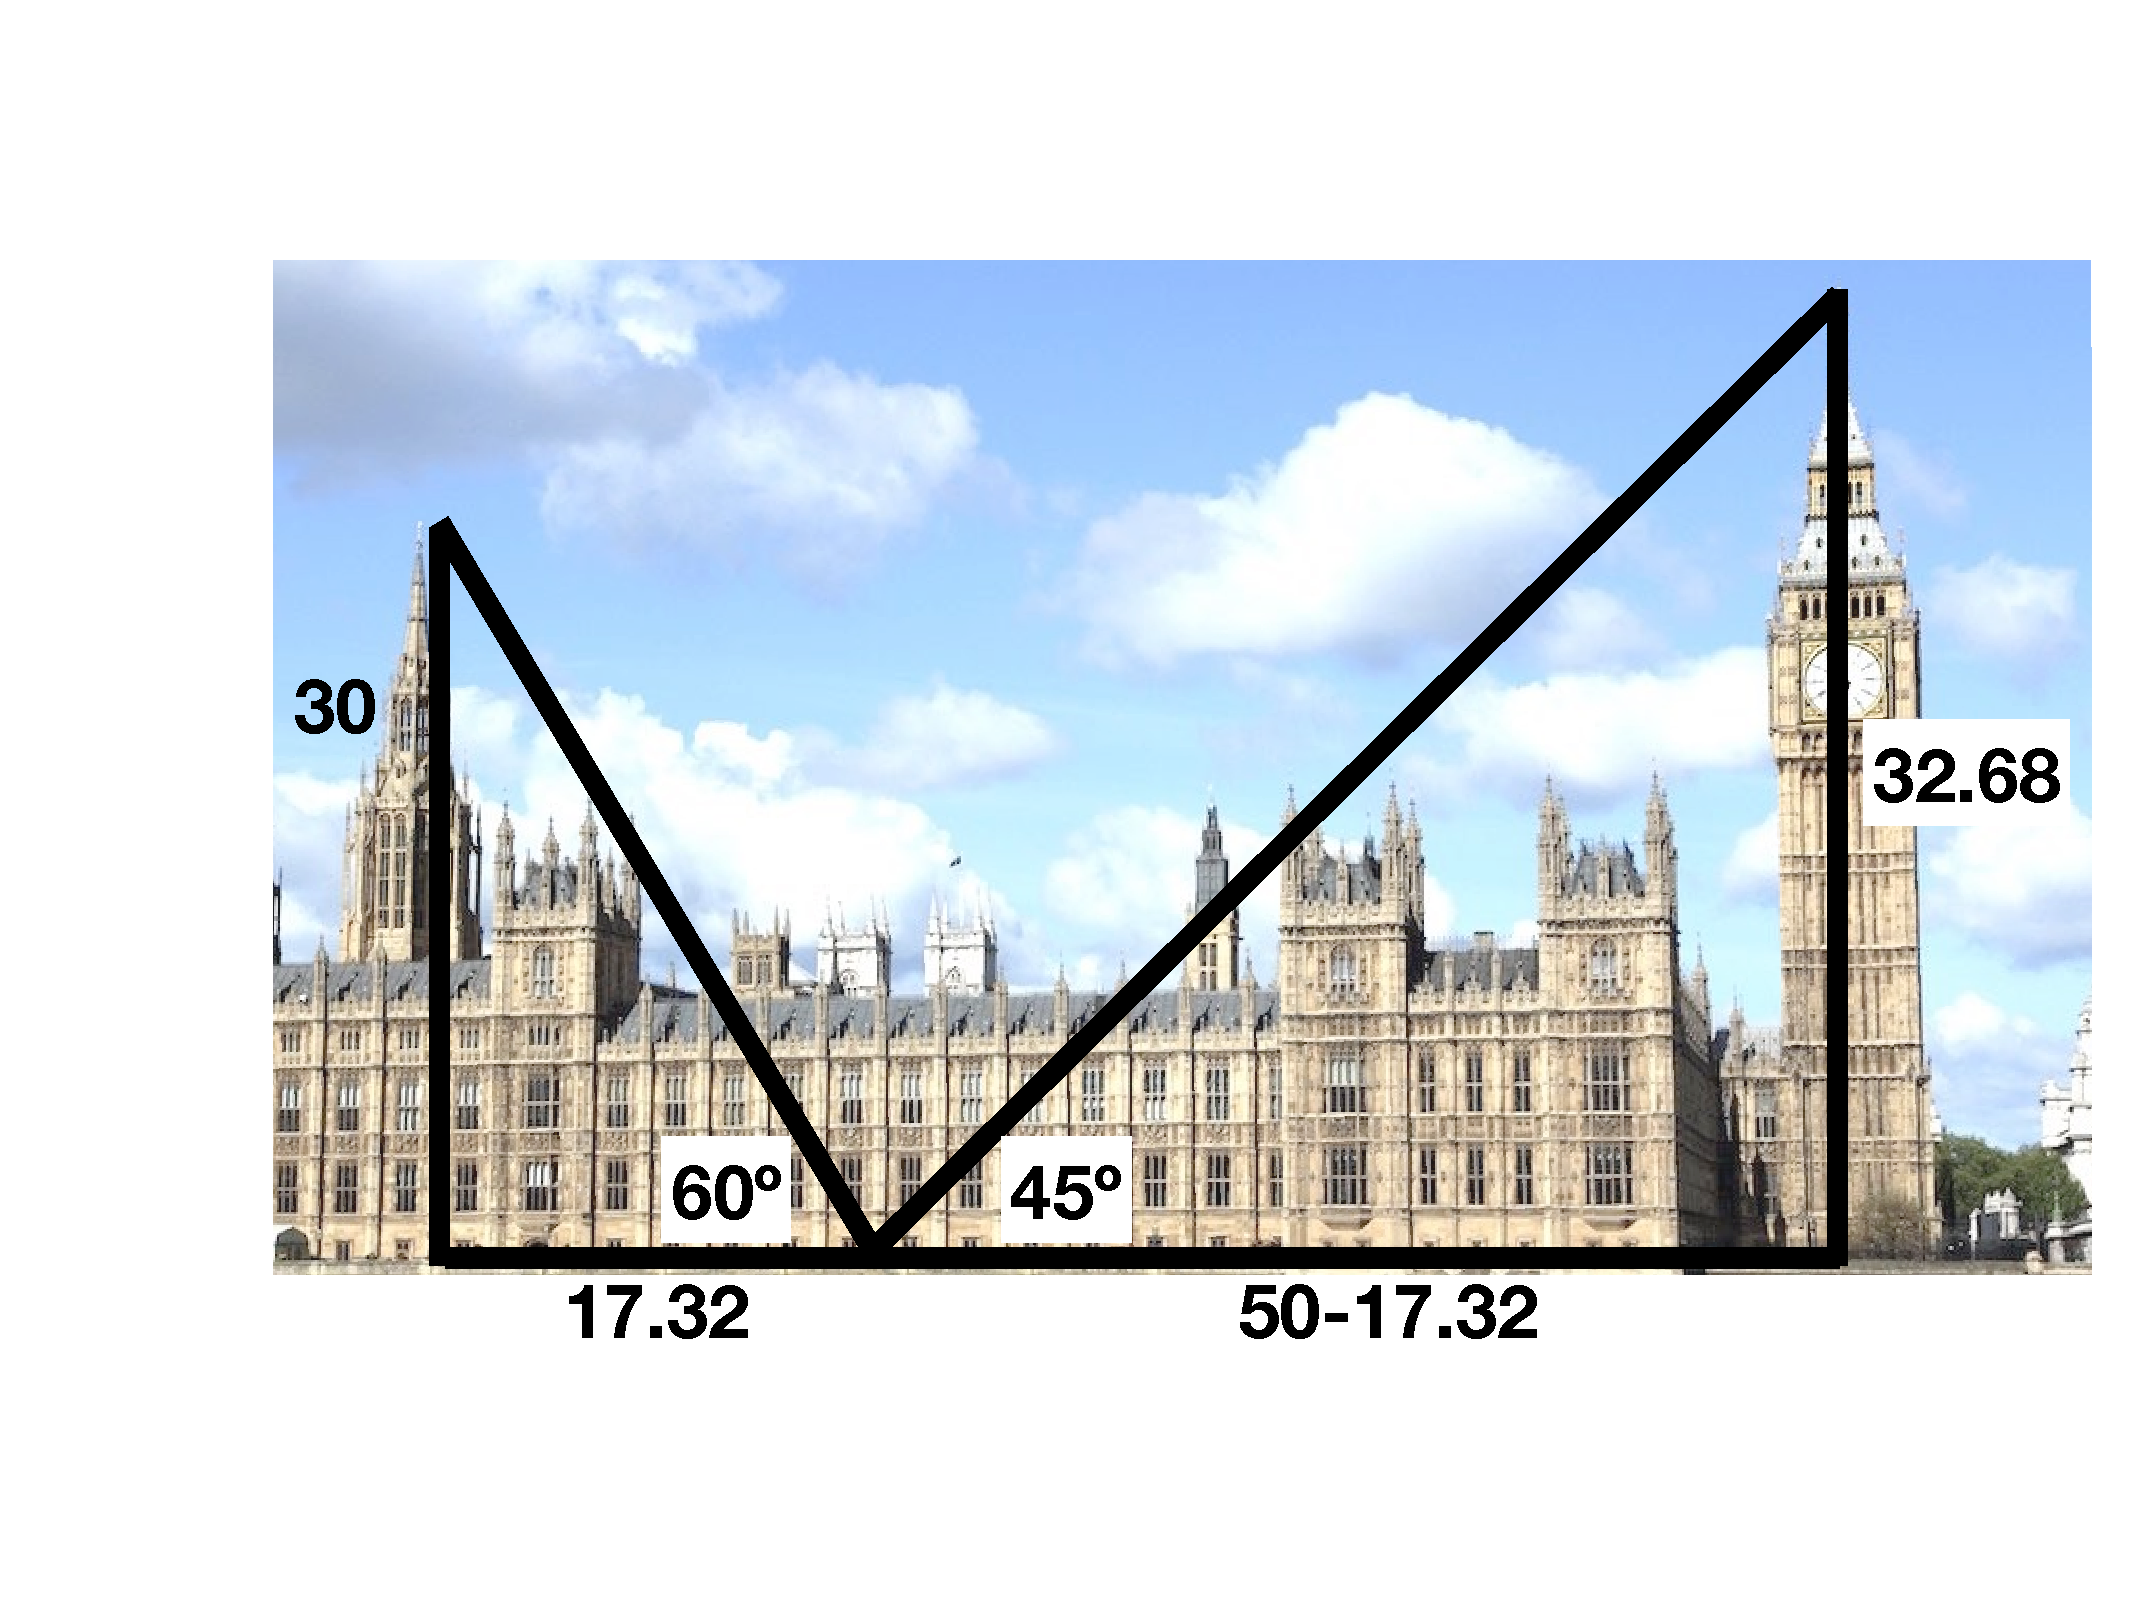
\includegraphics [width=0.4\textwidth ]{img-sol/t3-47}
 \end{enumerate}
\vspace{0.3cm}

 \needspace{4\baselineskip} 

{\textbf{\em Pàgina 39}} \hrulefill
\begin{enumerate}
\vspace{0.25cm}
\item[\fontfamily{phv}\selectfont\color{blue}\textbf{49. }] 
15=45-30; $\sin 15=\sin 45\cos 30 - \cos 45 \sin 30= \dfrac {\sqrt {6}-\sqrt {2}}{4}$ \par $\cos 15=\cos 45\cos 30 + \sin 43 \sin 30= \dfrac {\sqrt {6}+\sqrt {2}}{4}$ \par $\tg 15=2-\sqrt {3}$ 
 \end{enumerate}
\begin{enumerate}
\vspace{0.25cm}
\item[\fontfamily{phv}\selectfont\color{blue}\textbf{50. }] 
30=90-60; $\sin 30=\sin 90\cos 60 - \cos 90 \sin 60= \cos 60 = \dfrac {1}{2}$ \par $\cos 30=\cos 90\cos 60 + \sin 90 \sin 60= \sin 60 =\dfrac {\sqrt {3}}{2}$ \par $\tg 60=\sqrt {3}$ 
\vspace{0.25cm}
\item[\fontfamily{phv}\selectfont\color{blue}\textbf{51. }] 
$\sin (90-\alpha )=\sin 90 \cos \alpha - \cos 90 \sin \alpha = \cos \alpha $,\par $\cos (90-\alpha )=\cos 90 \cos \alpha + \sin 90 \sin \alpha =\sin \alpha $ i $\tg (90-\alpha )= 1/\tg \alpha $
\vspace{0.25cm}
\item[\fontfamily{phv}\selectfont\color{blue}\textbf{52. }] 
$22.5 = 45/2$, $\sin 22.5= \dfrac {\sqrt {2-\sqrt {2}}}{2}$, $\cos 22.5= \dfrac {\sqrt {2+\sqrt {2}}}{2}$, $\tg 22.5= \sqrt {3-2\sqrt {2}}$\par $11.25 = 22.5/2$, $\sin 11.25= \frac {\sqrt {2-\sqrt {2+\sqrt {2}}}}{2}$, $\cos 11.25= \frac {\sqrt {2+\sqrt {2+\sqrt {2}}}}{2}$, $\tg 11.25= -1-\sqrt {2}+\sqrt {2(2+\sqrt {2})}$ 
\vspace{0.25cm}
\item[\fontfamily{phv}\selectfont\color{blue}\textbf{53. }] 
$45 = 90/2$, $\sin 45= \sqrt {\frac {1-\cos 90}{2}}=\frac {\sqrt {2}}{2}$, $\cos 45= \sqrt {\frac {1+\cos 90}{2}}=\dfrac {\sqrt {2}}{2}$,\par $\tg 45= \sqrt {\dfrac {1-\cos 90}{1+\cos 90}}=1$
\vspace{0.25cm}
\item[\fontfamily{phv}\selectfont\color{blue}\textbf{54. }]  \scalebox{0.6}{\simbolcompass } 
Treu factor comú $\cos \alpha $ i utilitza la relació fonamental.
\vspace{0.25cm}
\item[\fontfamily{phv}\selectfont\color{blue}\textbf{55. }]  \scalebox{0.6}{\simbolcompass } 
Desenvolupa el quadrat amb la identitat notable $(a+b)^2 = a^2 + b^2 + 2ab$. Empra la relació fonamental i la fórmula de $\sin 2\alf $.
\vspace{0.25cm}
\item[\fontfamily{phv}\selectfont\color{blue}\textbf{56. }]  \scalebox{0.6}{\simbolcompass } 
Utilitza les relacions de l'angle oposat $\cos (-x)=\cos x$, $\sin (-x)=-\sin x$, $\tg (-x)=-\tg x$.
\vspace{0.25cm}
\item[\fontfamily{phv}\selectfont\color{blue}\textbf{57. }]  \scalebox{0.6}{\simbolcompass } 
Expressa $\tg \alf $ i $\cotg \alf $ com a quocients de sinus i cosinus. Després realitza la suma de fraccions amb el mínim comú múltiple. Finalment utilitza la relació fonamental.
\vspace{0.25cm}
\item[\fontfamily{phv}\selectfont\color{blue}\textbf{58. }]  \scalebox{0.6}{\simbolcompass } 
Escriu $\sin (3\alf ) = \sin (\alf +2\alf )$. Aplica la fórmula de la suma d'angles i tot seguit les fórmules de l'angle doble. Finalment opera, simplifica i treu factor comú $\sin \alf $.
\vspace{0.25cm}
\item[\fontfamily{phv}\selectfont\color{blue}\textbf{59. }]  \scalebox{0.6}{\simbolcompass } 
Escriu $\cos (4\alf ) = \cos (2\alf +2\alf )$. Aplica la fórmula de la suma d'angles i tot seguit les fórmules de l'angle doble. Finalment opera i simplifica.
 \end{enumerate}
\vspace{0.3cm}

 \needspace{4\baselineskip} 

{\textbf{\em Pàgina 40}} \hrulefill
\begin{enumerate}
\vspace{0.25cm}


 \needspace{2\baselineskip} 

 \item[\fontfamily{phv}\selectfont\color{blue}\textbf{60}. ] 
 \begin{tasks}[column-sep=1em, item-indent=1.3333em](2)
	 \task 2
	 \task 1
	 \task 1
	 \task $\cotg x$
\end{tasks}
 \end{enumerate}
\begin{enumerate}
\vspace{0.25cm}


 \needspace{2\baselineskip} 

 \item[\fontfamily{phv}\selectfont\color{blue}\textbf{63}. ] 
 \begin{tasks}[column-sep=1em, item-indent=1.3333em](2)
	 \task $\sqrt {2}\sin a$
	 \task $-\sqrt {3}\sin a$
\end{tasks}
\vspace{0.25cm}


 \needspace{2\baselineskip} 

 \item[\fontfamily{phv}\selectfont\color{blue}\textbf{65}. ] 
 \begin{tasks}[column-sep=1em, item-indent=1.3333em](1)
	 \task* $x=120+n\cdot 360$ i $x=240+n\cdot 360$
	 \task $x=60+n 180$
	 \task* $x=225+n\cdot 360$ i $x=315+n\cdot 360$
\end{tasks}
\vspace{0.25cm}


 \needspace{2\baselineskip} 

 \item[\fontfamily{phv}\selectfont\color{blue}\textbf{66}. ] 
 \begin{tasks}[column-sep=1em, item-indent=1.3333em](1)
	 \task $x=30+n\cdot 60$
	 \task $x=67.5+n\cdot 90$
	 \task $x=67.5+n\cdot 90$
\end{tasks}
 \end{enumerate}
\vspace{0.3cm}

 \needspace{4\baselineskip} 

{\textbf{\em Pàgina 41}} \hrulefill
\begin{enumerate}
\vspace{0.25cm}


 \needspace{2\baselineskip} 

 \item[\fontfamily{phv}\selectfont\color{blue}\textbf{67}. ] 
 \begin{tasks}[column-sep=1em, item-indent=1.3333em](1)
	 \task $x=n\cdot 60$ i $x=n\cdot 90$
	 \task* $x=30+n\cdot 60$ i $x=n\cdot 180$
\end{tasks}
 \end{enumerate}
\begin{enumerate}
\vspace{0.25cm}


 \needspace{2\baselineskip} 

 \item[\fontfamily{phv}\selectfont\color{blue}\textbf{68}. ] 
 \begin{tasks}[column-sep=1em, item-indent=1.3333em](1)
	 \task* $x=90+n\cdot 360$ i $x=n\cdot 360$
	 \task $x=90+n\cdot 180$
	 \task* $x=60+n\cdot 180$ i $x=120+n\cdot 180$
	 \task* $x=90+n\cdot 180$ i $x=68.53+n\cdot 360$ i $x=291.47+n\cdot 360$
\end{tasks}
\vspace{0.25cm}


 \needspace{2\baselineskip} 

 \item[\fontfamily{phv}\selectfont\color{blue}\textbf{69}. ] 
 \begin{tasks}[column-sep=1em, item-indent=1.3333em](1)
	 \task* $x=90+n\cdot 180$ i $x=60+n\cdot 180$ i $x=120+n\cdot 180$
	 \task* $x=n \cdot 180$ i $x=45+n\cdot 90$
\end{tasks}
\vspace{0.25cm}


 \needspace{2\baselineskip} 

 \item[\fontfamily{phv}\selectfont\color{blue}\textbf{70}. ] 
 \begin{tasks}[column-sep=1em, item-indent=1.3333em](1)
	 \task* Anomenam $c=\cos x$. Només si $c=0$; dóna $x=90+n\cdot 180$
	 \task* Només si $c=\pm 1/\sqrt {3}$; dóna $x=54.73+n\cdot 180$ i $x=125.27+n\cdot 180$
	 \task* Només prové solució de $c=0.5639$; dóna $x=55.67+n\cdot 360$ i $x=304.33+n\cdot 360$
\end{tasks}
\vspace{0.25cm}


 \needspace{2\baselineskip} 

 \item[\fontfamily{phv}\selectfont\color{blue}\textbf{71}. ] 
 \begin{tasks}[column-sep=1em, item-indent=1.3333em](1)
	 \task* $x=n\cdot 180$ i $x=90+n\cdot 360$
	 \task* $x=90+n\cdot 180$ i $x=n\cdot 360$
	 \task* $x=35.26+n\cdot 180$ i $x=144.74+n\cdot 180$
	 \task* $x=15+n\cdot 180$ i $x=75+n\cdot 180$
\end{tasks}
\vspace{0.25cm}


 \needspace{2\baselineskip} 

 \item[\fontfamily{phv}\selectfont\color{blue}\textbf{72}. ] 
 \begin{tasks}[column-sep=1em, item-indent=1.3333em](1)
	 \task* Sumar les dues equacions i aplica identitat fonamental $x=1;\,y=90+n\cdot 180$
	 \task* Suma les dues i aplica sinus d'una suma. Fes el mateix restant-les\par Arribes al sistema $\left \{\begin {array}{l} \sin (x+y)=1 \\ \sin (x-y)=1/2 \end {array} \right .$.\par Trobam $x=60+n\cdot 180;\,y=30+n'\cdot 180$ i $x=120+n\cdot 180;\,y=150+n'\cdot 180$ 
\end{tasks}
\vspace{0.25cm}


 \needspace{2\baselineskip} 

 \item[\fontfamily{phv}\selectfont\color{blue}\textbf{73}. ] 
 \begin{tasks}[column-sep=1em, item-indent=1.3333em](1)
	 \task* Substitució $x=n\pi ;\,y=(n-1)\pi $
	 \task* $x=\frac {\pi }{4}+n\frac {\pi }{2};\,y=\frac {\pi }{4}-n\frac {\pi }{2}$
\end{tasks}
\vspace{0.25cm}


 \needspace{2\baselineskip} 

 \item[\fontfamily{phv}\selectfont\color{blue}\textbf{74}. ] 
 \begin{tasks}[column-sep=1em, item-indent=1.3333em](1)
	 \task* $x=90+(n+m)\cdot 90; y=(m-n)\cdot 90$
	 \task per a tot $n$ i $m$ enter.
	 \task* No té solució perquè si elevam al quadrat i sumam $\sin ^2 (x-y)+\cos ^2 (x-y)=\frac {1}{2}$
	 \task* quan la relació fonamental requereix que $\sin ^2 \alpha +\cos ^2 \alpha =1$
\end{tasks}
 \end{enumerate}
\vspace{0.3cm}

 \needspace{4\baselineskip} 

{\textbf{\em Pàgina 42}} \hrulefill
\begin{enumerate}
\vspace{0.25cm}
 \item[$\bullet$ ] {\fontfamily{phv}\selectfont\color{blue}\textbf{Autoavaluació:}. }

 \end{enumerate}
\begin{enumerate}
\vspace{0.25cm}


 \needspace{2\baselineskip} 

 \item[\fontfamily{phv}\selectfont\color{blue}\textbf{1}. ]  \scalebox{0.6}{\simbolclau } 
 \begin{tasks}[column-sep=1em, item-indent=1.3333em](1)
	 \task $\sin (-750^\circ )=1/2$
	 \task* $\tg 570^\circ =\frac {-1}{\sqrt 3}=-\frac {\sqrt 3}{3}$
	 \task $\cos 20\pi /3 = -1/2$
\end{tasks}
\vspace{0.25cm}
\item[\fontfamily{phv}\selectfont\color{blue}\textbf{2. }]  \scalebox{0.6}{\simbolclau } 
$\sin (105)=\sin (60+45)=\frac {\sqrt {6}+\sqrt {2}}{4}$ \par $\cos (75)=\sin (30+45)=\frac {\sqrt {6}-\sqrt {2}}{4}$
\vspace{0.25cm}
\item[\fontfamily{phv}\selectfont\color{blue}\textbf{3. }]  \scalebox{0.6}{\simbolclau } 
$c=17,32$, $\hat B=90^\circ $, $\hat C=60^\circ $
\vspace{0.25cm}
\item[\fontfamily{phv}\selectfont\color{blue}\textbf{4. }]  \scalebox{0.6}{\simbolclau } 
Sí ho aconseguirà. Estan a 105,83 m.
\vspace{0.25cm}
\item[\fontfamily{phv}\selectfont\color{blue}\textbf{5. }]  \scalebox{0.6}{\simbolclau } 
$\sin a=\frac {-1}{\sqrt 5}=-\frac {\sqrt 5}{5}$\par $\cos a=\frac {-2}{\sqrt 5}=-\frac {2\sqrt 5}{5}$;
\vspace{0.25cm}
\item[\fontfamily{phv}\selectfont\color{blue}\textbf{6. }]  \scalebox{0.6}{\simbolclau } 
a) $x=\left \{\begin {array}{l} 120 + n 360 \\ 240 +n 360 \end {array}\right .$ \par b) $x=45 + n 180$
\vspace{0.25cm}
\item[\fontfamily{phv}\selectfont\color{blue}\textbf{7. }]  \scalebox{0.6}{\simbolclau } 
a) $(60+360k,120–360k)$ i \par $(120+360k,60–360k)$; \par b) $(75+360k, 15–360k)$ i \par $(15+360k, 75–360k)$
\vspace{0.25cm}
\item[\fontfamily{phv}\selectfont\color{blue}\textbf{8. }]  \scalebox{0.6}{\simbolclau } 
Substituir el $\sin (2a)$ pel seu valor i aplicar que $1–\cos 2a$ és el sinus al quadrat.
\vspace{0.25cm}
\item[\fontfamily{phv}\selectfont\color{blue}\textbf{9. }]  \scalebox{0.6}{\simbolclau } 
Perímetre = $300\cdot \sin 36^\circ = 176,3355$ m.; \quad Àrea = 713,292 m$^2$.
\vspace{0.25cm}
\item[\fontfamily{phv}\selectfont\color{blue}\textbf{10. }]  \scalebox{0.6}{\simbolclau } 
$8,63^\circ $
 \end{enumerate}
\vfill\null
\columnbreak
\def\currentname{Solucions del Tema 4}
\vspace*{0.75cm}

 
 \needspace{5\baselineskip} 
 \scalebox{1.25}{\heading{Solucions del Tema 4}}

\vspace*{0.4cm}
\phantomsection \addcontentsline{toc}{section}{Solucions del Tema 4}
\vspace{0.3cm}

 \needspace{4\baselineskip} 

{\textbf{\em Pàgina 47}} \hrulefill
\begin{enumerate}
\vspace{0.25cm}
\item[\fontfamily{phv}\selectfont\color{blue}\textbf{1. }] 
Nombres i conjugats:\par 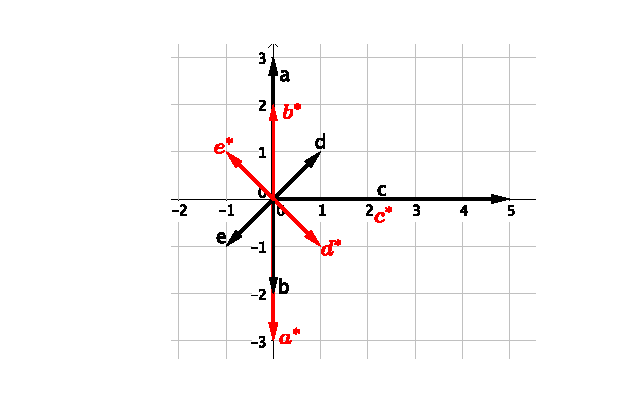
\includegraphics [width=0.44\textwidth ]{img-sol/t4-1a}\par Operacions:\par 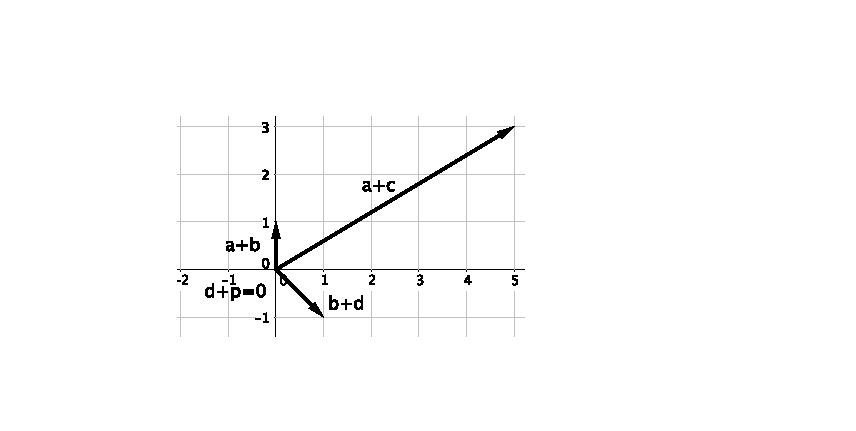
\includegraphics [width=0.44\textwidth ]{img-sol/t4-1b}
 \end{enumerate}
\vspace{0.3cm}

 \needspace{4\baselineskip} 

{\textbf{\em Pàgina 48}} \hrulefill
\begin{enumerate}
\vspace{0.25cm}


 \needspace{2\baselineskip} 

 \item[\fontfamily{phv}\selectfont\color{blue}\textbf{2}. ]  \scalebox{0.6}{\simbolclau } 
 \begin{tasks}[column-sep=1em, item-indent=1.3333em](2)
	 \task  $5 -9i$
	 \task $-6-15i$
	 \task $-13+11i$
	 \task 0
	 \task 13
	 \task $4 + 10i$
	 \task $2i$
	 \task $-4$
\end{tasks}
 \end{enumerate}
\begin{enumerate}
\vspace{0.25cm}


 \needspace{2\baselineskip} 

 \item[\fontfamily{phv}\selectfont\color{blue}\textbf{3}. ]  \scalebox{0.6}{\simbolclau } 
 \begin{tasks}[column-sep=1em, item-indent=1.3333em](2)
	 \task*  $-{{1}\over {10}}-{{7\,i}\over {10}}$
	 \task* $-{{11}\over {6}}+{{i}\over {2}}$
	 \task* ${{2}\over {5}}-{{i}\over {5}}$
	 \task ${{34\,i}\over {5}}$
\end{tasks}
\vspace{0.25cm}
\item[\fontfamily{phv}\selectfont\color{blue}\textbf{5. }] 
Racionalitzant el nombre s'expressa com $\dfrac {3a-1}{10}+\dfrac {a+3}{10}i$. Si igualam les parts real i imaginària, això passa si $3a-1=a+3$, és a dir $a=2$
\vspace{0.25cm}


 \needspace{2\baselineskip} 

 \item[\fontfamily{phv}\selectfont\color{blue}\textbf{6}. ]  \scalebox{0.6}{\simbolclau } 
 \begin{tasks}[column-sep=1em, item-indent=1.3333em](1)
	 \task  $|z|=2$; $arg(z)=-30^\circ $
	 \task* $|z|=\sqrt {8}$; $arg(z)=225 = - 135^\circ $
	 \task $|z|=2$; $arg(z)=-60^\circ $
	 \task $|z|=4$; $arg(z)=-90^\circ $
\end{tasks}
 \end{enumerate}
\vspace{0.3cm}

 \needspace{4\baselineskip} 

{\textbf{\em Pàgina 49}} \hrulefill
\begin{enumerate}
\vspace{0.25cm}


 \needspace{2\baselineskip} 

 \item[\fontfamily{phv}\selectfont\color{blue}\textbf{7}. ] 
 \begin{tasks}[column-sep=1em, item-indent=1.3333em](1)
	 \task* $|z|=\sqrt {18}$; $arg(z)=135^\circ $
	 \task $|z|=3$; $arg(z)=180^\circ $
	 \task $|z|=3$; $arg(z)=270^\circ $
	 \task* $|z|=\sqrt {18}$; $arg(z)=-45^\circ $
\end{tasks}
 \end{enumerate}
\begin{enumerate}
\vspace{0.25cm}


 \needspace{2\baselineskip} 

 \item[\fontfamily{phv}\selectfont\color{blue}\textbf{8}. ] 
 \begin{tasks}[column-sep=1em, item-indent=1.3333em](2)
	 \task* $z=\frac {3}{4}(-\sqrt {3}+i)$; $arg(z)=150^\circ $
	 \task* $z=\frac {1}{2}(1-i)$; $arg(z)=-45^\circ $
	 \task* $z=\left [2_{-60^\circ }\right ]^7$; $arg(z)=-420^\circ =-60^\circ $
\end{tasks}
\vspace{0.25cm}


 \needspace{2\baselineskip} 

 \item[\fontfamily{phv}\selectfont\color{blue}\textbf{9}. ] 
 \begin{tasks}[column-sep=1em, item-indent=1.3333em](2)
	 \task $1_{90^\circ }$
	 \task $1_{270^\circ }$
	 \task $4\sqrt {2}_{45^\circ }$
	 \task $4_{180^\circ }$
\end{tasks}
\vspace{0.25cm}


 \needspace{2\baselineskip} 

 \item[\fontfamily{phv}\selectfont\color{blue}\textbf{10}. ] 
 \begin{tasks}[column-sep=1em, item-indent=1.3333em](2)
	 \task $5_{90^\circ }$
	 \task $7_{270^\circ }$
	 \task $5\sqrt {2}_{-45^\circ }$
	 \task $2_{30^\circ }$
\end{tasks}
\vspace{0.25cm}


 \needspace{2\baselineskip} 

 \item[\fontfamily{phv}\selectfont\color{blue}\textbf{11}. ]  \scalebox{0.6}{\simbolclau } 
 \begin{tasks}[column-sep=1em, item-indent=1.3333em](1)
	 \task*  $2_{\,60^\circ }= 1 - \sqrt {3} i$
	 \task* $3_{\,-45^\circ }= \frac {3\sqrt {2}}{2} - \frac {3\sqrt {2}}{2} i$
	 \task $1_{\,90^\circ }= i $
	 \task* $5_{\,120^\circ }= -\frac {5}{2} + i \frac {5\sqrt {3}}{2}$
\end{tasks}
 \end{enumerate}
\vspace{0.3cm}

 \needspace{4\baselineskip} 

{\textbf{\em Pàgina 50}} \hrulefill
\begin{enumerate}
\vspace{0.25cm}


 \needspace{2\baselineskip} 

 \item[\fontfamily{phv}\selectfont\color{blue}\textbf{12}. ] 
 \begin{tasks}[column-sep=1em, item-indent=1.3333em](1)
	 \task* $\dfrac {\sqrt {2} i}{-2-2i}=\dfrac {\sqrt {2}_{90}}{2\sqrt {2}_{-135}}=\dfrac {1}{2}_{225}=\dfrac {1}{2} (\cos 225 + i \sin 255)=-\dfrac {1}{4}(1+i)$
	 \task* $\left (\frac {1}{2} + \frac {\sqrt {3}i}{2}\right )^{30}=\left ( 1_{60^\circ } \right )^{30}= 1_{1800^\circ }=1$ 
\end{tasks}
 \end{enumerate}
\begin{enumerate}
\vspace{0.25cm}


 \needspace{2\baselineskip} 

 \item[\fontfamily{phv}\selectfont\color{blue}\textbf{13}. ] 
 \begin{tasks}[column-sep=1em, item-indent=1.3333em](1)
	 \task* $(\sqrt {3}+i)^{60}=(2_{30})^{60}=2^{60}_{1800}=2^{60}$
	 \task* $(4-4i)^{-11}=(4\sqrt {2}_{-45^\circ })^{-11}=\frac {1}{2^{27}\sqrt {2}}_{495}=\frac {1}{2^{27}\sqrt {2}}_{135}=\frac {1}{2^{27}\sqrt {2}}(\cos 135 + i \sin 135)=\frac {1}{2^{28}} (-1+i)$
	 \task* $\dfrac {(1-\sqrt {3} i)^{12}}{(-2-2i)^8}=\dfrac {(2_{-60^\circ })^{12}}{(2\sqrt {2}_{-135^\circ })^8}= \dfrac {2^{12}_{-720^\circ }}{2^{12}_{-1080^\circ }}=1_{360^\circ }=1$
\end{tasks}
\vspace{0.25cm}


 \needspace{2\baselineskip} 

 \item[\fontfamily{phv}\selectfont\color{blue}\textbf{14}. ] 
 \begin{tasks}[column-sep=1em, item-indent=1.3333em](1)
	 \task $\cos (-\theta )=\cos \theta $
	 \task* $\sin (-\theta )=-\sin \theta $
	 \task* $\cos 3\theta =\cos ^3 \theta - 3\sin ^2 \theta \cos \theta $
	 \task* $\sin 3\theta =3\sin \theta \cos ^2 \theta - \sin ^3\theta $
\end{tasks}
\vspace{0.25cm}


 \needspace{2\baselineskip} 

 \item[\fontfamily{phv}\selectfont\color{blue}\textbf{15}. ] 
 \begin{tasks}[column-sep=1em, item-indent=1.3333em](2)
	 \task* $\sqrt {-3 i} \rightarrow $ $z=\pm \frac {\sqrt {6}}{2}(1-i)$ \par 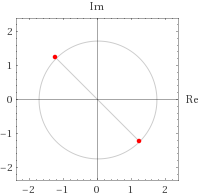
\includegraphics [width=0.3\textwidth ]{img-sol/t4-15a}
	 \task* $\sqrt {-9}\rightarrow $ $z=\pm 3i$ \par 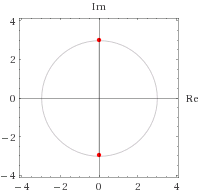
\includegraphics [width=0.3\textwidth ]{img-sol/t4-15b}
	 \task* $\sqrt {1+\sqrt {3} \,i}\rightarrow $ $z_1=\pm \frac {1}{2}(\sqrt {6}+i\sqrt {2})$ \par 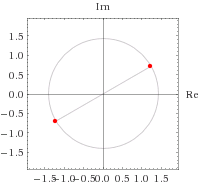
\includegraphics [width=0.3\textwidth ]{img-sol/t4-15c}
	 \task* $\sqrt [3]{-27}\rightarrow $ $z_1=-3$; $z_2=\frac {3}{2}(1+i\sqrt {3})$; $z_3=\frac {3}{2}(1-i\sqrt {3})$ \par 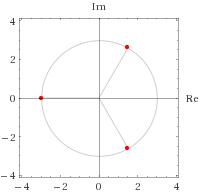
\includegraphics [width=0.3\textwidth ]{img-sol/t4-15d}
	 \task* $\sqrt [3]{1-i}\rightarrow $ $z_1\approx 1.084-0.29i$; $z_2 \approx -0.29 +1.084i$; $z_3=-0.794-0.794i$ \par 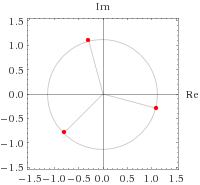
\includegraphics [width=0.3\textwidth ]{img-sol/t4-15e}
	 \task* $\sqrt [4]{-81}\rightarrow $ $z=\pm \frac {3\sqrt {2}}{2}(1+i)$; $z=\pm \frac {3\sqrt {2}}{2}(1-i)$\par 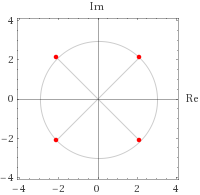
\includegraphics [width=0.3\textwidth ]{img-sol/t4-15f}
\end{tasks}
 \end{enumerate}
\vspace{0.3cm}

 \needspace{4\baselineskip} 

{\textbf{\em Pàgina 51}} \hrulefill
\begin{enumerate}
\vspace{0.25cm}


 \needspace{2\baselineskip} 

 \item[\fontfamily{phv}\selectfont\color{blue}\textbf{16}. ] 
 \begin{tasks}[column-sep=1em, item-indent=1.3333em](1)
	 \task* $\sqrt [5]{1} \rightarrow $ $z= 1$; $z \approx 0.309 \pm 0.9511i$; $z\approx -0.809\pm 0.5878 i$ \par 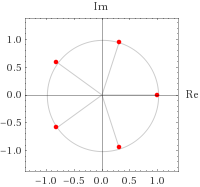
\includegraphics [width=0.3\textwidth ]{img-sol/t4-16a}
	 \task* $\sqrt [5]{-1} \rightarrow $ $z=-1 $; $z \approx 0.809\pm 0.588 i$; $z=-0.309 \pm 0.9511 i$ \par 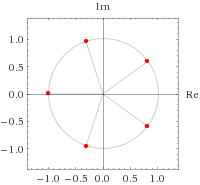
\includegraphics [width=0.3\textwidth ]{img-sol/t4-16b}
\end{tasks}
 \end{enumerate}
\begin{enumerate}
\vspace{0.25cm}


 \needspace{2\baselineskip} 

 \item[\fontfamily{phv}\selectfont\color{blue}\textbf{17}. ] 
 \begin{tasks}[column-sep=1em, item-indent=1.3333em](1)
	 \task $x=\sqrt [3]{-27}$ exemple
	 \task* $x=\sqrt [4]{-81}$ exercici anterior f)
	 \task* $x=\sqrt [5]{-32}\rightarrow $ $z=-2$; $z\approx 1.618 \pm 1.1756 i$; $z=-0.618 \pm 1.9021 i$; \par 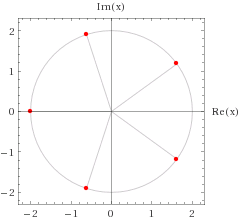
\includegraphics [width=0.3\textwidth ]{img-sol/t4-17c}
	 \task* $x=\sqrt [3]{8}\rightarrow $ $z=2$; $z=-1\pm \sqrt {3}i$;\par 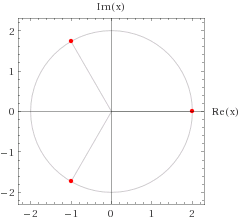
\includegraphics [width=0.3\textwidth ]{img-sol/t4-17d} 
\end{tasks}
\vspace{0.25cm}


 \needspace{2\baselineskip} 

 \item[\fontfamily{phv}\selectfont\color{blue}\textbf{18}. ] 
 \begin{tasks}[column-sep=1em, item-indent=1.3333em](1)
	 \task $x^2=-1\rightarrow $ $z=\pm i$
	 \task* $x^3=-8 \rightarrow $ $z=-2$; $z=1+\sqrt {3}i$; $z=1-\sqrt {3}i$
	 \task* $x^4+16=0 \rightarrow $ $z=\pm 2$; $z=\pm 2i$
\end{tasks}
\vspace{0.25cm}


 \needspace{2\baselineskip} 

 \item[\fontfamily{phv}\selectfont\color{blue}\textbf{19}. ] 
 \begin{tasks}[column-sep=1em, item-indent=1.3333em](1)
	 \task* $\sqrt {1} \rightarrow $ $z=\pm 1$
	 \task* $\sqrt [3]{1} \rightarrow $ $z=1$; $z=\frac {1}{2}(-1\pm \sqrt {3})$ \par 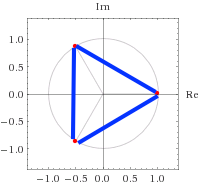
\includegraphics [width=0.3\textwidth ]{img-sol/t4-19b}
	 \task* $\sqrt {4} \rightarrow $ $z=\pm 1$; $z=\pm i$ \par 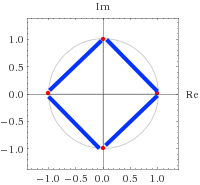
\includegraphics [width=0.3\textwidth ]{img-sol/t4-19c}
\end{tasks}
\vspace{0.25cm}
\item[\fontfamily{phv}\selectfont\color{blue}\textbf{20. }] 
Dues arrels reals: $z=\dfrac {-3\pm \sqrt {13}}{2}$
\vspace{0.25cm}


 \needspace{2\baselineskip} 

 \item[\fontfamily{phv}\selectfont\color{blue}\textbf{21}. ] 
 \begin{tasks}[column-sep=1em, item-indent=1.3333em](1)
	 \task* $z=\sqrt [6]{-64}$; $z=\pm 2i$; $z=\pm (\sqrt {3}+i)$; $z=\pm (\sqrt {3}-i)$
	 \task* $-3z^4+10z^3-10z+3=-(z-3)(z-1)(z+1)(3z-1)$ té solucions reals $z=3$; $z=\pm 1$; $z=1/3$
	 \task* Identificam una progressió geomètrica de raó $z$: La seva suma\par $\dfrac {z^7-1}{z-1}=0$ implica que $z^7=1$; són les arrels setenes de 1 (1 no serveix): Totes les arrels són per tant complexes: $z=-0.9 \pm 0.434 i$; $z=-0.22\pm 0.975 i$; $z=0.623 \pm 0.782$
\end{tasks}
\vspace{0.25cm}


 \needspace{2\baselineskip} 

 \item[\fontfamily{phv}\selectfont\color{blue}\textbf{22}. ] 
 \begin{tasks}[column-sep=1em, item-indent=1.3333em](2)
	 \task* Veure exemple;\par 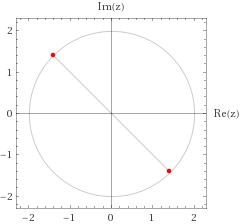
\includegraphics [width=0.3\textwidth ]{img-sol/t4-22a}
	 \task* $z=2i$; $z=-\sqrt {3}-i$; $z=\sqrt {3}-i$;\par 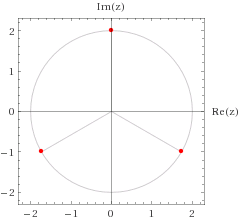
\includegraphics [width=0.3\textwidth ]{img-sol/t4-22b}
	 \task* $z=3i$; $z=-\frac {3}{2}(\sqrt {3}+i)$; $z=\frac {3}{2}(\sqrt {3}-i)$;\par 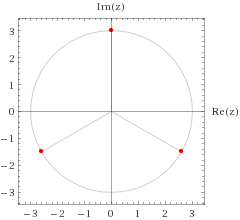
\includegraphics [width=0.3\textwidth ]{img-sol/t4-22c}
	 \task* $z=\pm (1.3066+0.5412 i)$; $z=\pm (0.5412-1.3055 i)$;\par 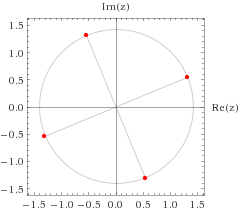
\includegraphics [width=0.3\textwidth ]{img-sol/t4-22d} 
\end{tasks}
 \end{enumerate}
\vspace{0.3cm}

 \needspace{4\baselineskip} 

{\textbf{\em Pàgina 52}} \hrulefill
\begin{enumerate}
\vspace{0.25cm}
 \item[$\bullet$ ] {\fontfamily{phv}\selectfont\color{blue}\textbf{Autoavaluació:}. }

 \end{enumerate}
\begin{enumerate}
\vspace{0.25cm}


 \needspace{2\baselineskip} 

 \item[\fontfamily{phv}\selectfont\color{blue}\textbf{1}. ]  \scalebox{0.6}{\simbolclau } 
 \begin{tasks}[column-sep=1em, item-indent=1.3333em](2)
	 \task $-5-6i$
	 \task $-8-6i$
	 \task $10i$
	 \task $-2+i$
\end{tasks}
\vspace{0.25cm}
\item[\fontfamily{phv}\selectfont\color{blue}\textbf{2. }]  \scalebox{0.6}{\simbolclau } 
$-46+63i$
\vspace{0.25cm}
\item[\fontfamily{phv}\selectfont\color{blue}\textbf{3. }]  \scalebox{0.6}{\simbolclau } 
$z_1=5+2i$, $z_2=5-2i$
\vspace{0.25cm}


 \needspace{2\baselineskip} 

 \item[\fontfamily{phv}\selectfont\color{blue}\textbf{4}. ]  \scalebox{0.6}{\simbolclau } 
 \begin{tasks}[column-sep=1em, item-indent=1.3333em](2)
	 \task Real $k=-2$
	 \task Imaginari pur $k=-2$
\end{tasks}
\vspace{0.25cm}
\item[\fontfamily{phv}\selectfont\color{blue}\textbf{5. }]  \scalebox{0.6}{\simbolclau } 
$x=\pm 2$
\vspace{0.25cm}
\item[\fontfamily{phv}\selectfont\color{blue}\textbf{6. }]  \scalebox{0.6}{\simbolclau } 
$3\sqrt {2}$, $3\pi /4$
\vspace{0.25cm}
\item[\fontfamily{phv}\selectfont\color{blue}\textbf{7. }]  \scalebox{0.6}{\simbolclau } 
$1+\sqrt {3}i$
\vspace{0.25cm}
\item[\fontfamily{phv}\selectfont\color{blue}\textbf{8. }]  \scalebox{0.6}{\simbolclau } 
$-8i$
\vspace{0.25cm}
\item[\fontfamily{phv}\selectfont\color{blue}\textbf{9. }]  \scalebox{0.6}{\simbolclau } 
$5(\cos (\pi /2) +i \sin (\pi /2)$
\vspace{0.25cm}
\item[\fontfamily{phv}\selectfont\color{blue}\textbf{10. }]  \scalebox{0.6}{\simbolclau } 
$z_1=2_{110^\circ }$, $z_2=2_{230^\circ }$, $z_3=2_{350^\circ }$
 \end{enumerate}
\vfill\null
\columnbreak
\def\currentname{Solucions del Bloc I}
\vspace*{0.75cm}

 
 \needspace{5\baselineskip} 
 \scalebox{1.25}{\heading{Solucions del Bloc I}}

\vspace*{0.4cm}
\phantomsection \addcontentsline{toc}{section}{Solucions del Bloc I}
\vspace{0.3cm}

 \needspace{4\baselineskip} 

{\textbf{\em Pàgina 54}} \hrulefill
\begin{enumerate}
\vspace{0.25cm}
\item[\fontfamily{phv}\selectfont\color{blue}\textbf{1. }]  \scalebox{0.6}{\simbolclau } 
a) $a\sqrt {a}$ \quad \quad b) $\frac {3\sqrt {2}-4\sqrt {6}}{6}$
 \end{enumerate}
\begin{enumerate}
\vspace{0.25cm}
\item[\fontfamily{phv}\selectfont\color{blue}\textbf{2. }]  \scalebox{0.6}{\simbolclau } 
a) $a\,\sqrt [20]{a}$ \quad \quad b)$\frac {2\sqrt {3}+3\sqrt {2}-6}{6}$
\vspace{0.25cm}
\item[\fontfamily{phv}\selectfont\color{blue}\textbf{3. }]  \scalebox{0.6}{\simbolclau } 
$x^2 (x+1) (x-2) (3x-1)$
\vspace{0.25cm}
\item[\fontfamily{phv}\selectfont\color{blue}\textbf{4. }]  \scalebox{0.6}{\simbolclau } 
2
\vspace{0.25cm}
\item[\fontfamily{phv}\selectfont\color{blue}\textbf{5. }]  \scalebox{0.6}{\simbolclau } 
$x=3$ vàlida.
\vspace{0.25cm}
\item[\fontfamily{phv}\selectfont\color{blue}\textbf{6. }]  \scalebox{0.6}{\simbolclau } 
$x=1$
\vspace{0.25cm}
\item[\fontfamily{phv}\selectfont\color{blue}\textbf{7. }]  \scalebox{0.6}{\simbolclau } 
$(3, +\infty )$
\vspace{0.25cm}
\item[\fontfamily{phv}\selectfont\color{blue}\textbf{8. }]  \scalebox{0.6}{\simbolclau } 
$x=38$: be, $y=18$: malament, $z=4$: no contestades. Planteig: $x+y+z=60$; $5x-2y-z=150$; $y+5z=x$
\vspace{0.25cm}
\item[\fontfamily{phv}\selectfont\color{blue}\textbf{9. }]  \scalebox{0.6}{\simbolclau } 
S.C.I. $x=1$, $y=z-3$, $z=z$
 \end{enumerate}
\vspace{0.3cm}

 \needspace{4\baselineskip} 

{\textbf{\em Pàgina 55}} \hrulefill
\begin{enumerate}
\vspace{0.25cm}
\item[\fontfamily{phv}\selectfont\color{blue}\textbf{10. }]  \scalebox{0.6}{\simbolclau } 
Els costats són 10.49 cm i 20.25 cm, el perímetre 61.48 cm. L'àrea 83.23 cm$^2$.
 \end{enumerate}
\begin{enumerate}
\vspace{0.25cm}
\item[\fontfamily{phv}\selectfont\color{blue}\textbf{11. }]  \scalebox{0.6}{\simbolclau } 
Primer obtenim els costats resolent un sistema d'equacions $a=19$, $b=16$ i $c=13$. Després aplicam el Teorema del Cosinus per obtenir els angles $\hat A=42.54^\circ $, $\hat B=56.3^\circ $, $\hat C=81.17^\circ $
\vspace{0.25cm}
\item[\fontfamily{phv}\selectfont\color{blue}\textbf{12. }]  \scalebox{0.6}{\simbolclau } 
Utilitzam el Teorema del Sinus. $\hat C= 56^\circ \, 19^\prime \, 31^{\prime \prime }$, $\hat B= 51^\circ \, 40^\prime \, 29^{\prime \prime }$ i $\bar {AC}=263.96$ m.
\vspace{0.25cm}
\item[\fontfamily{phv}\selectfont\color{blue}\textbf{13. }]  \scalebox{0.6}{\simbolclau } 
$d=3557$ km sobre la superfície de la Terra.
\vspace{0.25cm}
\item[\fontfamily{phv}\selectfont\color{blue}\textbf{14. }]  \scalebox{0.6}{\simbolclau } 
No existeix cap angle amb aquestes condicions. S'obtindria que $\cos a = 3/4$ i amb aquesta dada no es compleix que $\sin ^2 a +\cos ^2 a = 1$.
\vspace{0.25cm}
\item[\fontfamily{phv}\selectfont\color{blue}\textbf{15. }]  \scalebox{0.6}{\simbolclau } 
En primer lloc trobam que $\sin \alpha = \frac {2\sqrt 5}{5}$ i $\cos \alpha = \frac {\sqrt 5}{5}$. a) $-3/5$ \quad b) $\frac {\sqrt 5}{5}$ \quad c) $\sqrt {\frac {5-\sqrt 5}{10}}$ \quad d) $-3$
\vspace{0.25cm}
\item[\fontfamily{phv}\selectfont\color{blue}\textbf{16. }]  \scalebox{0.6}{\simbolclau } 
a) Utilitza que $sin^4 x = (1-\cos ^2 x)^2$ desenvolupa el quadrat i simplifica. b) Utilitza que $\cos ^2 \frac {\beta }{2} = \frac {1+\cos \beta }{2}$ 
\vspace{0.25cm}
\item[\fontfamily{phv}\selectfont\color{blue}\textbf{17. }]  \scalebox{0.6}{\simbolclau } 
a) $x= 0^\circ + n\cdot 360^\circ $, $x=126.87^\circ + n\cdot 360^\circ $. b) $x= 90^\circ + n\cdot 180^\circ $, $x= 60^\circ + n\cdot 360^\circ $, $x= 300^\circ + n\cdot 360^\circ $.
\vspace{0.25cm}
\item[\fontfamily{phv}\selectfont\color{blue}\textbf{18. }]  \scalebox{0.6}{\simbolclau } 
$x=30^\circ + n\cdot 180^\circ $, $y=30^\circ + k\cdot 180^\circ $.
\vspace{0.25cm}
\item[\fontfamily{phv}\selectfont\color{blue}\textbf{19. }]  \scalebox{0.6}{\simbolclau } 
$-\frac {19}{10}+\frac {37}{10}i$
\vspace{0.25cm}
\item[\fontfamily{phv}\selectfont\color{blue}\textbf{20. }]  \scalebox{0.6}{\simbolclau } 
$i$
\vspace{0.25cm}
\item[\fontfamily{phv}\selectfont\color{blue}\textbf{21. }]  \scalebox{0.6}{\simbolclau } 
$z=5+2i$, $z=5-2i$
\vspace{0.25cm}
\item[\fontfamily{phv}\selectfont\color{blue}\textbf{22. }]  \scalebox{0.6}{\simbolclau } 
 $z^*=3_{\, 300^\circ }$, $1/z=(1/3)_{\, 300^\circ }$, $z^2=9_{\, 120^\circ }$, $\sqrt [3]{z}$ té tres resultats = $(\sqrt {3})_{\, 20^\circ }$, $(\sqrt {3})_{\, 140^\circ }$ i $(\sqrt {3})_{\, 260^\circ }$.
 \end{enumerate}
\vfill\null
\columnbreak
\def\currentname{Solucions del Tema 5}
\vspace*{0.75cm}

 
 \needspace{5\baselineskip} 
 \scalebox{1.25}{\heading{Solucions del Tema 5}}

\vspace*{0.4cm}
\phantomsection \addcontentsline{toc}{section}{Solucions del Tema 5}
\vspace{0.3cm}

 \needspace{4\baselineskip} 

{\textbf{\em Pàgina 59}} \hrulefill
\begin{enumerate}
\vspace{0.25cm}
 \item[$\bullet$ ] {\fontfamily{phv}\selectfont\color{blue}\textbf{Avaluació inicial}. }
 \begin{tasks}(4) \task L$_{4}$ \task R$_3$ \task L$_2$ \task C$_4$ \task PI$_{2}$ \task E$_3$ \task C$_1$ \task E$_1$ \task L$_{1}$ \task PI$_4$ \task PI$_3$ \task R$_2$ \end{tasks} \par No tenen gràfica associada L$_3$, C$_2$, C$_3$, PI$_1$, R$_1$, R$_4$, E$_2$ i E$_4$. 
 \end{enumerate}
\vspace{0.3cm}

 \needspace{4\baselineskip} 

{\textbf{\em Pàgina 60}} \hrulefill
\begin{enumerate}
\vspace{0.25cm}
\item[\fontfamily{phv}\selectfont\color{blue}\textbf{1. }]  \scalebox{0.6}{\simbolclau } 
2, 3, 5, 8, 13, 21, 34, ...
 \end{enumerate}
\begin{enumerate}
\vspace{0.25cm}
\item[\fontfamily{phv}\selectfont\color{blue}\textbf{2. }]  \scalebox{0.6}{\simbolclau } 
a) $a_n=3+5(n-1)$ o $a_1=3$ $a_n=a_{n-1}+3$ \par b) $a_n=n^3$ \par c) $a_n=8\cdot (1/2)^{n-1}$ o $a_1=8$ $a_n=a_{n-1}/2$]
\vspace{0.25cm}
\item[\fontfamily{phv}\selectfont\color{blue}\textbf{3. }]  \scalebox{0.6}{\simbolclau } 
$a_n=10-3(n-1)$ i $a_{100}=-197$
\vspace{0.25cm}
\item[\fontfamily{phv}\selectfont\color{blue}\textbf{4. }]  \scalebox{0.6}{\simbolclau } 
$d=(19-11)/2=4$ i $a_1=3$, \linebreak $a_n=3+4(n-1)$, $S_{100}=20100$
\vspace{0.25cm}
\item[\fontfamily{phv}\selectfont\color{blue}\textbf{5. }]  \scalebox{0.6}{\simbolclau } 
$a_n=100\cdot (0.5)^{n-1}$, $a_{50}=1.776\cdot 10^{-13}$, $S_\infty =200$
\vspace{0.25cm}
\item[\fontfamily{phv}\selectfont\color{blue}\textbf{6. }]  \scalebox{0.6}{\simbolclau } 
$r=3$ i $a_1=1$, $a_n=3^{n-1}$, $S_{30}=1.029\cdot 10^{14}$
\vspace{0.25cm}
\item[\fontfamily{phv}\selectfont\color{blue}\textbf{7. }] 
Són funcions 2 i 4. No són funcions 1 i 3, perquè per un mateix valor de $x$ trobam més d'un valor de $y$ ``La gràfica té plegaments''.
 \end{enumerate}
\vspace{0.3cm}

 \needspace{4\baselineskip} 

{\textbf{\em Pàgina 61}} \hrulefill
\begin{enumerate}
\vspace{0.25cm}


 \needspace{2\baselineskip} 

 \item[\fontfamily{phv}\selectfont\color{blue}\textbf{8}. ] 
 \begin{tasks}[column-sep=1em, item-indent=1.3333em](1)
	 \task Dom $f=[-4,4]$
	 \task Dom $f=(-\infty ,3)]$
	 \task Dom $f=(-\infty ,-2)\cup (-2,2)\cup (2,+\infty )$ o també Dom $f=\Re -\{-2,2\}$
	 \task Dom $f=[-2,5]$
\end{tasks}
 \end{enumerate}
\vspace{0.3cm}

 \needspace{4\baselineskip} 

{\textbf{\em Pàgina 62}} \hrulefill
\begin{enumerate}
\vspace{0.25cm}
\item[\fontfamily{phv}\selectfont\color{blue}\textbf{9. }]  \scalebox{0.6}{\simbolclau } 
$\text {Dom }f=\Re -\{\pm 2\}$,\par $\text {Dom } g=(-\infty ,-2/3]\cup (3,+\infty )$,\par $\text {Dom } h=\Re -\{1\}$,\par $\text {Dom } i=\Re -\{\pm 1\}$,\par $\text {Dom } j=(-\infty ,-3]\cup (3,+\infty )$,\par $\text {Dom } k=\Re -\{\pm \sqrt {3}\}$,\par $\text {Dom } l=[-2,3)$, $\text {Dom } m=\Re - \{1\}$
 \end{enumerate}
\begin{enumerate}
\vspace{0.25cm}
\item[\fontfamily{phv}\selectfont\color{blue}\textbf{10. }] 
Dom $p=\Re $;\par Dom $q=\Re $;\par Dom $r=(-\infty ,-1]$;\par Dom $s=\Re $;\par Dom $f=\Re -\{-3\}$;\par Dom $g=\Re -\{0\}$;\par Dom $h=\Re $;\par Dom $j=\Re -\{-2,2\}$ 
\vspace{0.25cm}
\item[\fontfamily{phv}\selectfont\color{blue}\textbf{11. }] 
Si és senar $a=0$ i $c=0$. Si passa per $(1,-2)$ implica que $b=-3$
\vspace{0.25cm}
\item[\fontfamily{phv}\selectfont\color{blue}\textbf{12. }] 
Gràfica:\par 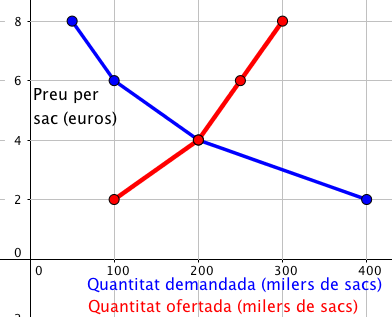
\includegraphics [width=0.4\textwidth ]{img-sol/t5-12}
 \end{enumerate}
\vspace{0.3cm}

 \needspace{4\baselineskip} 

{\textbf{\em Pàgina 63}} \hrulefill
\begin{enumerate}
\vspace{0.25cm}
\item[\fontfamily{phv}\selectfont\color{blue}\textbf{13. }] 
a) Gràfica:\par 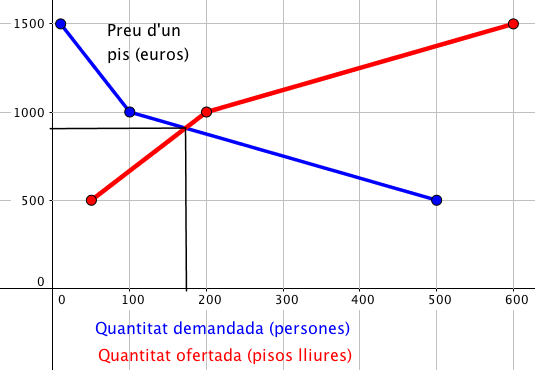
\includegraphics [width=0.4\textwidth ]{img-sol/t5-13}\par b) El punt d'equilibri és quan l'oferta iguala la demanda. Això passarà per una oferta de 175 pisos un preu per pis de 910 \euro {}.
 \end{enumerate}
\begin{enumerate}
\vspace{0.25cm}
\item[\fontfamily{phv}\selectfont\color{blue}\textbf{14. }] 
Gràfica: \par 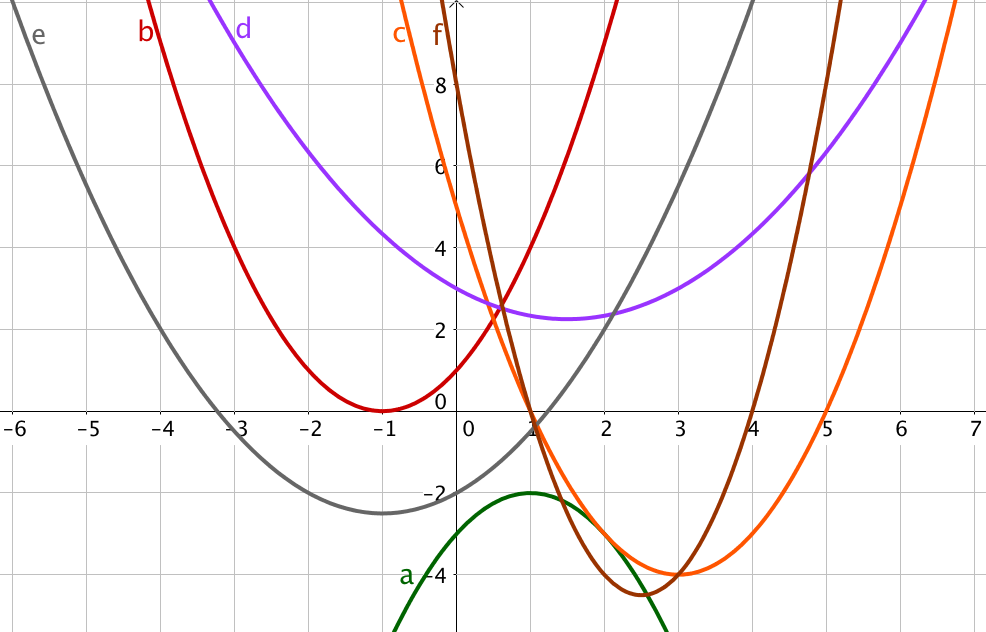
\includegraphics [width=0.4\textwidth ]{img-sol/t5-14}
\vspace{0.25cm}
\item[\fontfamily{phv}\selectfont\color{blue}\textbf{15. }] 
L'objecte es llança des d'una altura de 5 m. Al cap d'1 s està a 8 m. Assoleix una altura màxima de 9 m als 2 s. Arriba al terra als 5 segons.\par 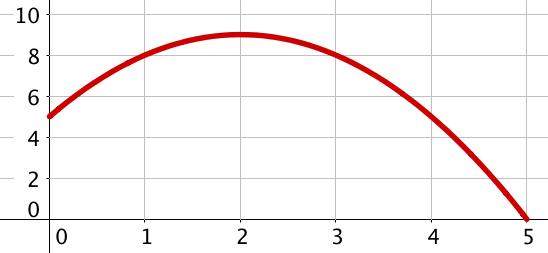
\includegraphics [width=0.4\textwidth ]{img-sol/t5-15}
\vspace{0.25cm}
\item[\fontfamily{phv}\selectfont\color{blue}\textbf{16. }] 
a) \par 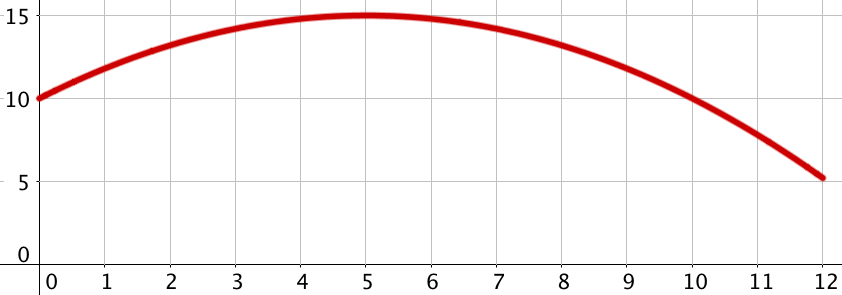
\includegraphics [width=0.4\textwidth ]{img-sol/t5-16} \par b) $f(6)=14.8$ i $f(12)=5.2$ cèntims.
\vspace{0.25cm}
\item[\fontfamily{phv}\selectfont\color{blue}\textbf{17. }] 
\mbox {}\par 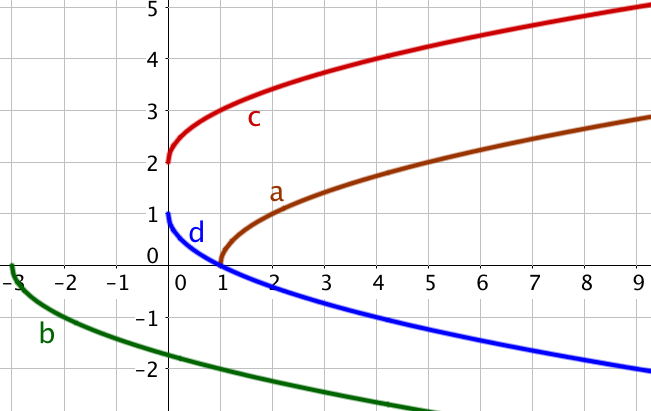
\includegraphics [width=0.4\textwidth ]{img-sol/t5-17}
 \end{enumerate}
\vspace{0.3cm}

 \needspace{4\baselineskip} 

{\textbf{\em Pàgina 64}} \hrulefill
\begin{enumerate}
\vspace{0.25cm}
\item[\fontfamily{phv}\selectfont\color{blue}\textbf{18. }] 
\mbox {}\par 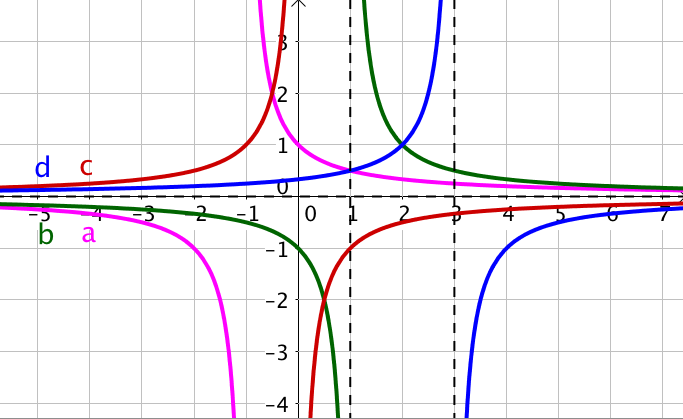
\includegraphics [width=0.4\textwidth ]{img-sol/t5-18}
 \end{enumerate}
\begin{enumerate}
\vspace{0.25cm}
\item[\fontfamily{phv}\selectfont\color{blue}\textbf{19. }] 
\mbox {}\par 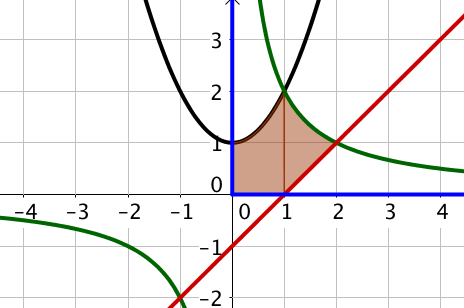
\includegraphics [width=0.4\textwidth ]{img-sol/t5-19}
\vspace{0.25cm}
\item[\fontfamily{phv}\selectfont\color{blue}\textbf{20. }] 
Dom $f=[0,+\infty ]$. Tall eix OX $(2,0)$; Tall eix OY $(0,-20)$. No presenta simetries. La funció és negativa a $[0,2)$ i positiva a $(2,+\infty )$.
\vspace{0.25cm}
\item[\fontfamily{phv}\selectfont\color{blue}\textbf{21. }] 
$|x|=\left \{ \begin {array}{ll} -x & \text { si } x<0 \\ x & \text { si } x\ge 0 \end {array} \right .$
\vspace{0.25cm}
\item[\fontfamily{phv}\selectfont\color{blue}\textbf{22. }] 
\mbox {}\par 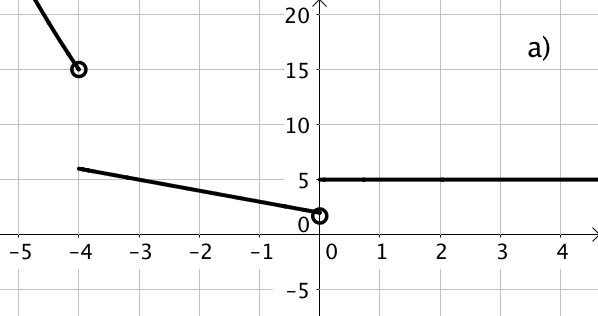
\includegraphics [width=0.4\textwidth ]{img-sol/t5-22a}\par \includegraphics [width=0.4\textwidth ]{img-sol/t5-22b}
\vspace{0.25cm}
\item[\fontfamily{phv}\selectfont\color{blue}\textbf{23. }] 
\mbox {}\par \includegraphics [width=0.4\textwidth ]{img-sol/t5-23}
\vspace{0.25cm}
\item[\fontfamily{phv}\selectfont\color{blue}\textbf{24. }] 
\mbox {}\par \includegraphics [width=0.4\textwidth ]{img-sol/t5-24}
\vspace{0.25cm}
\item[\fontfamily{phv}\selectfont\color{blue}\textbf{25. }] 
\mbox {}\par \includegraphics [width=0.4\textwidth ]{img-sol/t5-25}
\vspace{0.25cm}
\item[\fontfamily{phv}\selectfont\color{blue}\textbf{26. }] 
\mbox {}\par \includegraphics [width=0.4\textwidth ]{img-sol/t5-26}
 \end{enumerate}
\vspace{0.3cm}

 \needspace{4\baselineskip} 

{\textbf{\em Pàgina 65}} \hrulefill
\begin{enumerate}
\vspace{0.25cm}
\item[\fontfamily{phv}\selectfont\color{blue}\textbf{28. }] 
\mbox {}\par \includegraphics [width=0.4\textwidth ]{img-sol/t5-28}
 \end{enumerate}
\begin{enumerate}
\vspace{0.25cm}
\item[\fontfamily{phv}\selectfont\color{blue}\textbf{29. }] 
Són simètriques respecte l'eix OY.
\vspace{0.25cm}


 \needspace{2\baselineskip} 

 \item[\fontfamily{phv}\selectfont\color{blue}\textbf{30}. ] 
 \begin{tasks}[column-sep=1em, item-indent=1.3333em](2)
	 \task* \mbox {}\par \begin {tabular}{|c|c|c|c|c|c|c|} anys & 1 & 2 & 3 & 4 & 5 & 10 \\ \hline k\euro {} & 5.1 & 5.202 & 5.306 & 5.41 & 5.52 & 6.09 \end {tabular}
	 \task $C=5\cdot 1.02^x$ 
\end{tasks}
\vspace{0.25cm}
\item[\fontfamily{phv}\selectfont\color{blue}\textbf{31. }] 
$y=10\cdot \left (\frac {1}{3}\right )^x$, $x$ hores passades des de les 9 del matí. A les 3 del matí $y(-6)=7290$ i a les 12 del migdia $y(3)=0.37$ milions.
 \end{enumerate}
\vspace{0.3cm}

 \needspace{4\baselineskip} 

{\textbf{\em Pàgina 66}} \hrulefill
\begin{enumerate}
\vspace{0.25cm}


 \needspace{2\baselineskip} 

 \item[\fontfamily{phv}\selectfont\color{blue}\textbf{32}. ] 
 \begin{tasks}[column-sep=1em, item-indent=1.3333em](2)
	 \task* $f\circ h=2^{-3x+3}-3\,2^{-2x+2}+3\,2^{-x+1}-1$;\par $g\circ h=\sqrt {\frac {2^{-x+1}-2}{2^{-x+1}+7}}$;\par $g\circ j=\sqrt {\frac {\ln (x^5-1)-2}{\ln (x^5-1)+7}}$;\par $k\circ h=2^{2^{-x+1}}\cdot 30^{2^{-x+1}-1}$;\par $g\circ h \circ j=\sqrt {\frac {2^{-\ln (x^5-1)+1}-2}{2^{-\ln (x^5-1)+1}+7}}$;\par $m\circ j=\sqrt [4]{-5+2\ln (x^5-1)}$
	 \task* Dom $f=\Re $; Dom $g=(-\infty ,-7)\cup [2,+\infty ]$; Dom $h=\Re $; Dom $j=(1,+\infty )$; Dom $k=\Re $; Dom $m=[5/2,+\infty ]$
\end{tasks}
 \end{enumerate}
\begin{enumerate}
\vspace{0.25cm}
\item[\fontfamily{phv}\selectfont\color{blue}\textbf{33. }]  \scalebox{0.6}{\simbolclau } 
$p^{-1}=(3-x)/5$,\par $q^{-1}=\pm \sqrt {(x+1)/2}$,\par $r^{-1}=\sqrt [3]{6-x}$, $s^{-1}=-x$,\par $f^{-1}=(3x+4)/(2-x)$, $g^{-1}=-3/x$,\par $h^{-1}=(1\pm \sqrt {1+4x})/2$,\par $j^{-1}=\pm \sqrt {4x/(1+x)}$, \,\,$k^{-1}=4+\ln x$,\par $l^{-1}=1/\log _2 {x}$,\par $m^{-1}=\log x /(\log 2 - \log 3)$,\par $n^{-1}=\ln x / (\ln x -1)$,\par $a^{-1}=2+e^x$, $b^{-1}=3\cdot 10^x +1$,\par $c^{-1}=(1+4 e^x)/(1-2 e^x)$,\par $d^{-1}=\sqrt [3]{1+10^x}$ 
\vspace{0.25cm}
\item[\fontfamily{phv}\selectfont\color{blue}\textbf{34. }] 
La funció representada és la recta $y=-\frac {3}{5}x+3$. La seva inversa és $y=-\frac {5}{3}x+5$
 \end{enumerate}
\vspace{0.3cm}

 \needspace{4\baselineskip} 

{\textbf{\em Pàgina 67}} \hrulefill
\begin{enumerate}
\vspace{0.25cm}


 \needspace{2\baselineskip} 

 \item[\fontfamily{phv}\selectfont\color{blue}\textbf{35}. ] 
 \begin{tasks}[column-sep=1em, item-indent=1.3333em](2)
	 \task $x=5$
	 \task $x=3$
	 \task $x=\frac {1}{2}$
	 \task $x=4$
	 \task $x=5$
	 \task $x=\frac {1}{16}$
\end{tasks}
 \end{enumerate}
\begin{enumerate}
\vspace{0.25cm}


 \needspace{2\baselineskip} 

 \item[\fontfamily{phv}\selectfont\color{blue}\textbf{36}. ] 
 \begin{tasks}[column-sep=1em, item-indent=1.3333em](2)
	 \task $x=\pm \frac {1}{10}$
	 \task $x=\log _7 115\approx 2,438$
	 \task* $x=\frac {\sqrt {7}}{3}\approx 0,882$
	 \task* $x=-2+\log _3 172\approx 2,685$
	 \task $x=e^2\approx 7,389$
	 \task $x=\frac {3}{2}$
\end{tasks}
\vspace{0.25cm}


 \needspace{2\baselineskip} 

 \item[\fontfamily{phv}\selectfont\color{blue}\textbf{37}. ]  \scalebox{0.6}{\simbolclau } 
 \begin{tasks}[column-sep=1em, item-indent=1.3333em](1)
	 \task $x=15$ ($x=0$ no vàlida)
	 \task $x=2$
	 \task $x=100$ ($x=0$ no vàlida)
	 \task $x=2/(\log 2 - 1)$
	 \task $x=12/5$
	 \task $x=1$ i $x=-2$
\end{tasks}
 \end{enumerate}
\vspace{0.3cm}

 \needspace{4\baselineskip} 

{\textbf{\em Pàgina 68}} \hrulefill
\begin{enumerate}
\vspace{0.25cm}


 \needspace{2\baselineskip} 

 \item[\fontfamily{phv}\selectfont\color{blue}\textbf{38}. ] 
 \begin{tasks}[column-sep=1em, item-indent=1.3333em](2)
	 \task $y=\log _4 x$
	 \task $y=\ln x$
	 \task $y=\log _{1/4} x=-\log _4 x$
	 \task $y=\log _{1/e} x=-\ln x$
\end{tasks}
 \end{enumerate}
\begin{enumerate}
\vspace{0.25cm}
\item[\fontfamily{phv}\selectfont\color{blue}\textbf{39. }] 
\mbox {}\par \includegraphics [width=0.4\textwidth ]{img-sol/t5-39}
\vspace{0.25cm}
\item[\fontfamily{phv}\selectfont\color{blue}\textbf{40. }] 
Dom $f=(0,+\infty )$
\vspace{0.25cm}
\item[\fontfamily{phv}\selectfont\color{blue}\textbf{41. }] 
Punt de tall $A(e,1)$ i $B(1/e,1)$ \par \includegraphics [width=0.4\textwidth ]{img-sol/t5-41}
\vspace{0.25cm}
\item[\fontfamily{phv}\selectfont\color{blue}\textbf{42. }] 
Dom $f=(0,+\infty )$; Dom $g=\Re $; Dom $h=\Re $
\vspace{0.25cm}
\item[\fontfamily{phv}\selectfont\color{blue}\textbf{43. }] 
\mbox {}\par \includegraphics [width=0.4\textwidth ]{img-sol/t5-43}
\vspace{0.25cm}
\item[\fontfamily{phv}\selectfont\color{blue}\textbf{44. }] 
\mbox {}\par \includegraphics [width=0.4\textwidth ]{img-sol/t5-44}
\vspace{0.25cm}
\item[\fontfamily{phv}\selectfont\color{blue}\textbf{45. }] 
\mbox {}\par \includegraphics [width=0.4\textwidth ]{img-sol/t5-45}
\vspace{0.25cm}
\item[\fontfamily{phv}\selectfont\color{blue}\textbf{46. }] 
\mbox {}\par \includegraphics [width=0.4\textwidth ]{img-sol/t5-46}
 \end{enumerate}
\vspace{0.3cm}

 \needspace{4\baselineskip} 

{\textbf{\em Pàgina 69}} \hrulefill
\begin{enumerate}
\vspace{0.25cm}
 \item[$\bullet$ ] {\fontfamily{phv}\selectfont\color{blue}\textbf{Autoavaluació:}. }

 \end{enumerate}
\begin{enumerate}
\vspace{0.25cm}
\item[\fontfamily{phv}\selectfont\color{blue}\textbf{1. }]  \scalebox{0.6}{\simbolclau } 
\textbf {-- 10.} Autoavaluació: 1a; 2d; 3d; 4b; 5c; 6b; 7b; 8a; 9c; 10c
 \end{enumerate}
\vfill\null
\columnbreak
\def\currentname{Solucions del Tema 6}
\vspace*{0.75cm}

 
 \needspace{5\baselineskip} 
 \scalebox{1.25}{\heading{Solucions del Tema 6}}

\vspace*{0.4cm}
\phantomsection \addcontentsline{toc}{section}{Solucions del Tema 6}
\vspace{0.3cm}

 \needspace{4\baselineskip} 

{\textbf{\em Pàgina 73}} \hrulefill
\begin{enumerate}
\vspace{0.25cm}
\item[\fontfamily{phv}\selectfont\color{blue}\textbf{1. }] 
$\limx {3^-} f_1(x)=-\infty $\par \begin {tabular}{|c|c|c|c|c|c|} \hline $x$ & 2 & 2,5 & 2,9 & 2,99 & 2,999 \\ \hline $f_1$ & -5 & -20 & -500 & $-5\cdot 10^4$& $-5\cdot 10^6$\\ \hline \end {tabular}\par $\limx {3^-} f_2(x)=+\infty $\par \begin {tabular}{|c|c|c|c|c|c|} \hline $x$ & 2 & 2,5 & 2,9 & 2,99 & 2,999 \\ \hline $f_2$ & 4 & 8& 40& 400& 4000 \\ \hline \end {tabular}\par $\limx {3^-} f_3(x)=8$\par \begin {tabular}{|c|c|c|c|c|c|} \hline $x$ & 2 & 2,5 & 2,9 & 2,99 & 2,999 \\ \hline $f_3$ & 4 & 5,66 & 7,46 & 7,94 & 7,99 \\ \hline \end {tabular} 
 \end{enumerate}
\begin{enumerate}
\vspace{0.25cm}


 \needspace{2\baselineskip} 

 \item[\fontfamily{phv}\selectfont\color{blue}\textbf{2}. ] 
 \begin{tasks}[column-sep=1em, item-indent=1.3333em](1)
	 \task*  $\limx {3} f(x)=\nexists $; $\limx {2} f(x)=1$; $\limx {+\infty } f(x)=0^-$; $\limx {-\infty } f(x)=+\infty $
	 \task* $\limx {3} f(x)=0$; $\limx {2} f(x)=\nexists $; $\limx {+\infty } f(x)=-\infty $; $\limx {-\infty } f(x)=3$ 
\end{tasks}
\vspace{0.25cm}


 \needspace{2\baselineskip} 

 \item[\fontfamily{phv}\selectfont\color{blue}\textbf{3}. ] 
 \begin{tasks}[column-sep=1em, item-indent=1.3333em](2)
	 \task* $\limx {1^-} f=1$; $\limx {1^+} f=1$
	 \task* $\limx {1^-} f=1/6$; $\limx {1^+} f=5/4$
	 \task* $\limx {0^-} f=-\infty $; $\limx {0^+} f=0$
	 \task* $\limx {5^-} f=10$; $\limx {5^+} f=10$
\end{tasks}
 \end{enumerate}
\vspace{0.3cm}

 \needspace{4\baselineskip} 

{\textbf{\em Pàgina 74}} \hrulefill
\begin{enumerate}
\vspace{0.25cm}


 \needspace{2\baselineskip} 

 \item[\fontfamily{phv}\selectfont\color{blue}\textbf{4}. ] 
 \begin{tasks}[column-sep=1em, item-indent=1.3333em](2)
	 \task $+\infty $
	 \task $-\infty $
	 \task $-\infty $
	 \task $+\infty $
\end{tasks}
 \end{enumerate}
\begin{enumerate}
\vspace{0.25cm}


 \needspace{2\baselineskip} 

 \item[\fontfamily{phv}\selectfont\color{blue}\textbf{5}. ]  \scalebox{0.6}{\simbolclau } 
 \begin{tasks}[column-sep=1em, item-indent=1.3333em](2)
	 \task --1/6
	 \task 0
	 \task --9
	 \task 1
	 \task --12
	 \task $\mp \infty $
	 \task 98/5
\end{tasks}
\vspace{0.25cm}


 \needspace{2\baselineskip} 

 \item[\fontfamily{phv}\selectfont\color{blue}\textbf{6}. ]  \scalebox{0.6}{\simbolclau } 
 \begin{tasks}[column-sep=1em, item-indent=1.3333em](2)
	 \task $\infty $
	 \task --1/2
	 \task 1/6
	 \task $+\infty $
	 \task $-1/(2\sqrt {3})$
	 \task --1/4
\end{tasks}
 \end{enumerate}
\vspace{0.3cm}

 \needspace{4\baselineskip} 

{\textbf{\em Pàgina 76}} \hrulefill
\begin{enumerate}
\vspace{0.25cm}


 \needspace{2\baselineskip} 

 \item[\fontfamily{phv}\selectfont\color{blue}\textbf{7}. ] 
 \begin{tasks}[column-sep=1em, item-indent=1.3333em](2)
	 \task $-\infty $
	 \task $+\infty $
	 \task $9$
	 \task $0$
\end{tasks}
 \end{enumerate}
\begin{enumerate}
\vspace{0.25cm}


 \needspace{2\baselineskip} 

 \item[\fontfamily{phv}\selectfont\color{blue}\textbf{8}. ] 
 \begin{tasks}[column-sep=1em, item-indent=1.3333em](2)
	 \task $-\infty $
	 \task $+\infty $
	 \task $+\infty $
	 \task 0
	 \task 0
\end{tasks}
\vspace{0.25cm}


 \needspace{2\baselineskip} 

 \item[\fontfamily{phv}\selectfont\color{blue}\textbf{9}. ] 
 \begin{tasks}[column-sep=1em, item-indent=1.3333em](2)
	 \task $1$
	 \task $+\infty $
	 \task $0$
	 \task $2$
\end{tasks}
\vspace{0.25cm}


 \needspace{2\baselineskip} 

 \item[\fontfamily{phv}\selectfont\color{blue}\textbf{10}. ]  \scalebox{0.6}{\simbolclau } 
 \begin{tasks}[column-sep=1em, item-indent=1.3333em](2)
	 \task $-\infty $
	 \task 0
	 \task $-3$
	 \task 0
	 \task $-1$
	 \task $-\infty $
	 \task $0$
	 \task $-\infty $
\end{tasks}
 \end{enumerate}
\vspace{0.3cm}

 \needspace{4\baselineskip} 

{\textbf{\em Pàgina 77}} \hrulefill
\begin{enumerate}
\vspace{0.25cm}


 \needspace{2\baselineskip} 

 \item[\fontfamily{phv}\selectfont\color{blue}\textbf{11}. ] 
 \begin{tasks}[column-sep=1em, item-indent=1.3333em](2)
	 \task $+\infty $
	 \task $0$
	 \task $0$
	 \task $1$
	 \task $+\infty $
	 \task $e^2$
	 \task $+\infty $
\end{tasks}
 \end{enumerate}
\begin{enumerate}
\vspace{0.25cm}


 \needspace{2\baselineskip} 

 \item[\fontfamily{phv}\selectfont\color{blue}\textbf{12}. ] 
 \begin{tasks}[column-sep=1em, item-indent=1.3333em](2)
	 \task $+\infty $
	 \task $1$
	 \task $1$
\end{tasks}
 \end{enumerate}
\vspace{0.3cm}

 \needspace{4\baselineskip} 

{\textbf{\em Pàgina 78}} \hrulefill
\begin{enumerate}
\vspace{0.25cm}
\item[\fontfamily{phv}\selectfont\color{blue}\textbf{13. }]  \scalebox{0.6}{\simbolclau } 
\begin{tasks}[counter-format=(tsk[1]),label-width=4ex](2) \task *(2) $\mathop {lim}\limits _{x\to 0^- } f(x)=+\infty $, $\mathop {lim}\limits _{x\to 0^+ } f(x)=-\infty $ \task $-3/2$ \task $-1/4$\startnewitemline \task *(2) $\mathop {lim}\limits _{x\to 1/2^- } f=-\infty $, $\mathop {lim}\limits _{x\to 1/2^+ } f=+\infty $ \task 0\startnewitemline \task *(3) $\mathop {lim}\limits _{x\to 7^- } f(x)=+\infty $, $\mathop {lim}\limits _{x\to 7^+ } f(x)=-\infty $ \task *(2) $\mathop {lim}\limits _{x\to 2^- } f(x)=-\infty $, $\mathop {lim}\limits _{x\to 2^+ } f(x)=+\infty $ \task $+\infty $\startnewitemline \task *(2) $\mathop {lim}\limits _{x\to 1^- } f(x)=-\infty $, $\mathop {lim}\limits _{x\to 1^+ } f(x)=+\infty $ \task 10\startnewitemline \task *(2) $\mathop {lim}\limits _{x\to 5^- } f(x)=-\infty $, $\mathop {lim}\limits _{x\to 5^+ } f(x)=+\infty $ \task 6 \task $+\infty $ \task $-\infty $ \task $+\infty $ \task $0$ \task $0$ \task $0$ \task $0$ \task $2/5$ \task $-7/3$ \task $+\infty $ \task $-\infty $ \task $+\infty $ \task $-1$ \task *(2) $\mathop {lim}\limits _{x\to 0^- } f(x)=+\infty $, $\mathop {lim}\limits _{x\to 0^+ } f(x)=-\infty $ \task $-\infty $ \task $\sqrt {3}$ \task 1/2 \task 0 \task 1/5 \task $+\infty $ \task 3/2 \task 2 \task 0 \task $+\infty $ \task $1/4$\startnewitemline \task *(2) $\mathop {lim}\limits _{x\to 2^- } f(x)=-\infty $, $\mathop {lim}\limits _{x\to 2^+ } f(x)=+\infty $ \task -4 \task 2/3\startnewitemline \task *(2) $\mathop {lim}\limits _{x\to 3^- } f(x)=-\infty $, $\mathop {lim}\limits _{x\to 3^+ } f(x)=+\infty $ \task 1/2 \end{tasks}
 \end{enumerate}
\vspace{0.3cm}

 \needspace{4\baselineskip} 

{\textbf{\em Pàgina 79}} \hrulefill
\begin{enumerate}
\vspace{0.25cm}


 \needspace{2\baselineskip} 

 \item[\fontfamily{phv}\selectfont\color{blue}\textbf{14}. ] 
 \begin{tasks}[column-sep=1em, item-indent=1.3333em](2)
	 \task $x=1$
	 \task $x=2$; $x=3$
	 \task $x=1$
	 \task $x=1$; $x=3$; $x=5$
\end{tasks}
 \end{enumerate}
\begin{enumerate}
\vspace{0.25cm}
\item[\fontfamily{phv}\selectfont\color{blue}\textbf{. }] 
\mbox {}\par \includegraphics [width=0.21\textwidth ]{img-sol/t6-14a}\includegraphics [width=0.21\textwidth ]{img-sol/t6-14b}\par \includegraphics [width=0.21\textwidth ]{img-sol/t6-14c}\includegraphics [width=0.21\textwidth ]{img-sol/t6-14d}\par 
\vspace{0.25cm}


 \needspace{2\baselineskip} 

 \item[\fontfamily{phv}\selectfont\color{blue}\textbf{15}. ] 
 \begin{tasks}[column-sep=1em, item-indent=1.3333em](2)
	 \task $y=1$
	 \task $y=3$
	 \task $y=1$
	 \task $y=0$
\end{tasks}
 \end{enumerate}
\vspace{0.3cm}

 \needspace{4\baselineskip} 

{\textbf{\em Pàgina 80}} \hrulefill
\begin{enumerate}
\vspace{0.25cm}


 \needspace{2\baselineskip} 

 \item[\fontfamily{phv}\selectfont\color{blue}\textbf{16}. ] 
 \begin{tasks}[column-sep=1em, item-indent=1.3333em](2)
	 \task A.O. $y=x+3$
	 \task A.O. $y=3x+27$
	 \task A.O $y=\frac {x+1}{2}$
	 \task A.O. $y=2x-2$
\end{tasks}
 \end{enumerate}
\begin{enumerate}
\vspace{0.25cm}
\item[\fontfamily{phv}\selectfont\color{blue}\textbf{. }] 
 \mbox {}\par \includegraphics [width=0.21\textwidth ]{img-sol/t6-16a}\includegraphics [width=0.21\textwidth ]{img-sol/t6-16b}\par \includegraphics [width=0.21\textwidth ]{img-sol/t6-16c} \includegraphics [width=0.21\textwidth ]{img-sol/t6-16d}
\vspace{0.25cm}


 \needspace{2\baselineskip} 

 \item[\fontfamily{phv}\selectfont\color{blue}\textbf{17}. ] 
 \begin{tasks}[column-sep=1em, item-indent=1.3333em](1)
	 \task* Branques parabòliques a $+\infty $
	 \task Asímptota horitzontal $y=0$
	 \task* Branques parabòliques a $+\infty $
	 \task* Branques parabòliques a $+\infty $
\end{tasks}
\vspace{0.25cm}
\item[\fontfamily{phv}\selectfont\color{blue}\textbf{18. }] 
Asímptotes verticals: 1, 2, 4, 5, 6 \par Asímptotes horitzontals: 3, 4, 6 \par Asímptotes obliqües: 5 \par Branques parabòliques: 1, 2 \par Solució: 1--f; 2--a; 3--d; 4--c; 5--e; 6--b
 \end{enumerate}
\vspace{0.3cm}

 \needspace{4\baselineskip} 

{\textbf{\em Pàgina 81}} \hrulefill
\begin{enumerate}
\vspace{0.25cm}


 \needspace{2\baselineskip} 

 \item[\fontfamily{phv}\selectfont\color{blue}\textbf{19}. ]  \scalebox{0.6}{\simbolclau } 
 \begin{tasks}[column-sep=1em, item-indent=1.3333em](1)
	 \task AV. $x=3$ AO. $y=x+1$
	 \task AV. $x=\pm 2$ AH. $y=0$
	 \task AV. $x=- 2$ AH. $y=1$
	 \task AV. $x=\pm 1$ AH. $y=1$
	 \task AV. $x=1$ AH. $y=0$
	 \task AV. $x=1$ BP.
	 \task AV. $x=0$ i $x=1$ BP.
	 \task AV. $x=1$ AH. $y=0$
\end{tasks}
 \end{enumerate}
\vspace{0.3cm}

 \needspace{4\baselineskip} 

{\textbf{\em Pàgina 82}} \hrulefill
\begin{enumerate}
\vspace{0.25cm}


 \needspace{2\baselineskip} 

 \item[\fontfamily{phv}\selectfont\color{blue}\textbf{20}. ] 
 \begin{tasks}[column-sep=1em, item-indent=1.3333em](1)
	 \task* $x=-1$ li falta un punt; $x=1$ asímptota vertical
	 \task És continua a $[5,+\infty )$
	 \task És continua a $(3,+\infty )$
	 \task És contínua a $\Re $
\end{tasks}
 \end{enumerate}
\begin{enumerate}
\vspace{0.25cm}


 \needspace{2\baselineskip} 

 \item[\fontfamily{phv}\selectfont\color{blue}\textbf{21}. ] 
 \begin{tasks}[column-sep=1em, item-indent=1.3333em](1)
	 \task* Té una discontinuïtat de salt finit a $x=-1$
	 \task És continua a $[2,+\infty )$
	 \task És contínua a $\Re $
\end{tasks}
\vspace{0.25cm}


 \needspace{2\baselineskip} 

 \item[\fontfamily{phv}\selectfont\color{blue}\textbf{22}. ] 
 \begin{tasks}[column-sep=1em, item-indent=1.3333em](1)
	 \task* Té discontinuïtats de salt a $x=-2$ i $x=1$
	 \task* Té discontinuïtat asimptòtica a $x=0$
	 \task És contínua a $\Re $ 
\end{tasks}
\vspace{0.25cm}
\item[\fontfamily{phv}\selectfont\color{blue}\textbf{. }] 
\mbox {} \par \includegraphics [width=0.21\textwidth ]{img-sol/t6-22a} \includegraphics [width=0.21\textwidth ]{img-sol/t6-22b} \par \includegraphics [width=0.24\textwidth ]{img-sol/t6-22c} 
\vspace{0.25cm}


 \needspace{2\baselineskip} 

 \item[\fontfamily{phv}\selectfont\color{blue}\textbf{23}. ] 
 \begin{tasks}[column-sep=1em, item-indent=1.3333em](1)
	 \task Contínua a $\Re $
	 \task Salt finit a $x=0$
	 \task Té asímptota a $x=3$
\end{tasks}
\vspace{0.25cm}


 \needspace{2\baselineskip} 

 \item[\fontfamily{phv}\selectfont\color{blue}\textbf{24}. ] 
 \begin{tasks}[column-sep=1em, item-indent=1.3333em](1)
	 \task* Contínua en domini $(-\infty ,-2)\cup (3,+\infty )$
	 \task* Contínua en domini $(-\infty ,-2)$; A.V. a $x=-2$
	 \task* Contínua en domini $(-\infty ,0)$; A.V. a $x=0$
\end{tasks}
\vspace{0.25cm}


 \needspace{2\baselineskip} 

 \item[\fontfamily{phv}\selectfont\color{blue}\textbf{25}. ] 
 \begin{tasks}[column-sep=1em, item-indent=1.3333em](1)
	 \task* Domini $(4,5)$. A.V. a $x=4$ i $x=5$
	 \task* Domini $(-2,1)$. A.V. a $x=-2$ i $x=1$
	 \task A.V. $x=-7$
	 \task Contínua a $[5,+\infty ]$
\end{tasks}
\vspace{0.25cm}
\item[\fontfamily{phv}\selectfont\color{blue}\textbf{26. }] 
És contínua a $\Re $.\par \includegraphics [width=0.4\textwidth ]{img-sol/t6-28}
\vspace{0.25cm}
\item[\fontfamily{phv}\selectfont\color{blue}\textbf{27. }] 
Continua excepte $x=1$ salt finit.\par \includegraphics [width=0.4\textwidth ]{img-sol/t6-29}
 \end{enumerate}
\vspace{0.3cm}

 \needspace{4\baselineskip} 

{\textbf{\em Pàgina 83}} \hrulefill
\begin{enumerate}
\vspace{0.25cm}
\item[\fontfamily{phv}\selectfont\color{blue}\textbf{28. }] 
A.V. $x=\pm 5$; A.H. $y=0$. És discontinua degut les asímptotes a $x=\pm 5$.\par \includegraphics [width=0.4\textwidth ]{img-sol/t6-31} 
 \end{enumerate}
\begin{enumerate}
\vspace{0.25cm}
\item[\fontfamily{phv}\selectfont\color{blue}\textbf{29. }] 
$k=-3$; \ggblink {https://www.geogebra.org/m/PS5YUdBN}
\vspace{0.25cm}
\item[\fontfamily{phv}\selectfont\color{blue}\textbf{30. }] 
$k=2$; \ggblink {https://www.geogebra.org/m/K6YYNbCC}
\vspace{0.25cm}
\item[\fontfamily{phv}\selectfont\color{blue}\textbf{31. }] 
 $p=-4$; \ggblink {https://www.geogebra.org/m/mU2vFjBH}.\par No és discontínua en cap altre punt.
\vspace{0.25cm}
\item[\fontfamily{phv}\selectfont\color{blue}\textbf{32. }] 
 Si $a=1$, la funció és contínua; Si $a\neq 1$, la funció presenta un salt finit a $x=1$. \ggblink {https://www.geogebra.org/m/KCtQrh29} 
 \end{enumerate}
\vspace{0.3cm}

 \needspace{4\baselineskip} 

{\textbf{\em Pàgina 84}} \hrulefill
\begin{enumerate}
\vspace{0.25cm}
\item[\fontfamily{phv}\selectfont\color{blue}\textbf{33. }]  \scalebox{0.6}{\simbolcompass } 
Has d'imposar les condicions de continuïtat en $x=a$; obtindràs l'equació de segon grau $a^2-a-2=0$. Per a $a=-1$ i $a=2$ és continua; discontinuïtat de salt.
 \end{enumerate}
\begin{enumerate}
\vspace{0.25cm}
\item[\fontfamily{phv}\selectfont\color{blue}\textbf{. }] 
 \ggblink {https://www.geogebra.org/m/n5pZEvVR} 
\vspace{0.25cm}
\item[\fontfamily{phv}\selectfont\color{blue}\textbf{34. }] 
$a=1$ i $b=-1$
\vspace{0.25cm}
 \item[$\bullet$ ] {\fontfamily{phv}\selectfont\color{blue}\textbf{Autoavaluació:}. }

\vspace{0.25cm}
\item[\fontfamily{phv}\selectfont\color{blue}\textbf{1. }]  \scalebox{0.6}{\simbolclau } 
$\limx {1^-} f=+\infty $, $\limx {1^+} f=-\infty $
\vspace{0.25cm}
\item[\fontfamily{phv}\selectfont\color{blue}\textbf{2. }]  \scalebox{0.6}{\simbolclau } 
$\limx {-2^-} f=-\infty $, $\limx {-2^+} f=+\infty $
\vspace{0.25cm}
\item[\fontfamily{phv}\selectfont\color{blue}\textbf{3. }]  \scalebox{0.6}{\simbolclau } 
$-2/3$
\vspace{0.25cm}
\item[\fontfamily{phv}\selectfont\color{blue}\textbf{4. }]  \scalebox{0.6}{\simbolclau } 
$1/2$
\vspace{0.25cm}
\item[\fontfamily{phv}\selectfont\color{blue}\textbf{5. }]  \scalebox{0.6}{\simbolclau } 
a) $5$, b) $+\infty $
\vspace{0.25cm}
\item[\fontfamily{phv}\selectfont\color{blue}\textbf{6. }]  \scalebox{0.6}{\simbolclau } 
$\infty $
\vspace{0.25cm}
\item[\fontfamily{phv}\selectfont\color{blue}\textbf{7. }]  \scalebox{0.6}{\simbolclau } 
Té un salt infinit a $x=0$
\vspace{0.25cm}
\item[\fontfamily{phv}\selectfont\color{blue}\textbf{8. }]  \scalebox{0.6}{\simbolclau } 
Té un salt finit a $x=2$
\vspace{0.25cm}
\item[\fontfamily{phv}\selectfont\color{blue}\textbf{9. }]  \scalebox{0.6}{\simbolclau } 
$k=2$
 \end{enumerate}
\vfill\null
\columnbreak
\end{multicols}
\def\currentname{Solucions del Tema 7}
\vspace*{0.75cm}

 
 \needspace{5\baselineskip} 
 \scalebox{1.25}{\heading{Solucions del Tema 7}}

\vspace*{0.4cm}
\phantomsection \addcontentsline{toc}{section}{Solucions del Tema 7}
\vspace{0.3cm}

 \needspace{4\baselineskip} 

{\textbf{\em Pàgina 86}} \hrulefill
\begin{enumerate}
\vspace{0.25cm}


 \needspace{2\baselineskip} 

 \item[\fontfamily{phv}\selectfont\color{blue}\textbf{1}. ] 
 \begin{tasks}[column-sep=1em, item-indent=1.3333em](2)
	 \task TVM=3
	 \task TVM=-2
	 \task TVM=0.5
	 \task TVM=1
\end{tasks}
 \end{enumerate}
\begin{enumerate}
\vspace{0.25cm}
\item[\fontfamily{phv}\selectfont\color{blue}\textbf{2. }] 
TVM[-3, 2]=--1, TVM[1, 5]=6 i TVM[0, 3]=3
\vspace{0.25cm}
\item[\fontfamily{phv}\selectfont\color{blue}\textbf{3. }] 
TVM[-3, 2]=7, TVM[1, 5]=31, TVM[0, 3]=9
 \end{enumerate}
\vspace{0.3cm}

 \needspace{4\baselineskip} 

{\textbf{\em Pàgina 87}} \hrulefill
\begin{enumerate}
\vspace{0.25cm}


 \needspace{2\baselineskip} 

 \item[\fontfamily{phv}\selectfont\color{blue}\textbf{4}. ] 
 \begin{tasks}[column-sep=1em, item-indent=1.3333em](2)
	 \task $v_m = 24,3$ m/s
	 \task* $v_m [0,6] = 38,3$ m/s; $v_m[2,10] = 25$ m/s; $v_m[6,14] = 13,7$ m/s
	 \task* No és constant. La velocitat va disminuint. 
\end{tasks}
 \end{enumerate}
\begin{enumerate}
\vspace{0.25cm}


 \needspace{2\baselineskip} 

 \item[\fontfamily{phv}\selectfont\color{blue}\textbf{5}. ] 
 \begin{tasks}[column-sep=1em, item-indent=1.3333em](2)
	 \task  $v_m [0,40] = 18$ m/s
	 \task* $v_m [15,25] = 14$ m/s; $v_m [20,30] = 13$ m/s. No és constant
	 \task* 120 km/h = 33 m/s. Sembla difícil que l'hagi sobrepassat. 80 km/h = 22,2 m/s. No és possible assegurar que no hi hagi anat més depresa ja que en el primer interval la seva velocitat mitjana és de 20 m/s.
\end{tasks}
 \end{enumerate}
\vspace{0.3cm}

 \needspace{4\baselineskip} 

{\textbf{\em Pàgina 88}} \hrulefill
\begin{enumerate}
\vspace{0.25cm}


 \needspace{2\baselineskip} 

 \item[\fontfamily{phv}\selectfont\color{blue}\textbf{6}. ] 
 \begin{tasks}[column-sep=1em, item-indent=1.3333em](2)
	 \task* Solució gràfica. No té sentit per a valors negatius ni per a valors majors de 8. Només ha sentit per $0 \leq x \leq 8$
	 \task $v_m [0,2] = 30$ m/s
	 \task $v_m[0,8] = 0$ m/s
	 \task $v_m [1,4] = 15$ m/s
	 \task $v_m [4,8] = - 20$ m/s
	 \task $v_m [1,8] = - 5$ m/s
	 \task c) $y(4) = 80$ m.
\end{tasks}
 \end{enumerate}
\begin{enumerate}
\vspace{0.25cm}
\item[\fontfamily{phv}\selectfont\color{blue}\textbf{7. }] 
$f'(2)=\limx [h]{0} \dfrac {(2+h)^3 - 2^3}{h}=\limx [h]{0} \dfrac {h\,(h^2+6h+12)}{h}=12$
\vspace{0.25cm}
\item[\fontfamily{phv}\selectfont\color{blue}\textbf{8. }] 
$f'(1)=\limx [h]{0} \dfrac {\sqrt {1+h}-\sqrt {1}}{h}=\limx [h]{0} \dfrac {(\sqrt {1+h}-1)\cdot (\sqrt {1+h}+1)}{h ((\sqrt {1+h}+1))}= \dfrac {h}{h ((\sqrt {1+h}+1))}=\frac {1}{2}$
\vspace{0.25cm}
\item[\fontfamily{phv}\selectfont\color{blue}\textbf{9. }] 
$f'(4)=\limx [h]{0} \dfrac {\frac {1}{(4+h)^2}-\frac {1}{4^2}}{h}=\limx [h]{0} \dfrac {-\frac {h(h+8)}{16(h+4)^2}}{h}=-\dfrac {1}{32}$
\vspace{0.25cm}
\item[\fontfamily{phv}\selectfont\color{blue}\textbf{10. }] 
Qualsevol funció que presenti punxes, per exemple la funció valor absolut $y=|x|$ no és derivable a $x=0$.
\vspace{0.25cm}
\item[\fontfamily{phv}\selectfont\color{blue}\textbf{11. }] 
\mbox {}\par \includegraphics [width=0.4\textwidth ]{img-sol/t7-11}
 \end{enumerate}
\vspace{0.3cm}

 \needspace{4\baselineskip} 

{\textbf{\em Pàgina 89}} \hrulefill
\begin{enumerate}
\vspace{0.25cm}
\item[\fontfamily{phv}\selectfont\color{blue}\textbf{12. }] 
\mbox {}\par \includegraphics [width=0.4\textwidth ]{img-sol/t7-12}
 \end{enumerate}
\begin{enumerate}
\vspace{0.25cm}
\item[\fontfamily{phv}\selectfont\color{blue}\textbf{13. }] 
 $d’ = 1,2 t^3$; $v(3) = 32,4$ m/s; $v(4) = 76,8$ m/s; $v(7) = 411,6$ m/s; $v(10) = 1200$ m/s.
\vspace{0.25cm}
\item[\fontfamily{phv}\selectfont\color{blue}\textbf{14. }] 
$y = f(t) = t^2$; $y' = v = 2t$; $a = y'' = 2$
\vspace{0.25cm}
\item[\fontfamily{phv}\selectfont\color{blue}\textbf{16. }] 
$f'(a)=\limx [h]{0} {\dfrac {(a+h)^2-(a+h)+1 -(a^2-a+1)}{h}=\limx [h]{0} \dfrac {h\,(2a+h-1)}{h}=2a-1}$\par $f'(1)=1$, $f'(2)=3$, $f'(12)=23$, $f'(5.43)=9.86$ i $f'(-7)=-15$. En general, la funció derivada, $f'(x)=2x-1$.
 \end{enumerate}
\vspace{0.3cm}

 \needspace{4\baselineskip} 

{\textbf{\em Pàgina 91}} \hrulefill
\begin{enumerate}
\vspace{0.25cm}
\item[\fontfamily{phv}\selectfont\color{blue}\textbf{17. }] 
$3x^2$, $0$, $2x$, $1$, $0$, $2$, $4x+3$
 \end{enumerate}
\begin{enumerate}
\vspace{0.25cm}


 \needspace{2\baselineskip} 

 \item[\fontfamily{phv}\selectfont\color{blue}\textbf{18}. ] 
 \begin{tasks}[column-sep=1em, item-indent=1.3333em](2)
	 \task $f'(x)=24 x^{23}$
	 \task $g'(x)=60 x^9$
	 \task $h'(x)=2 x^{12}$
	 \task $j'(x)=12 x^3 -10x$
	 \task $p'(x)=15x^2-1$
\end{tasks}
\vspace{0.25cm}


 \needspace{2\baselineskip} 

 \item[\fontfamily{phv}\selectfont\color{blue}\textbf{19}. ] 
 \begin{tasks}[column-sep=1em, item-indent=1.3333em](2)
	 \task $f'(x)=\dfrac {8}{3}\dfrac {1}{\sqrt [3]{x}}$
	 \task $f'(x)=\frac {\sqrt {3}}{4\sqrt [4]{x}}$
	 \task $f'(x)=\dfrac {5}{2\sqrt {x}}-\dfrac {2}{x^2}+\dfrac {6}{x^3}$
\end{tasks}
\vspace{0.25cm}
\item[\fontfamily{phv}\selectfont\color{blue}\textbf{20. }] 
$y'=\dfrac {1}{2\sqrt {x}}$. $y'(1)=\dfrac {1}{2}$; $y'(4)=\dfrac {1}{4}$; $y'(5)=\dfrac {1}{2\sqrt {5}}$; etc. No existeix la derivada a $x=0$ perquè valdria $+\infty $
\vspace{0.25cm}


 \needspace{2\baselineskip} 

 \item[\fontfamily{phv}\selectfont\color{blue}\textbf{21}. ]  \scalebox{0.6}{\simbolclau } 
 \begin{tasks}[column-sep=1em, item-indent=1.3333em](1)
	 \task $y'=3(x^2+x+1)^2\,(2x+1)$
	 \task* $y'=10\ln ^4 (2x+3) \dfrac {1}{2x+3}$
	 \task $y'=60(3x^4+7)^4 \,x^3$
	 \task* $y'=\dfrac {3x+1}{\sqrt {3x^2+2x+7}}$
	 \task $y'=-2x \,e^{-x^2}$
	 \task* $y'=\cos (\ln x)\,\dfrac {1}{x}$
	 \task* $y'=\dfrac {1}{2\sqrt {x}\,\tg \sqrt {x}}$
	 \task* $y'=\dfrac {2x \left [1+\tg ^2(x^2+1)\right ]}{\tg (x^2+1)}$
\end{tasks}
\vspace{0.25cm}


 \needspace{2\baselineskip} 

 \item[\fontfamily{phv}\selectfont\color{blue}\textbf{22}. ] 
 \begin{tasks}[column-sep=1em, item-indent=1.3333em](2)
	 \task* $y' = 12(x^5 - 7x^3)^{11} (5x^4-21x^2)$
	 \task* $y' = 7(3x^3 - 5x^2)^6 (9x^2-10x)$
	 \task* $y=\dfrac {1}{2\sqrt {\left (4x^{5} -8x^{3} \right )^{5} }} \cdot 5 \left (4x^{5} -8x^{3} \right )^{4} \cdot (20 x^4 - 24x^2) $
	 \task* $y'=\dfrac {4}{3}\sqrt [{3}]{\left ( 2x^{2} +4x^{7} \right ) } \cdot (4x+28x^6) $
\end{tasks}
\vspace{0.25cm}


 \needspace{2\baselineskip} 

 \item[\fontfamily{phv}\selectfont\color{blue}\textbf{23}. ] 
 \begin{tasks}[column-sep=1em, item-indent=1.3333em](2)
	 \task* $y' = (5x^4-21 x^2) \cos (x^5 - 7x^3)$
	 \task* $y' = 7 \sin ^6(3x^3 - 5x^2) \cdot \cos (3x^3 - 5x^2) \cdot (9x^2-10x)$
	 \task* $y'=-\dfrac {4(2x^{2} +4x^{7})^3 (4x+28x^6) \cos \left (2x^{2} +4x^{7} \right )^{4} }{\sqrt [{3}]{\sin ^2 \left (2x^{2} +4x^{7} \right )^{4} } }$ 
\end{tasks}
\vspace{0.25cm}


 \needspace{2\baselineskip} 

 \item[\fontfamily{phv}\selectfont\color{blue}\textbf{24}. ] 
 \begin{tasks}[column-sep=1em, item-indent=1.3333em](2)
	 \task*  $y' = -(5x^4 e^{x^5}+12x^2) \sin (e^{x^5} + 4x^3)$
	 \task* $y' = -4(\cotg (5x^3 - 3x^2))^3 \cdot \dfrac {15x^2-6x}{\sin ^2(5x^3 - 3x^2)}$
	 \task* $y' = \left [ 1+\tg ^2(7x^5 - 3x^3)^2 \right ] \cdot 2 (7x^5-3x^3)\cdot (35x^4-9x^2)$ 
\end{tasks}
 \end{enumerate}
\vspace{0.3cm}

 \needspace{4\baselineskip} 

{\textbf{\em Pàgina 92}} \hrulefill
\begin{enumerate}
\vspace{0.25cm}


 \needspace{2\baselineskip} 

 \item[\fontfamily{phv}\selectfont\color{blue}\textbf{25}. ]  \scalebox{0.6}{\simbolclau } 
 \begin{tasks}[column-sep=1em, item-indent=1.3333em](2)
	 \task $y'=(1-x^2)\sin x+3x\cos x$
	 \task $y'=\ln x +1$
	 \task $y'=3^x \left ( \tg ^2 x + \ln 3 \tg x + 1 \right )$
	 \task $y'=(x+1)^2 e^x$
	 \task $y'=10x\,\arctg x + \dfrac {5x^2}{1+x^2}$
	 \task $y'=\dfrac {\sin x^2}{x+1} + 2x\ln x\cos x^2$
\end{tasks}
 \end{enumerate}
\begin{enumerate}
\vspace{0.25cm}


 \needspace{2\baselineskip} 

 \item[\fontfamily{phv}\selectfont\color{blue}\textbf{26}. ]  \scalebox{0.6}{\simbolclau } 
 \begin{tasks}[column-sep=1em, item-indent=1.3333em](2)
	 \task $y'=\dfrac {1 - \ln x }{x^2}$
	 \task $y'=\dfrac {-1}{\sin ^2 x}$
	 \task $y'=\dfrac {-2}{(x-1)^2}$
	 \task $y'=\dfrac {4x-3\sqrt {x^3}}{2x^4}$
	 \task $y'=\dfrac {-2\cos x}{(1+\sin x)^2}$
	 \task $y'=\dfrac {x^2+1}{(x^2-1)^2}$
	 \task $y'=\dfrac {-4 \; x^{2} + 20 \; x - 22}{(x-3)^2 (x-4)^2}$
	 \task $y'=\dfrac {-3 \; x^{2} - 6 \; x - 3}{(x^3+3x^2+3x-1)^2}$
\end{tasks}
\vspace{0.25cm}


 \needspace{2\baselineskip} 

 \item[\fontfamily{phv}\selectfont\color{blue}\textbf{27}. ] 
 \begin{tasks}[column-sep=1em, item-indent=1.3333em](2)
	 \task* $f'=(1-\dfrac {2}{x^2}) e^{1\over x^2}$
	 \task* $f'=\dfrac {(4x-1)e^{4x}-(x+1)e^{-x}}{2x^2}$
	 \task* $f'=\dfrac {2x}{(x^2+1)(2x-1)}.\dfrac {2\ln (x^2+1)}{(2x-1)^2}$
	 \task* $f'=-4 e^{-(2x+1)^2} \cos (2x) \cdot \left [ \sin (2x)+(2x+1) \cos (2x) \right ]$ 
\end{tasks}
\vspace{0.25cm}


 \needspace{2\baselineskip} 

 \item[\fontfamily{phv}\selectfont\color{blue}\textbf{28}. ] 
 \begin{tasks}[column-sep=1em, item-indent=1.3333em](2)
	 \task $y'=48x^7+108 x^5-10x$
	 \task $y'=256x^6-20x^3+84x^2$
	 \task* $y'=\frac {\sqrt {x}}{2} \left (7x^2-15 \right )$
\end{tasks}
 \end{enumerate}
\vspace{0.3cm}

 \needspace{4\baselineskip} 

{\textbf{\em Pàgina 93}} \hrulefill
\begin{enumerate}
\vspace{0.25cm}


 \needspace{2\baselineskip} 

 \item[\fontfamily{phv}\selectfont\color{blue}\textbf{29}. ] 
 \begin{tasks}[column-sep=1em, item-indent=1.3333em](2)
	 \task $y'=\dfrac {4}{(x+3)^2}$
	 \task* $y'=\dfrac {-6x^2+30x-5}{2(3x^2-x)^2}$
	 \task* $y'=\dfrac {\sqrt {x} (x+6)}{2(x+2)^2}$
	 \task* $y'=\dfrac {\sqrt [6]{x} (35-11x^3)}{6(x^3+5)^2}$
	 \task* $y'=4x^3\cdot x^{-3/4}+ (x^4-2)\cdot (-3/4)\cdot x^{-7/4} =\dfrac {13x^4+6}{4\sqrt [4]{x^7}}$
	 \task* $y'=\dfrac {\sqrt [6]{x^5} (5x+22)}{6(x+2)^2}$
\end{tasks}
 \end{enumerate}
\begin{enumerate}
\vspace{0.25cm}


 \needspace{2\baselineskip} 

 \item[\fontfamily{phv}\selectfont\color{blue}\textbf{30}. ] 
 \begin{tasks}[column-sep=1em, item-indent=1.3333em](2)
	 \task $y'=\dfrac {12}{\ln 10 (x^5-7x^3)}(5x^4-21x^2)$
	 \task $y'=\dfrac {7}{\ln 2}\dfrac {9x^2-10x}{3x^3-5x^2}$
	 \task $y'=\dfrac {1}{2}\left [ \dfrac {5(20x^4-24x^2)}{4x^5-8x^3} - \dfrac {3}{3x-2} \right ]$
	 \task $y'=\dfrac {8}{3(x^2+2x^7)}(x+7x^6)$
\end{tasks}
\vspace{0.25cm}


 \needspace{2\baselineskip} 

 \item[\fontfamily{phv}\selectfont\color{blue}\textbf{31}. ] 
 \begin{tasks}[column-sep=1em, item-indent=1.3333em](2)
	 \task* $y'=x^{x^5-7x^3}\cdot \left ( (5x^4-21x^2)\ln x + x^4-7x^2 \right )$
	 \task* $y'=(x+1)^{3x^3-5x^2}\cdot \left ( (9x^2-10x) \ln (x+1) +\frac {3x^3-5x^2}{x+1} \right )$
	 \task* $y'=x^{(4x^5-8x^3)^5}\cdot (4x^5-8x^3)^4 \cdot x^2 \cdot \left ( 20(5x^2-6)\ln x - 4x^2+8 \right )$
\end{tasks}
\vspace{0.25cm}


 \needspace{2\baselineskip} 

 \item[\fontfamily{phv}\selectfont\color{blue}\textbf{32}. ] 
 \begin{tasks}[column-sep=1em, item-indent=1.3333em](2)
	 \task* $y'=\dfrac {\left (x-1\right )\cdot \left (2x-3\right )}{x+2} \left [ \dfrac {1}{x-1}+\dfrac {2}{2x-3} -\dfrac {1}{x+2}\right ]$
	 \task* $y'=\dfrac {\left (3x^{2} +4\right )\cdot \left (4x-2\right )}{7x-1}\left [ \dfrac {6x}{3x^2+4}+ \dfrac {4}{4x-2} -\dfrac {7}{7x-1} \right ]$
	 \task* $y'=\dfrac {\left (x+9\right )\cdot \left (2x-3\right )}{\left (x+3\right )\cdot \left (x+2\right )} \left [ \dfrac {1}{x+9}+\dfrac {2}{2x-3}-\dfrac {1}{x+3}-\dfrac {1}{x+2} \right ]$
\end{tasks}
 \end{enumerate}
\vspace{0.3cm}

 \needspace{4\baselineskip} 

{\textbf{\em Pàgina 94}} \hrulefill
\begin{enumerate}
\vspace{0.25cm}


 \needspace{2\baselineskip} 

 \item[\fontfamily{phv}\selectfont\color{blue}\textbf{33}. ] 
 \begin{tasks}[column-sep=1em, item-indent=1.3333em](2)
	 \task $y=-\frac {x}{4}-1$
	 \task $y=-\frac {x}{3}-\frac {10}{3}$
	 \task $y=-\frac {\sqrt {2}}{2}x+\frac {\sqrt {2}}{8}(\pi +4)$
	 \task $y=\frac {x}{e}$
\end{tasks}
 \end{enumerate}
\begin{enumerate}
\vspace{0.25cm}


 \needspace{2\baselineskip} 

 \item[\fontfamily{phv}\selectfont\color{blue}\textbf{34}. ] 
 \begin{tasks}[column-sep=1em, item-indent=1.3333em](2)
	 \task $y=-\frac {x}{12}+\frac {49}{6}$
	 \task $y=3$
	 \task $y=-\frac {x}{30}+\frac {361}{10}$
	 \task $y=-\frac {x}{2}+\frac {5}{2}$
\end{tasks}
\vspace{0.25cm}


 \needspace{2\baselineskip} 

 \item[\fontfamily{phv}\selectfont\color{blue}\textbf{35}. ] 
 \begin{tasks}[column-sep=1em, item-indent=1.3333em](2)
	 \task* Resol $3x^2-3=0$ $\rightarrow $ $x=\pm 1$
	 \task* Resol $3x^2-3=6$ $\rightarrow $ $x=\pm 3$
\end{tasks}
\vspace{0.25cm}
\item[\fontfamily{phv}\selectfont\color{blue}\textbf{36. }] 
$y=0$
\vspace{0.25cm}
\item[\fontfamily{phv}\selectfont\color{blue}\textbf{37. }] 
Per trobar els punts en qüestió, primer resolem $12x^2-12=12$. Això passa per a $x=\pm \sqrt {2}$. L'ordenada de cada punt és $y=\mp 4\sqrt {2}$. Les rectes tangents són: $r_1$: $y+4\sqrt {2} = 12(x-\sqrt {2})$ ; $r_2$: $y-4\sqrt {2} = 12(x+\sqrt {2})$ \par El menor pendent que pot tenir la corba s'obté de $f''=0$ (Correspon a un punt d'inflexió), que dóna $x=\frac {1}{2}$. 
\vspace{0.25cm}
\item[\fontfamily{phv}\selectfont\color{blue}\textbf{38. }] 
La recta tangent és horitzontal $y=2$ perquè $A$ és un màxim de la funció. Miram on més talla la recta resolent l'equació $x^{3} - 3x=2$. També talla a $x=-1$\par \includegraphics [width=0.4\textwidth ]{img-sol/t7-tangent}
\vspace{0.25cm}
\item[\fontfamily{phv}\selectfont\color{blue}\textbf{39. }] 
Plantejam un sistema. Ha de passar per $A$: $2=a+b+c$. Ha de passar per $O$: $0=c$. Ha de tenir derivada 1 a $x=0$: $b=1$. Llavors $a=1$, $b=1$, $c=0$
\vspace{0.25cm}
\item[\fontfamily{phv}\selectfont\color{blue}\textbf{40. }] 
Plantejam un sistema. Les dues rectes han d'ésser secants a $A$: $0=1+b+c$; $0=a-1$. Ha de tenir igual derivada a $x=1$: $3+b=a-2$. Llavors $a=1$, $b=-4$, $c=3$
\vspace{0.25cm}
\item[\fontfamily{phv}\selectfont\color{blue}\textbf{41. }] 
En algun punt de $f$ el seu pendent ha de valer 1: $2x=1$. Això només passa quan $x=1/2$; $y=1/2$. Llavors, aquest punt ha d'ésser també un punt de la corba: $\frac {1}{2}=\frac {1}{4}+a$, llavors $a=\frac {1}{4}$ 
 \end{enumerate}
\vspace{0.3cm}

 \needspace{4\baselineskip} 

{\textbf{\em Pàgina 95}} \hrulefill
\begin{enumerate}
\vspace{0.25cm}
\item[\fontfamily{phv}\selectfont\color{blue}\textbf{42. }] 
Només pot ésser la d) perquè la derivada s'anul·la en dos punts $x=0$ i $x=3$, llavors són dos punts on la recta tangent és horitzontal.
 \end{enumerate}
\begin{enumerate}
\vspace{0.25cm}


 \needspace{2\baselineskip} 

 \item[\fontfamily{phv}\selectfont\color{blue}\textbf{43}. ] 
 \begin{tasks}[column-sep=1em, item-indent=1.3333em](2)
	 \task  Creix $(-\infty ,0)$\par Decreix $(0,\infty )$. No té extrems
	 \task Sempre decreix
	 \task Creix $(-\infty ,0)\cup (2,+\infty )$\par Decreix $(0,2)$
	 \task Creix $(-\infty ,1)\cup (3,+\infty )$\par Decreix $(1,3)$
\end{tasks}
\vspace{0.25cm}


 \needspace{2\baselineskip} 

 \item[\fontfamily{phv}\selectfont\color{blue}\textbf{44}. ] 
 \begin{tasks}[column-sep=1em, item-indent=1.3333em](2)
	 \task Creix $(-\infty ,1)\cup (3,+\infty )$\par Decreix $(1,3)$.\par Màx: $(1,-4)$ \par Min: $(3,-8)$
	 \task Creix $(e,+\infty )$\par Decreix $(0,1)\cup (1,e)$.\par Min: $(e,e)$
	 \task Creix $(-2,1)\cup (1,2)$\par Decreix $(-\infty ,-2)\cup (2,4)\cup (4,+\infty )$.\par Màx: $(2,-1)$ \par Min: $(-2,-1/9)$
	 \task Creix $(-\infty ,-2)\cup (0,+\infty )$\par Decreix $(-2,0)$.\par Màx: $(-2,\frac {4}{e^2})$\par Min: $(0,0)$
	 \task Creix $(0,+\infty )$\par Decreix $(-\infty ,0)$.\par Min: $(0,0)$
	 \task Màx: $x=-\frac {\pi }{3}+2\pi n$ \par Min: $x=\frac {\pi }{3}+2\pi n$ 
\end{tasks}
 \end{enumerate}
\vspace{0.3cm}

 \needspace{4\baselineskip} 

{\textbf{\em Pàgina 96}} \hrulefill
\begin{enumerate}
\vspace{0.25cm}
\item[\fontfamily{phv}\selectfont\color{blue}\textbf{45. }] 
La funció $y = x^3 - 3x$ té un màxim a $(-1,2)$ i un mínim $(1,-2)$. A $x=0$ és decreixent. A $x=\pm 2$ és creixent. La funció $y = x^3 + 3x$ és sempre creixent; no té extrems. 
 \end{enumerate}
\begin{enumerate}
\vspace{0.25cm}
\item[\fontfamily{phv}\selectfont\color{blue}\textbf{46. }] 
Té un màxim a $(0,3)$ i un mínim a $(1,2)$. Gràfica:\par \includegraphics [width=0.4\textwidth ]{img-sol/t7-47}
\vspace{0.25cm}
\item[\fontfamily{phv}\selectfont\color{blue}\textbf{47. }] 
Té un màxim a $(-\sqrt {3},6\sqrt {3})$ i un mínim a $(\sqrt {3},-6\sqrt {3})$. Gràfica:\par \includegraphics [width=0.4\textwidth ]{img-sol/t7-48}
\vspace{0.25cm}


 \needspace{2\baselineskip} 

 \item[\fontfamily{phv}\selectfont\color{blue}\textbf{48}. ] 
 \begin{tasks}[column-sep=1em, item-indent=1.3333em](2)
	 \task $y''=6x-6$
	 \task $y''=-\sin x -\frac {1}{x^2}$
	 \task $y''=\dfrac {6x^2-2}{(x^2+1)^3}$
	 \task $y''=\dfrac {1}{x}$
	 \task $y''=\dfrac {4}{(x-1)^3}$
	 \task $y''=6\sin x^2 + 12 x^2 \cos x^2 + 2$
\end{tasks}
 \end{enumerate}
\vspace{0.3cm}

 \needspace{4\baselineskip} 

{\textbf{\em Pàgina 97}} \hrulefill
\begin{enumerate}
\vspace{0.25cm}


 \needspace{2\baselineskip} 

 \item[\fontfamily{phv}\selectfont\color{blue}\textbf{49}. ] 
 \begin{tasks}[column-sep=1em, item-indent=1.3333em](2)
	 \task $y''=6x$\par Còncava: $(0,+\infty )$ \par Convexa: $(-\infty ,0)$ \par P.I. $(0,2)$
	 \task $y''=12x^2-12$\par Còncava: $(-\infty ,-1)\cup (1,+\infty )$ \par Convexa: $(-1,1)$ \par P.I. $(\pm 1,-1)$
	 \task $y''=\frac {2}{x^3}$\par Còncava: $(0,+\infty )$ \par Convexa: $(-\infty ,0)$ \par P.I. no en té
	 \task $y''=\dfrac {6x^2-2}{(x^2+1)^3}$\par Còncava: $(-\infty ,-\sqrt {3}/3)\cup (\sqrt {3}/3,+\infty )$ \par Convexa: $(-\sqrt {3}/3,\sqrt {3}/3)$ \par P.I. $x=\pm \sqrt {3}/3$
	 \task $y''=\dfrac {2x(x^2-3)}{(x^2+1)^3}$\par Còncava: $(-\sqrt {3},0)\cup (\sqrt {3},+\infty )$ \par Convexa: $(-\infty ,-\sqrt {3})\cup (0,\sqrt {3})$ \par P.I. $(0,0)$; $(\pm \sqrt {3},\pm \sqrt {3}/4)$
	 \task $y''=4e^{-2x^2}(4x^2-1)$\par Còncava: $(-\infty ,-1/2)\cup (1/2,+\infty )$ \par Convexa: $(-1/2,1/2)$ \par P.I. $x=\pm \frac {1}{2}$
\end{tasks}
 \end{enumerate}
\vspace{0.3cm}

 \needspace{4\baselineskip} 

{\textbf{\em Pàgina 102}} \hrulefill
\begin{enumerate}
\vspace{0.25cm}
\item[\fontfamily{phv}\selectfont\color{blue}\textbf{50. }] 
\mbox {}\includegraphics [width=0.4\textwidth ]{img-sol/t7-52a}\par \includegraphics [width=0.4\textwidth ]{img-sol/t7-52b}\par \includegraphics [width=0.4\textwidth ]{img-sol/t7-52c}\par \includegraphics [width=0.4\textwidth ]{img-sol/t7-52d}\par \includegraphics [width=0.4\textwidth ]{img-sol/t7-52e}\par \includegraphics [width=0.4\textwidth ]{img-sol/t7-52f}\par 
 \end{enumerate}
\begin{enumerate}
\vspace{0.25cm}


 \needspace{2\baselineskip} 

 \item[\fontfamily{phv}\selectfont\color{blue}\textbf{}. ] 
 \begin{tasks}[column-sep=1em, item-indent=1.3333em](1)
	 \task* Màx $(-1.155,3.079)$; Mín. $(1.1547,-3.079)$
	 \task* Màx $(0,0)$; Mín. $(-1,-1)$ i $(1,-1)$
	 \task* Màx $(-2,12)$; Mín. $(\frac {1/3}{3},-\frac {19}{27})$
	 \task* Màx $(\sqrt {2},\frac {2\sqrt {2}}{3})$; Mín. $(-\sqrt {2},-\frac {2\sqrt {2}}{3})$
	 \task* Màx $(\frac {1}{3},-\frac {23}{27})$; Mín. $(1,-1)$
	 \task Màx $(-1,0)$; Mín. $(1,-4)$
\end{tasks}
\vspace{0.25cm}
\item[\fontfamily{phv}\selectfont\color{blue}\textbf{51. }] 
\mbox {}\includegraphics [width=0.4\textwidth ]{img-sol/t7-53a}\par \includegraphics [width=0.4\textwidth ]{img-sol/t7-53b}\par \includegraphics [width=0.4\textwidth ]{img-sol/t7-53c}\par \includegraphics [width=0.4\textwidth ]{img-sol/t7-53d}\par \includegraphics [width=0.4\textwidth ]{img-sol/t7-53e}\par \includegraphics [width=0.4\textwidth ]{img-sol/t7-53f}\par 
\vspace{0.25cm}
\item[\fontfamily{phv}\selectfont\color{blue}\textbf{52. }] 
\mbox {}\includegraphics [width=0.4\textwidth ]{img-sol/t7-54a}\par \includegraphics [width=0.4\textwidth ]{img-sol/t7-54b}\par \includegraphics [width=0.4\textwidth ]{img-sol/t7-54c}\par 
\vspace{0.25cm}
\item[\fontfamily{phv}\selectfont\color{blue}\textbf{53. }]  \scalebox{0.6}{\simbolcompass } 
Minimitzeu la funció $f(x)=5x^2+6(44-x)^2$. Trobareu $x=22$.
\vspace{0.25cm}
\item[\fontfamily{phv}\selectfont\color{blue}\textbf{54. }]  \scalebox{0.6}{\simbolcompass } 
El volum de les caixes en funció de $x$ és $V(x)=(25-2x)\cdot (20-2x)\cdot x$. El valor pel qual hi ha el màxim és $x=3.68$ cm.
\vspace{0.25cm}
\item[\fontfamily{phv}\selectfont\color{blue}\textbf{55. }] 
$V=\pi r^2 h = 150$ si les mides són $l=\sqrt [3]{dm^3}$, $h=\dfrac {150}{\pi r^2}$. L'àrea total és $S=2\pi r^2 + 2\pi r h = 2 \pi \left ( r^2 + \dfrac {150}{\pi r} \right )$. Cercam extrems $S'(r)=0$ $\rightarrow $ $r=\sqrt [3]{\dfrac {75}{\pi }}=2.88$ dm; i l'altura $h=\dfrac {75}{\sqrt [3]{45\pi }}=5.76$ dm.
 \end{enumerate}
\vspace{0.3cm}

 \needspace{4\baselineskip} 

{\textbf{\em Pàgina 103}} \hrulefill
\begin{enumerate}
\vspace{0.25cm}
\item[\fontfamily{phv}\selectfont\color{blue}\textbf{56. }] 
El percentatge efectiu = percentatge de curacions - percentatge efectes secundaris. $h(x)=100-\frac {80}{x+5} - \frac {2x}{100}$, per a $x>0$. Cercam màxim de $h(x)$ i trobam $x=20\sqrt {10}-5\approx 58,25$ mg de dosi, donant una efectivitat del 97,57 \%.
 \end{enumerate}
\begin{enumerate}
\vspace{0.25cm}
\item[\fontfamily{phv}\selectfont\color{blue}\textbf{57. }] 
Problema semblant al dels barrils d'oli però amb diferent geometria. $V=x^2 h = 1$ si les mides són dm, $h=\dfrac {1}{x^2}$. L'àrea total és $S(x)=2 x^2 + 4x h = 2x^2 + \dfrac {4}{x}$. Cercam mínim, $S'(x)=0$ $\rightarrow $ $x=1$ dm; i l'altura $h=1$ dm; és a dir, es tracta d'un cub d'aresta 1 dm.
\vspace{0.25cm}
\item[\fontfamily{phv}\selectfont\color{blue}\textbf{58. }] 
El volum d'un con és $V=\dfrac {1}{3}A_{base}\cdot h = \dfrac {1}{3}\pi (R^2-x^2)\cdot (R+x)$, minimitzam la funció $f(x)=R^3 + R^2x-Rx^2-x^3$. Trobam $0 = 25-10x-3x^2$ que té solució $x=\frac {5}{3}$ cm [Nota $x=-5$ no serveix], altura $h=\frac {20}{3}$ cm, radi $r=\frac {50\sqrt {2}}{3}$ cm.
\vspace{0.25cm}
\item[\fontfamily{phv}\selectfont\color{blue}\textbf{59. }] 
La velocitat de variació d'una funció és la seva derivada.\par La \textbf {temperatura} varia com $T'=\frac {500}{t^2}$; els canvi als 30 segons és $T'(\text {30 s})=0,555$ $^\circ $C/s, als 90 segons és $T'(\text {90 s})=0,0617$ $^\circ $C/s.\par El \textbf {radi} varia segons $r'(t)=0,001 T'=\frac {0,5}{t^2}$. Els canvis són $r'(10\, \text {s})=0,005$ mm/s; $r'(30\, \text {s})=0,000555$ mm/s; $r'(90\, \text {s})= 0,000062$ mm/s \par Per trobar la variació del radi segons la temperatura, millor expressar en funció de la temperatura $r'(T)=\frac {(200-T)^2}{500 000}$; els canvis són $r'(50 \, {}^\circ \text {C})=0,045$ mm/s; $r'(75 \, {}^\circ \text {C})=0,0313$ mm/s; $r'(100 \, {}^\circ \text {C})=0,02$ mm/s
\vspace{0.25cm}
 \item[$\bullet$ ] {\fontfamily{phv}\selectfont\color{blue}\textbf{Autoavaluació:}. }

\vspace{0.25cm}
\item[\fontfamily{phv}\selectfont\color{blue}\textbf{1. }]  \scalebox{0.6}{\simbolclau } 
$f'(1)=1$
\vspace{0.25cm}
\item[\fontfamily{phv}\selectfont\color{blue}\textbf{2. }]  \scalebox{0.6}{\simbolclau } 
$m=f'(2)=-16/121$
\vspace{0.25cm}
\item[\fontfamily{phv}\selectfont\color{blue}\textbf{3. }]  \scalebox{0.6}{\simbolclau } 
$y'=2x \cdot 2^{x^2+3} \, \ln 2$ 
\vspace{0.25cm}
\item[\fontfamily{phv}\selectfont\color{blue}\textbf{4. }]  \scalebox{0.6}{\simbolclau } 
$y'=-6x^2\cos x^3 \, \sin x^3 $
\vspace{0.25cm}
\item[\fontfamily{phv}\selectfont\color{blue}\textbf{5. }]  \scalebox{0.6}{\simbolclau } 
$y = 2x + 6$
\vspace{0.25cm}
\item[\fontfamily{phv}\selectfont\color{blue}\textbf{6. }]  \scalebox{0.6}{\simbolclau } 
$y=0$
\vspace{0.25cm}
\item[\fontfamily{phv}\selectfont\color{blue}\textbf{7. }]  \scalebox{0.6}{\simbolclau } 
\textit {x}$<$ 0, creixent; 0 $<$ \textit {x}$<$ 4, decreixent; \textit {x}$>$ 4, creixent
\vspace{0.25cm}
\item[\fontfamily{phv}\selectfont\color{blue}\textbf{8. }]  \scalebox{0.6}{\simbolclau } 
$(0, 0)$ mínim i $(1, 1)$ màxim relatius
\vspace{0.25cm}
\item[\fontfamily{phv}\selectfont\color{blue}\textbf{9. }]  \scalebox{0.6}{\simbolclau } 
Punt d'inflexió $(3, -45)$; recta tangent $y=-24x+27$
 \end{enumerate}
\begin{multicols}{2}
\def\currentname{Solucions del Bloc II}
\vspace*{0.75cm}

 
 \needspace{5\baselineskip} 
 \scalebox{1.25}{\heading{Solucions del Bloc II}}

\vspace*{0.4cm}
\phantomsection \addcontentsline{toc}{section}{Solucions del Bloc II}
\vspace{0.3cm}

 \needspace{4\baselineskip} 

{\textbf{\em Pàgina 104}} \hrulefill
\begin{enumerate}
\vspace{0.25cm}
\item[\fontfamily{phv}\selectfont\color{blue}\textbf{1. }]  \scalebox{0.6}{\simbolclau } 
a) $\mathbb {R}-\{0, -5\}$, b) $(-\infty , 5/2]$
 \end{enumerate}
\begin{enumerate}
\vspace{0.25cm}
\item[\fontfamily{phv}\selectfont\color{blue}\textbf{2. }]  \scalebox{0.6}{\simbolclau } 
 a) \includegraphics *[width=0.22\textwidth ]{img-07-bloc2/bloc2-2a.png} \par b) \includegraphics *[width=0.22\textwidth ]{img-07-bloc2/bloc2-2b.png}
\vspace{0.25cm}
\item[\fontfamily{phv}\selectfont\color{blue}\textbf{3. }]  \scalebox{0.6}{\simbolclau } 
$g(h(x))=\sin \sqrt {x}$, $f(g(x))=e^{\sin x}$, $h(f(x))=\sqrt {e^x}$. $h(f(x))^{-1}=\ln x^2$.
\vspace{0.25cm}
\item[\fontfamily{phv}\selectfont\color{blue}\textbf{4. }]  \scalebox{0.6}{\simbolclau } 
a) $4$, b) $\limx {-5^-} f(x)=+\infty $ i $\limx {-5^+} f(x)=-\infty $ , c) $-\infty $
\vspace{0.25cm}
\item[\fontfamily{phv}\selectfont\color{blue}\textbf{5. }]  \scalebox{0.6}{\simbolclau } 
a) $b=1$, b) $f$ és discontínua a $x=2$ per punt desplaçat.
\vspace{0.25cm}
\item[\fontfamily{phv}\selectfont\color{blue}\textbf{6. }]  \scalebox{0.6}{\simbolclau } 
$f'(3)=\limx [h]{0} \frac {f(3+h)-f(3)}{h}= \limx [h]{0} \frac {3(3+h)^2-10(3+h)-(-3)}{h} = \limx [h]{0} \frac {8h+3h^2}{h}=8$.
\vspace{0.25cm}
\item[\fontfamily{phv}\selectfont\color{blue}\textbf{7. }]  \scalebox{0.6}{\simbolclau } 
a) $y(0)=100$ bacteris, \par $y(30)=100\cdot e^{0.05\cdot 30}\approx 448$; \par b) $5000 = 100\cdot e^{0.05\cdot t}$ $\rightarrow $ $0.05\cdot t = \ln (5000/100)$ $\rightarrow $ $t = \ln (50)/0.05 \approx 78,2 $ min \par c) Gràfica \par \includegraphics *[width=0.4\textwidth ]{img-07-bloc2/bloc2-6.png} 
 \end{enumerate}
\vspace{0.3cm}

 \needspace{4\baselineskip} 

{\textbf{\em Pàgina 105}} \hrulefill
\begin{enumerate}
\vspace{0.25cm}
\item[\fontfamily{phv}\selectfont\color{blue}\textbf{8. }]  \scalebox{0.6}{\simbolclau } 
$y=-\frac {2}{3}+\frac {5}{9}(x-1)$ o $y=\frac {5x}{9}-\frac {11}{9}$.
 \end{enumerate}
\begin{enumerate}
\vspace{0.25cm}
\item[\fontfamily{phv}\selectfont\color{blue}\textbf{9. }]  \scalebox{0.6}{\simbolclau } 
\begin{tasks} \task $y'=-\frac {1}{2\sqrt {\cos (5x^4+2x^3)}}\cdot \sin (5x^4+2x^3) \cdot (20x^3+6x^2)$ \task $y'=\frac {1-2\ln x}{x^3}$ \task $y'=\frac {1}{\sqrt {1-(3x^5-6x^2)^2}}\cdot (15x^4-12x)$ \task $y'=(1-2x^2)\cdot e^{-x^2}$ \task $y'=-85\left ( \frac {2x+5}{3x-1} \right )^4 \cdot \frac {1}{(3x-1)^2}$ \task $y'=\frac {1}{2\sqrt {x+\sqrt {x}}}\cdot (1+\frac {1}{2\sqrt {x}})$ \end{tasks}
\vspace{0.25cm}
\item[\fontfamily{phv}\selectfont\color{blue}\textbf{10. }]  \scalebox{0.6}{\simbolclau } 
a) Creixent: $(-\infty , -2)\cup (2,+\infty )$; Decreixent $(-2,2)$; Màxims: $(x=-2,\, y=16)$; Mínims: $(x=2, y=-16)$. b)Sempre és creixent. No té extrems.
\vspace{0.25cm}
\item[\fontfamily{phv}\selectfont\color{blue}\textbf{11. }]  \scalebox{0.6}{\simbolclau } 
Punts de tall amb l'eix OX: $x=-2$, $x=0$, $x=3$, i amb l'eix OY $(0,0)$. Té un màxim a (0,0) i té dos mínims a $x=2.15$, $y=-16.3$ i a $x=-1.4$, $y=-5.2$ La gràfica de la funció és: \par \includegraphics [width=0.3\textwidth ]{img-07-bloc2/sol-bloc2-polinomi1.png} 
\vspace{0.25cm}
\item[\fontfamily{phv}\selectfont\color{blue}\textbf{12. }]  \scalebox{0.6}{\simbolclau } 
\begin{tasks} \task $y=1$ asímptota horitzontal; $x=1$ i $x=3$ asímptotes verticals. La posició relativa és: $\limx {+\infty } f(x)=1$ per damunt; $\limx {-\infty } f(x)=1$ per davall. $\limx {1^-} f(x)=+\infty $, $\limx {1^+} f(x)=-\infty $, $\limx {3^-} f(x)=-\infty $, $\limx {3^+} f(x)=+\infty $. \task La funció té un mínim relatiu a $x=0$, $y=0$ i un màxim relatiu a $x=3/2$, $y=-3$ \task Gràfica: \par \includegraphics *[width=0.35\textwidth ]{img-07-bloc2/bloc2-10.png} \end{tasks}
\vspace{0.25cm}
\item[\fontfamily{phv}\selectfont\color{blue}\textbf{13. }]  \scalebox{0.6}{\simbolclau } 
L'única funció que presenta asímptota obliqua és c). L'asímptota obliqua és $y=2x+2$ i també té una asímptota vertical a $x=1$. La gràfica és la següent: \par \includegraphics *[width=0.4\textwidth ]{img-07-bloc2/bloc2-11.png} 
\vspace{0.25cm}
\item[\fontfamily{phv}\selectfont\color{blue}\textbf{14. }]  \scalebox{0.6}{\simbolclau } 
 $k=1/2$. La primera derivada $y'=(2x^2+2x+1)/(x+1/2)^2$ mai és zero. Sempre creix i per tant no té extrems.
\vspace{0.25cm}
\item[\fontfamily{phv}\selectfont\color{blue}\textbf{15. }]  \scalebox{0.6}{\simbolclau } 
$a=-6$ i $b=17$.
 \end{enumerate}
\vfill\null
\columnbreak
\def\currentname{Solucions del Tema 8}
\vspace*{0.75cm}

 
 \needspace{5\baselineskip} 
 \scalebox{1.25}{\heading{Solucions del Tema 8}}

\vspace*{0.4cm}
\phantomsection \addcontentsline{toc}{section}{Solucions del Tema 8}
\vspace{0.3cm}

 \needspace{4\baselineskip} 

{\textbf{\em Pàgina 111}} \hrulefill
\begin{enumerate}
\vspace{0.25cm}


 \needspace{2\baselineskip} 

 \item[\fontfamily{phv}\selectfont\color{blue}\textbf{1}. ] 
 \begin{tasks}[column-sep=1em, item-indent=1.3333em](2)
	 \task Igual mòdul
	 \task Igual mòdul; direcció i sentit
	 \task* Mòdul doble; igual direcció i sentit
	 \task Tot diferent
\end{tasks}
 \end{enumerate}
\begin{enumerate}
\vspace{0.25cm}


 \needspace{2\baselineskip} 

 \item[\fontfamily{phv}\selectfont\color{blue}\textbf{2}. ] 
 \begin{tasks}[column-sep=1em, item-indent=1.3333em](2)
	 \task $(1,2)$
	 \task $(-1,-2)$
	 \task $(-3,3)$
	 \task $(4,-1)$
\end{tasks}
\vspace{0.25cm}
\item[\fontfamily{phv}\selectfont\color{blue}\textbf{. }] 
Els vectors $\overrightarrow {QP}$ i $\overrightarrow {PQ}$ són oposats $\overrightarrow {QP}=-\overrightarrow {PQ}$.
\vspace{0.25cm}


 \needspace{2\baselineskip} 

 \item[\fontfamily{phv}\selectfont\color{blue}\textbf{3}. ] 
 \begin{tasks}[column-sep=1em, item-indent=1.3333em](2)
	 \task $(-3,6)$
	 \task $(-3,9)$
	 \task $(-\frac {17}{3},\frac {41}{3})$
	 \task $(-1,\frac {11}{2})$
\end{tasks}
 \end{enumerate}
\vspace{0.3cm}

 \needspace{4\baselineskip} 

{\textbf{\em Pàgina 112}} \hrulefill
\begin{enumerate}
\vspace{0.25cm}
\item[\fontfamily{phv}\selectfont\color{blue}\textbf{5. }] 
$\vec x = 6 \vec b - 2 \vec a = ( -20, 22 )$
 \end{enumerate}
\begin{enumerate}
\vspace{0.25cm}


 \needspace{2\baselineskip} 

 \item[\fontfamily{phv}\selectfont\color{blue}\textbf{6}. ] 
 \begin{tasks}[column-sep=1em, item-indent=1.3333em](1)
	 \task* $\frac {2}{-10} \neq \frac {2/5}{-9}$ No
	 \task* $\frac {-2}{3} \neq \frac {-3}{2}$ No
	 \task* $\frac {-6}{8} = \frac {8}{-12}$ Sí perquè $\vec v = -\frac {4}{3}\vec u$
\end{tasks}
\vspace{0.25cm}
\item[\fontfamily{phv}\selectfont\color{blue}\textbf{7. }] 
$\frac {18}{k} = \frac {-6}{4}$ $\rightarrow $ $k=-12$.
 \end{enumerate}
\vspace{0.3cm}

 \needspace{4\baselineskip} 

{\textbf{\em Pàgina 113}} \hrulefill
\begin{enumerate}
\vspace{0.25cm}
\item[\fontfamily{phv}\selectfont\color{blue}\textbf{8. }] 
a), b) són linealment independents i formen base. c), d) són dependents i no formen base.
 \end{enumerate}
\begin{enumerate}
\vspace{0.25cm}
\item[\fontfamily{phv}\selectfont\color{blue}\textbf{9. }] 
Resolem el sistema $\left \{ \begin {array}{l} -3 = \lambda + 5\mu \\ -8=-3\lambda +2\mu \end {array} \right .$. Trobam $\lambda =2$ i $\mu =-1$.
\vspace{0.25cm}
\item[\fontfamily{phv}\selectfont\color{blue}\textbf{10. }] 
Mètode algebraic: $\left \{ \begin {array}{l} 2= 2\lambda + 0\mu \\ 3=0\lambda -1\mu \end {array} \right .$. Trobam $\lambda =1$ i $\mu =-3$; té components $(1,-3)$.\par Mètode gràfic:\par \includegraphics [width=0.4\textwidth ]{img-sol/t8-10}
\vspace{0.25cm}
\item[\fontfamily{phv}\selectfont\color{blue}\textbf{11. }] 
Mètode algebraic: $\left \{ \begin {array}{l} -4= 1\lambda -1\mu \\ 5=1\lambda +1\mu \end {array} \right .$. Trobam $\lambda =1/2$ i $\mu =9/2$; té components $(1/2, 9/2)$.
\vspace{0.25cm}
\item[\fontfamily{phv}\selectfont\color{blue}\textbf{12. }] 
a) $\overrightarrow {OA}\cdot \overrightarrow {OB}=2$\par b) $\overrightarrow {OA}\cdot \overrightarrow {OC}=-2$ \par c) $\overrightarrow {AB}\cdot \overrightarrow {ED}=2$\par d) $\overrightarrow {BC}\cdot \overrightarrow {EF}=-4$\par \includegraphics [width=0.3\textwidth ]{img-sol/t8-12}
\vspace{0.25cm}


 \needspace{2\baselineskip} 

 \item[\fontfamily{phv}\selectfont\color{blue}\textbf{13}. ] 
 \begin{tasks}[column-sep=1em, item-indent=1.3333em](2)
	 \task 4
	 \task 0
	 \task 0
	 \task 9
	 \task 36
	 \task 0
\end{tasks}
 \end{enumerate}
\vspace{0.3cm}

 \needspace{4\baselineskip} 

{\textbf{\em Pàgina 114}} \hrulefill
\begin{enumerate}
\vspace{0.25cm}


 \needspace{2\baselineskip} 

 \item[\fontfamily{phv}\selectfont\color{blue}\textbf{14}. ] 
 \begin{tasks}[column-sep=1em, item-indent=1.3333em](1)
	 \task 22 un escalar
	 \task $=(\vec u -\vec v)\cdot \vec w=29$ un escalar
	 \task $(-15,-6)$ un vector
	 \task $(20,30)$ un vector
\end{tasks}
 \end{enumerate}
\begin{enumerate}
\vspace{0.25cm}
\item[\fontfamily{phv}\selectfont\color{blue}\textbf{16. }] 
$k=\dfrac {4}{3}$
\vspace{0.25cm}
\item[\fontfamily{phv}\selectfont\color{blue}\textbf{17. }] 
Per exemple el vector $(-4, 1)$ o qualsevol paral·lel a ell: $(-1,4)$, $(-12, 3)$, etc.
\vspace{0.25cm}
\item[\fontfamily{phv}\selectfont\color{blue}\textbf{18. }]  \scalebox{0.6}{\simbolclau } 
$(3/5, -4/5)$ i $(4/5, 3/5)$.
 \end{enumerate}
\vspace{0.3cm}

 \needspace{4\baselineskip} 

{\textbf{\em Pàgina 115}} \hrulefill
\begin{enumerate}
\vspace{0.25cm}


 \needspace{2\baselineskip} 

 \item[\fontfamily{phv}\selectfont\color{blue}\textbf{19}. ] 
 \begin{tasks}[column-sep=1em, item-indent=1.3333em](2)
	 \task $|\vec u|=\sqrt {13}$
	 \task $|\vec v|=\sqrt {13}$
	 \task $|\vec w|=1$ és unitari
\end{tasks}
 \end{enumerate}
\begin{enumerate}
\vspace{0.25cm}
\item[\fontfamily{phv}\selectfont\color{blue}\textbf{20. }] 
$(\frac {3}{5}, -\frac {4}{5})$
\vspace{0.25cm}


 \needspace{2\baselineskip} 

 \item[\fontfamily{phv}\selectfont\color{blue}\textbf{21}. ]  \scalebox{0.6}{\simbolclau } 
 \begin{tasks}[column-sep=1em, item-indent=1.3333em](2)
	 \task $105.07^\circ $
	 \task $180^\circ $
\end{tasks}
\vspace{0.25cm}
\item[\fontfamily{phv}\selectfont\color{blue}\textbf{22. }]  \scalebox{0.6}{\simbolclau } 
$x=-1$, $\alpha =57.53^\circ $
\vspace{0.25cm}
\item[\fontfamily{phv}\selectfont\color{blue}\textbf{23. }] 
Tenim que $|\vec u - \vec v|^2=|\vec u|^2 + |\vec v|^2 - 2 \vec u \cdot \vec v$, llavors $|\vec u - \vec v| = \sqrt { |\vec u|^2 + |\vec v|^2 - 2 |\vec u| |\vec v| \cos \alpha }=2.522$ 
 \end{enumerate}
\vspace{0.3cm}

 \needspace{4\baselineskip} 

{\textbf{\em Pàgina 116}} \hrulefill
\begin{enumerate}
\vspace{0.25cm}
\item[\fontfamily{phv}\selectfont\color{blue}\textbf{24. }] 
$\vec x = \dfrac {(1,-5)+2(0,-1)}{7}=(\frac {1}{7},-1)$ i $\vec y = \dfrac {3(1,-5)-(0,-1)}{7}=(\frac {3}{7},-2)$ 
 \end{enumerate}
\begin{enumerate}
\vspace{0.25cm}
\item[\fontfamily{phv}\selectfont\color{blue}\textbf{25. }] 
Queda un sistema $\left . \begin {array}{l} 2x+y=1 \\ 6x+2y=0 \end {array} \right \}$. Té solució $x=-1$ i $y=3$
\vspace{0.25cm}
\item[\fontfamily{phv}\selectfont\color{blue}\textbf{26. }] 
Hi ha dues possibilitats: $k=8$ i $h=4$ o $k=-8$ i $k=-4$.
\vspace{0.25cm}
\item[\fontfamily{phv}\selectfont\color{blue}\textbf{27. }] 
Un vector perpendicular a $\vvec $ és $\vec u=(3, 2)$. Ara només cal normalitzar els dos vectors dividint pel seu mòdul. La base en qüestió és $\hat {\vvec }=\left (-\frac {2}{\sqrt {13}},\; \frac {3}{\sqrt {13}}\right )$ i $\hat {\vec u}=\left (\frac {3}{\sqrt {13}},\; \frac {2}{\sqrt {13}}\right )$ 
\vspace{0.25cm}
\item[\fontfamily{phv}\selectfont\color{blue}\textbf{28. }] 
Primer cercam un vector perpendicular qualsevol $(2,1)$. Tot seguit el normalitzam dividint pel mòdul $(\frac {2}{\sqrt {5}}, \frac {1}{\sqrt {5}})$. Finalment multiplicam per 4 per tenir mòdul 4. Resposta: $(\frac {8}{\sqrt {5}}, \frac {4}{\sqrt {5}})$.
\vspace{0.25cm}
\item[\fontfamily{phv}\selectfont\color{blue}\textbf{29. }] 
Primer cercam un vector perpendicular qualsevol $(2,-1)$. Tot seguit el normalitzam dividint pel mòdul $(\frac {2}{\sqrt {5}}, -\frac {1}{\sqrt {5}})$. Finalment multiplicam per 3 per tenir mòdul 3. Resposta: $(\frac {6}{\sqrt {5}}, -\frac {3}{\sqrt {5}})$.
\vspace{0.25cm}


 \needspace{2\baselineskip} 

 \item[\fontfamily{phv}\selectfont\color{blue}\textbf{30}. ] 
 \begin{tasks}[column-sep=1em, item-indent=1.3333em](1)
	 \task Sí. És la canònica
	 \task No. No tenen mòdul 1
	 \task No. No tenen mòdul 1
	 \task* Sí. Són perpendiculars i tenen mòdul 1.
\end{tasks}
\vspace{0.25cm}
\item[\fontfamily{phv}\selectfont\color{blue}\textbf{31. }] 
El problema té 4 solucions, segons quins sentits agafem pel vector $\vvec $ i pel perpendicular seu.\par $\hat {\vvec }=\left (\frac {1}{\sqrt {5}},\; -\frac {2}{\sqrt {5}}\right )$ o $\hat {\vvec }=\left (-\frac {1}{\sqrt {5}},\; \frac {2}{\sqrt {5}}\right )$ juntament amb un de $\hat {\vec u}=\left (\frac {2}{\sqrt {5}},\; \frac {1}{\sqrt {5}}\right )$ o $\hat {\vec u}=\left (-\frac {2}{\sqrt {5}},\; -\frac {1}{\sqrt {5}}\right )$
\vspace{0.25cm}
\item[\fontfamily{phv}\selectfont\color{blue}\textbf{32. }] 
\mbox {}\par \includegraphics [width=0.4\textwidth ]{img-sol/t8-28}
\vspace{0.25cm}
\item[\fontfamily{phv}\selectfont\color{blue}\textbf{33. }] 
\mbox {}\par \includegraphics [width=0.4\textwidth ]{img-sol/t8-29}
\vspace{0.25cm}
\item[\fontfamily{phv}\selectfont\color{blue}\textbf{34. }] 
\mbox {}\par \includegraphics [width=0.4\textwidth ]{img-sol/t8-30}
\vspace{0.25cm}
\item[\fontfamily{phv}\selectfont\color{blue}\textbf{35. }] 
\mbox {}\par \includegraphics [width=0.4\textwidth ]{img-sol/t8-31}
\vspace{0.25cm}
\item[\fontfamily{phv}\selectfont\color{blue}\textbf{36. }] 
\mbox {}\par \includegraphics [width=0.4\textwidth ]{img-sol/t8-32}
\vspace{0.25cm}
\item[\fontfamily{phv}\selectfont\color{blue}\textbf{37. }] 
\mbox {}\par \includegraphics [width=0.4\textwidth ]{img-sol/t8-33}
\vspace{0.25cm}
\item[\fontfamily{phv}\selectfont\color{blue}\textbf{38. }] 
\mbox {}\par \includegraphics [width=0.4\textwidth ]{img-sol/t8-34}
\vspace{0.25cm}
\item[\fontfamily{phv}\selectfont\color{blue}\textbf{39. }] 
$\dfrac {1}{2}=\dfrac {x}{\sqrt {x^2+1}}$, $x=\pm \dfrac {\sqrt {3}}{3}$. Els vectors unitaris són $(\pm \frac {1}{2}, \frac {\sqrt {3}}{2})$
\vspace{0.25cm}
\item[\fontfamily{phv}\selectfont\color{blue}\textbf{40. }] 
Sabem que el radi és 1 perquè $d(OB)=1$. El punt $A=(\cos 60, \sin 60)=(\frac {1}{2}, \frac {\sqrt {3}}{2})$ i el punt $C=(\cos 60, -\sin 60)=(\frac {1}{2}, -\frac {\sqrt {3}}{2})$. L'angle de l'hexàgon és $60^\circ $.\par \includegraphics [width=0.4\textwidth ]{img-sol/t8-36}
\vspace{0.25cm}
\item[\fontfamily{phv}\selectfont\color{blue}\textbf{41. }] 
\mbox {}\par \includegraphics [width=0.4\textwidth ]{img-sol/t8-37}
 \end{enumerate}
\vspace{0.3cm}

 \needspace{4\baselineskip} 

{\textbf{\em Pàgina 117}} \hrulefill
\begin{enumerate}
\vspace{0.25cm}
\item[\fontfamily{phv}\selectfont\color{blue}\textbf{42. }] 
\mbox {}\par \includegraphics [width=0.4\textwidth ]{img-sol/t8-38}
 \end{enumerate}
\begin{enumerate}
\vspace{0.25cm}
\item[\fontfamily{phv}\selectfont\color{blue}\textbf{43. }] 
\mbox {}\par \includegraphics [width=0.4\textwidth ]{img-sol/t8-39}
\vspace{0.25cm}
\item[\fontfamily{phv}\selectfont\color{blue}\textbf{44. }] 
\mbox {}\par \includegraphics [width=0.4\textwidth ]{img-sol/t8-40}
\vspace{0.25cm}
\item[\fontfamily{phv}\selectfont\color{blue}\textbf{45. }] 
Semblant a \ref {problema:quadrat8}. $C(4,2)$ i $D(3,0)$ o $C'(0,4)$ i $D'(-1,2)$ 
\vspace{0.25cm}
\item[\fontfamily{phv}\selectfont\color{blue}\textbf{46. }] 
$proj_{\vec u} (\vec v) =\frac { (3,-1)\cdot (2,1)}{|(2,1)|}=\frac {5}{\sqrt {5}}=\sqrt {5}$ 
\vspace{0.25cm}
 \item[$\bullet$ ] {\fontfamily{phv}\selectfont\color{blue}\textbf{Autoavaluació:}. }

\vspace{0.25cm}
\item[\fontfamily{phv}\selectfont\color{blue}\textbf{1. }]  \scalebox{0.6}{\simbolclau } 
a) Punt final $(-3,2)$. b) Vector suma $\vvec +\vec w=(-2,3)$.
\vspace{0.25cm}


 \needspace{2\baselineskip} 

 \item[\fontfamily{phv}\selectfont\color{blue}\textbf{2}. ]  \scalebox{0.6}{\simbolclau } 
 \begin{tasks}[column-sep=1em, item-indent=1.3333em](2)
	 \task $-3$
	 \task $-11$
\end{tasks}
\vspace{0.25cm}
\item[\fontfamily{phv}\selectfont\color{blue}\textbf{3. }]  \scalebox{0.6}{\simbolclau } 
 a) $2\sqrt {3}$. b) Els dos tenen mòdul 2. c) angle $30^\circ $
\vspace{0.25cm}
\item[\fontfamily{phv}\selectfont\color{blue}\textbf{4. }]  \scalebox{0.6}{\simbolclau } 
a) $k=-2$. b) $k=\pm 4$. c) $k=-\sqrt {3}$
\vspace{0.25cm}
\item[\fontfamily{phv}\selectfont\color{blue}\textbf{5. }]  \scalebox{0.6}{\simbolclau } 
$(3/5, 4/5)$ o $(-3/5, -4/5)$
 \end{enumerate}
\vfill\null
\columnbreak
\def\currentname{Solucions del Tema 9}
\vspace*{0.75cm}

 
 \needspace{5\baselineskip} 
 \scalebox{1.25}{\heading{Solucions del Tema 9}}

\vspace*{0.4cm}
\phantomsection \addcontentsline{toc}{section}{Solucions del Tema 9}
\vspace{0.3cm}

 \needspace{4\baselineskip} 

{\textbf{\em Pàgina 120}} \hrulefill
\begin{enumerate}
\vspace{0.25cm}


 \needspace{2\baselineskip} 

 \item[\fontfamily{phv}\selectfont\color{blue}\textbf{1}. ] 
 \begin{tasks}[column-sep=1em, item-indent=1.3333em](2)
	 \task* $\overrightarrow {AB}=(-4,2)$ i $M=A+\frac {1}{2}\overrightarrow {AB}=(1,4)+(-2,1)=(-1,5)$
	 \task* $M=\frac {A+B}{2}=\frac {(-2,10)}{2}=(-1,5)$
\end{tasks}
 \end{enumerate}
\begin{enumerate}
\vspace{0.25cm}
\item[\fontfamily{phv}\selectfont\color{blue}\textbf{2. }] 
$\overrightarrow {PQ}=(9,3)$ i $X_1=P+\frac {1}{3}\overrightarrow {PQ}=(-2,1)+(3,1)=(1,2)$; $X_2=P+\frac {2}{3}\overrightarrow {PQ}=(-2,1)+(6,2)=(4,3)$.
\vspace{0.25cm}
\item[\fontfamily{phv}\selectfont\color{blue}\textbf{3. }] 
$\overrightarrow {AB}=(-4,-3)$; $\overrightarrow {AC}=(k-1,-2)$; $\frac {-4}{k-1}=\frac {-3}{-2}$ $\rightarrow $ $k=-5/3$. 
\vspace{0.25cm}


 \needspace{2\baselineskip} 

 \item[\fontfamily{phv}\selectfont\color{blue}\textbf{4}. ] 
 \begin{tasks}[column-sep=1em, item-indent=1.3333em](2)
	 \task $M(\frac {11}{2},4)$
	 \task $P'(13,-11)$
	 \task $Q'(-2,19)$
\end{tasks}
 \end{enumerate}
\vspace{0.3cm}

 \needspace{4\baselineskip} 

{\textbf{\em Pàgina 121}} \hrulefill
\begin{enumerate}
\vspace{0.25cm}
\item[\fontfamily{phv}\selectfont\color{blue}\textbf{5. }] 
Vectorial: $(x,y)=(1,-2)+\lambda (2,7)$ \par Paramètriques: $\left \{ \begin {array}{l} x=1+2\lambda \\ y=-2+7\lambda \end {array} \right .$ \par Contínua: $\frac {x-1}{2}=\frac {y+2}{7}$ \par Punt-pendent $y+2 = \frac {7}{2}(x-1)$ \par General: $7x-2y-11=0$ \par Explícita: $y=\frac {7}{2}x-\frac {11}{2}$
 \end{enumerate}
\begin{enumerate}
\vspace{0.25cm}


 \needspace{2\baselineskip} 

 \item[\fontfamily{phv}\selectfont\color{blue}\textbf{6}. ] 
 \begin{tasks}[column-sep=1em, item-indent=1.3333em](2)
	 \task $P(0,-1)$; $\vec d(3,-2)$
	 \task $P(-7,2)$; $\vec d(1,4)$
	 \task $P(0,2)$; $\vec d(-1,1)$
	 \task $P(2,2)$; $\vec d(-3,0)$
\end{tasks}
\vspace{0.25cm}
\item[\fontfamily{phv}\selectfont\color{blue}\textbf{7. }] 
$P(0,5)$; $\vec d(1,2)$\par Vectorial: $(x,y)=(0,5)+\lambda (1,2)$ \par Paramètriques: $\left \{ \begin {array}{l} x=\lambda \\ y=5+2\lambda \end {array} \right .$ \par Contínua: $\frac {x}{1}=\frac {y-5}{2}$ \par Punt-pendent $y-5 = 2 (x-0)$ \par General: $2x-y+5=0$ 
\vspace{0.25cm}


 \needspace{2\baselineskip} 

 \item[\fontfamily{phv}\selectfont\color{blue}\textbf{8}. ] 
 \begin{tasks}[column-sep=1em, item-indent=1.3333em](1)
	 \task $\vec d=(1,-2)$; $m=-2$
	 \task* $(2,2) \notin r$; $(2,2) \notin r$
	 \task $(2,1)$; $(3,-1)$; $(0,5)$
	 \task* \mbox {}\par \includegraphics [width=0.4\textwidth ]{img-sol/t9-8d} 
\end{tasks}
 \end{enumerate}
\vspace{0.3cm}

 \needspace{4\baselineskip} 

{\textbf{\em Pàgina 122}} \hrulefill
\begin{enumerate}
\vspace{0.25cm}
\item[\fontfamily{phv}\selectfont\color{blue}\textbf{9. }] 
$\frac {x-0}{2} =\frac {y-1}{3}$; $3x-2y+2=0$; $y=\frac {3}{2}x+1$
 \end{enumerate}
\begin{enumerate}
\vspace{0.25cm}
\item[\fontfamily{phv}\selectfont\color{blue}\textbf{10. }] 
$2x-3y+C=0$ essent $C=6-2=4$; $(x,y)=(1,2)+\lambda (3,2)$; $\frac {x-1}{3}=\frac {y-2}{2}$
\vspace{0.25cm}
\item[\fontfamily{phv}\selectfont\color{blue}\textbf{11. }] 
$y=-\frac {1}{2}x+n$ essent $n=0$; En forma paramètrica: $\left \{ \begin {array}{l} y=2-2\lambda \\ y=-1+\lambda \end {array} \right .$
\vspace{0.25cm}
\item[\fontfamily{phv}\selectfont\color{blue}\textbf{12. }] 
$y=-\frac {3}{2}x$ passa per $(0,0)$
\vspace{0.25cm}
\item[\fontfamily{phv}\selectfont\color{blue}\textbf{13. }] 
$t:\, 2x-y-4=0$; $X(\frac {13}{5}, \frac {6}{5})$\par \includegraphics [width=0.4\textwidth ]{img-sol/t9-12}
\vspace{0.25cm}
\item[\fontfamily{phv}\selectfont\color{blue}\textbf{14. }] 
$M(4,-1)$; $P'=2M-P=2(4,-1)-(6,3)=(2,-5)$\par \includegraphics [width=0.4\textwidth ]{img-sol/t9-13}
 \end{enumerate}
\vspace{0.3cm}

 \needspace{4\baselineskip} 

{\textbf{\em Pàgina 123}} \hrulefill
\begin{enumerate}
\vspace{0.25cm}
\item[\fontfamily{phv}\selectfont\color{blue}\textbf{15. }] 
$\vec d_r=(1,-2)$; $\vec d_s=(1,-2)$; $R(2,1)$; vectors paral·lels i $R\notin s$ llavors són paral·leles.
 \end{enumerate}
\begin{enumerate}
\vspace{0.25cm}
\item[\fontfamily{phv}\selectfont\color{blue}\textbf{16. }] 
$\vec d_r=(-1,2)$; $\vec d_s=(1,-1)$; vectors independents són secants. Punt de tall $1-\lambda +1+2\lambda =3$ trobam $\lambda =1$ i el punt de tall $X(0,3)$ 
\vspace{0.25cm}
\item[\fontfamily{phv}\selectfont\color{blue}\textbf{17. }] 
$\vec d_r=(1,4)$; $\vec d_s=(1,4)$; $R(0,-2)$; vectors paral·lels i $R\in s$. Són coincidents. Hi ha infinits punts de tall (tots els de la recta)
\vspace{0.25cm}
\item[\fontfamily{phv}\selectfont\color{blue}\textbf{18. }] 
$\vec d_r=(3,-2)$ i $\vec d_s=(-6,k)$. Volem que siguin paral·leles $\frac {3}{-6}=\frac {-2}{k}$, trobam $k=4$. Comprovam que efectivament són paral·leles ja que $R(2,0)$ no pertany a la recta $s$.
\vspace{0.25cm}
\item[\fontfamily{phv}\selectfont\color{blue}\textbf{19. }] 
Per exemple si agafam el punt $S(k,2)$ de la recta $s$ i l'introduïm a la recta $r$ trobam $2k+6+5=0$, aleshores $k=-11/2$. Comprovam que efectivament són coincidents ja que els vectors directors $\vec d_r =(3,-2)$ i $\vec d_s=(-6,4)$ són paral·lels.
\vspace{0.25cm}
\item[\fontfamily{phv}\selectfont\color{blue}\textbf{20. }] 
La bisectriu del segon quadrant és $y=-x$, té pendent $m=-1$ o vector director $\vec d_s(1,-1)$. D'altra banda, la recta $r$ té vector $\vec d_r (3,k)$. Imposam que siguin paral·lels, $\frac {1}{3}=\frac {-1}{k}$ i trobam $k=-3$ 
 \end{enumerate}
\vspace{0.3cm}

 \needspace{4\baselineskip} 

{\textbf{\em Pàgina 125}} \hrulefill
\begin{enumerate}
\vspace{0.25cm}


 \needspace{2\baselineskip} 

 \item[\fontfamily{phv}\selectfont\color{blue}\textbf{21}. ] 
 \begin{tasks}[column-sep=1em, item-indent=1.3333em](1)
	 \task* $r:\,x+3y-4=0$; $d=\frac {3}{\sqrt {10}}$
	 \task $r:\,2x+y-4=0$; $d=0$
	 \task* $r:\,x+2y-7=0$; $d=\frac {3}{\sqrt {5}}$
	 \task $r:\,4x-y+6=0$; $d=0$ 
\end{tasks}
 \end{enumerate}
\begin{enumerate}
\vspace{0.25cm}
\item[\fontfamily{phv}\selectfont\color{blue}\textbf{22. }] 
$\vec d_r=(-1,-1)$; $\vec d_s=(1,1)$; $S(1,-2)$; vectors paral·lels i $S\in s$. Formen un angle de $0^\circ $ 
\vspace{0.25cm}
\item[\fontfamily{phv}\selectfont\color{blue}\textbf{23. }] 
\mbox {}\par \includegraphics [width=0.4\textwidth ]{img-sol/t9-21}
\vspace{0.25cm}
\item[\fontfamily{phv}\selectfont\color{blue}\textbf{24. }] 
La recta en forma vectorial $X:\; (x,y)=(0,2)+t(4,3)$. Imposam que les distàncies $A--X$ i $B--X$ siguin iguals: $(4t+6)^2+(2+3t)^2=(4t)^2+(3t+8)^2$. Té solució única $t=2$. Llavors el punt $X(8, 8)$.
\vspace{0.25cm}
\item[\fontfamily{phv}\selectfont\color{blue}\textbf{25. }]  \scalebox{0.6}{\simbolcompass } 
El feix de rectes és $r:$ $y-2=m(x-1)$. Passa-la a forma general i aplica que $d(r,O)=1$.
 \end{enumerate}
\vspace{0.3cm}

 \needspace{4\baselineskip} 

{\textbf{\em Pàgina 126}} \hrulefill
\begin{enumerate}
\vspace{0.25cm}
\item[\fontfamily{phv}\selectfont\color{blue}\textbf{26. }] 
\mbox {}\par \includegraphics [width=0.4\textwidth ]{img-sol/t9-22a} \par \includegraphics [width=0.4\textwidth ]{img-sol/t9-22b} \par \includegraphics [width=0.4\textwidth ]{img-sol/t9-22c} \par \includegraphics [width=0.4\textwidth ]{img-sol/t9-22d}
 \end{enumerate}
\vspace{0.3cm}

 \needspace{4\baselineskip} 

{\textbf{\em Pàgina 127}} \hrulefill
\begin{enumerate}
\vspace{0.25cm}


 \needspace{2\baselineskip} 

 \item[\fontfamily{phv}\selectfont\color{blue}\textbf{27}. ] 
 \begin{tasks}[column-sep=1em, item-indent=1.3333em](1)
	 \task $m=-3$
	 \task $(0,5)\in r$; $(1,3)\notin r$
	 \task $(x,y)=(1,2)+\lambda (-1,3)$
	 \task Gràfic
\end{tasks}
 \end{enumerate}
\begin{enumerate}
\vspace{0.25cm}


 \needspace{2\baselineskip} 

 \item[\fontfamily{phv}\selectfont\color{blue}\textbf{28}. ] 
 \begin{tasks}[column-sep=1em, item-indent=1.3333em](2)
	 \task $\overrightarrow {AB}=(2,-2)$
	 \task* $\frac {x-1}{2}=\frac {y-2}{-2}$
	 \task $(2,1)\in r$; $(3,1)\notin r$
\end{tasks}
\vspace{0.25cm}


 \needspace{2\baselineskip} 

 \item[\fontfamily{phv}\selectfont\color{blue}\textbf{29}. ] 
 \begin{tasks}[column-sep=1em, item-indent=1.3333em](2)
	 \task $m=2$; $\vec d =(1,2)$
	 \task* $\frac {x-1}{-2}=\frac {y-2}{1}$
\end{tasks}
\vspace{0.25cm}


 \needspace{2\baselineskip} 

 \item[\fontfamily{phv}\selectfont\color{blue}\textbf{30}. ] 
 \begin{tasks}[column-sep=1em, item-indent=1.3333em](2)
	 \task $y=-x+3$
	 \task $y=x+4$
\end{tasks}
\vspace{0.25cm}
\item[\fontfamily{phv}\selectfont\color{blue}\textbf{31. }] 
Són secants formen un angle de $90^\circ $. Es tallen al punt $(-\frac {1}{2},\frac {1}{2})$
\vspace{0.25cm}
\item[\fontfamily{phv}\selectfont\color{blue}\textbf{32. }] 
Si la distància $d(r, P)=0$ vol dir que el punt $P$ pertany a la recta $r$. \par Donat que $P(2,3)$ pertany a $2x-y-1=0$, podem comprovar que $d(P, r)=\frac {|2\cdot 2 - 3 -1|}{\sqrt {2^2+1^2}}=0$
\vspace{0.25cm}


 \needspace{2\baselineskip} 

 \item[\fontfamily{phv}\selectfont\color{blue}\textbf{33}. ] 
 \begin{tasks}[column-sep=1em, item-indent=1.3333em](1)
	 \task $y=x$
	 \task* $d=\dfrac {|2-3|}{\sqrt {1^2+1^2}}=\frac {\sqrt {2}}{2}$
\end{tasks}
\vspace{0.25cm}


 \needspace{2\baselineskip} 

 \item[\fontfamily{phv}\selectfont\color{blue}\textbf{34}. ] 
 \begin{tasks}[column-sep=1em, item-indent=1.3333em](2)
	 \task $2x+y+3=0$
	 \task $x-2y+2=0$
\end{tasks}
\vspace{0.25cm}


 \needspace{2\baselineskip} 

 \item[\fontfamily{phv}\selectfont\color{blue}\textbf{35}. ] 
 \begin{tasks}[column-sep=1em, item-indent=1.3333em](1)
	 \task $C(3,8)$
	 \task* $\overrightarrow {BC}=(3,1)$ i $\overrightarrow {BA}=(2,-6)$. Es compleix que $(3,1)\cdot (2,-6)=0$ són perpendiculars
	 \task* $\overline {AB}=2\sqrt {10}$; $\overline {BD}=5\sqrt {2}$; $\overline {CD}=\overline {AB}=2\sqrt {10}$
\end{tasks}
\vspace{0.25cm}
\item[\fontfamily{phv}\selectfont\color{blue}\textbf{36. }] 
Són paral·leles, formen un angle de $0^\circ $
\vspace{0.25cm}
\item[\fontfamily{phv}\selectfont\color{blue}\textbf{37. }] 
$M=(2,1)$; $y=-\frac {1}{2}x+2$
\vspace{0.25cm}


 \needspace{2\baselineskip} 

 \item[\fontfamily{phv}\selectfont\color{blue}\textbf{38}. ] 
 \begin{tasks}[column-sep=1em, item-indent=1.3333em](2)
	 \task $d(O,r)=\frac {3\sqrt {5}}{5}$
	 \task $d(O,r)=0$
	 \task $d(O,r)=\frac {3\sqrt {2}}{2}$
\end{tasks}
\vspace{0.25cm}
\item[\fontfamily{phv}\selectfont\color{blue}\textbf{39. }] 
La distància és zero, perquè el punt pertany a la recta.
\vspace{0.25cm}


 \needspace{2\baselineskip} 

 \item[\fontfamily{phv}\selectfont\color{blue}\textbf{40}. ] 
 \begin{tasks}[column-sep=1em, item-indent=1.3333em](2)
	 \task* $r:\;x+y-1=0$; $d(P,r)=\frac {\sqrt {2}}{2}$
	 \task $d(P,r)=\frac {3\sqrt {5}}{5}$
\end{tasks}
\vspace{0.25cm}
\item[\fontfamily{phv}\selectfont\color{blue}\textbf{41. }] 
$d(P,r)=\sqrt {2}$
\vspace{0.25cm}
\item[\fontfamily{phv}\selectfont\color{blue}\textbf{42. }]  \scalebox{0.6}{\simbolcompass } 
Escriu el feix de rectes com $y=1-m(x-3)$, troba els punts de tall amb els eixos i comprova que l'àrea és $A=\frac {1}{2}(1+3m)(3+\frac {1}{m})=6$. Resol l'equació i troba $m=1/3$.
 \end{enumerate}
\vspace{0.3cm}

 \needspace{4\baselineskip} 

{\textbf{\em Pàgina 128}} \hrulefill
\begin{enumerate}
\vspace{0.25cm}
\item[\fontfamily{phv}\selectfont\color{blue}\textbf{43. }] 
Gràficament $A'(1,4)$
 \end{enumerate}
\begin{enumerate}
\vspace{0.25cm}
\item[\fontfamily{phv}\selectfont\color{blue}\textbf{44. }] 
\mbox {}\par \includegraphics [width=0.4\textwidth ]{img-sol/t9-40}
\vspace{0.25cm}
\item[\fontfamily{phv}\selectfont\color{blue}\textbf{45. }]  \scalebox{0.6}{\simbolcompass } 
Troba el peu de la perpendicular de $r$ pel punt $A$: $B=(0,3)$, $C=(1,4)$ i $D=(2,3)$ 
\vspace{0.25cm}


 \needspace{2\baselineskip} 

 \item[\fontfamily{phv}\selectfont\color{blue}\textbf{46}. ] 
 \begin{tasks}[column-sep=1em, item-indent=1.3333em](2)
	 \task $y=5$
	 \task $x=\frac {9}{2}$
	 \task $y=x$ 
\end{tasks}
\vspace{0.25cm}


 \needspace{2\baselineskip} 

 \item[\fontfamily{phv}\selectfont\color{blue}\textbf{47}. ] 
 \begin{tasks}[column-sep=1em, item-indent=1.3333em](2)
	 \task* $y=-3x+13$ i $y=\frac {1}{3}x-1$
	 \task* $y=-42.02x+18.93$ i $y=0.02x+0.12$
	 \task $y=x$ i $y=-x$
	 \task $x=0$ i $y=0$
\end{tasks}
\vspace{0.25cm}
\item[\fontfamily{phv}\selectfont\color{blue}\textbf{48. }] 
La perpendicular $2x-y=1$, $Q(1,1)$ i el simètric $A'(0,-1)$
\vspace{0.25cm}
\item[\fontfamily{phv}\selectfont\color{blue}\textbf{49. }] 
Perímetre: 10.14\par \includegraphics [width=0.4\textwidth ]{img-sol/t9-45}
\vspace{0.25cm}
\item[\fontfamily{phv}\selectfont\color{blue}\textbf{50. }] 
L'altre extrem del segment és el simètric de $O$ respecte r. $O'(\frac {16}{5}, \frac {8}{5})$
\vspace{0.25cm}
\item[\fontfamily{phv}\selectfont\color{blue}\textbf{51. }] 
\mbox {}\par \includegraphics [width=0.4\textwidth ]{img-sol/t9-47}
\vspace{0.25cm}
\item[\fontfamily{phv}\selectfont\color{blue}\textbf{52. }] 
\mbox {}\par \includegraphics [width=0.4\textwidth ]{img-sol/t9-48}
\vspace{0.25cm}
\item[\fontfamily{phv}\selectfont\color{blue}\textbf{53. }] 
$A=\frac {21}{2}$.\par \includegraphics [width=0.4\textwidth ]{img-sol/t9-trapz}
\vspace{0.25cm}
\item[\fontfamily{phv}\selectfont\color{blue}\textbf{54. }] 
El punt és $X(x,0)$. S'ha de complir que $\dfrac {|4x+6|}{5}=\dfrac {3x-9}{5}$. Trobam dues equacions $4x+6=\pm (3x-9)$. Té dues solucions $x=-15$ i $x=\frac {3}{7}$
 \end{enumerate}
\vspace{0.3cm}

 \needspace{4\baselineskip} 

{\textbf{\em Pàgina 129}} \hrulefill
\begin{enumerate}
\vspace{0.25cm}
 \item[$\bullet$ ] {\fontfamily{phv}\selectfont\color{blue}\textbf{Autoavaluació:}. }

 \end{enumerate}
\begin{enumerate}
\vspace{0.25cm}
\item[\fontfamily{phv}\selectfont\color{blue}\textbf{1. }]  \scalebox{0.6}{\simbolclau } 
 a) $k=-7$, b) $k=-7$
\vspace{0.25cm}
\item[\fontfamily{phv}\selectfont\color{blue}\textbf{2. }]  \scalebox{0.6}{\simbolclau } 
Contínua $\frac {x-3}{5}=\frac {y-2}{1}$, general $x-5y+7=0$.
\vspace{0.25cm}
\item[\fontfamily{phv}\selectfont\color{blue}\textbf{3. }]  \scalebox{0.6}{\simbolclau } 
a) $(x,y)=(2,-3)+\lambda (2, 5)$, b) $2x+3y-6=0$.
\vspace{0.25cm}
\item[\fontfamily{phv}\selectfont\color{blue}\textbf{4. }]  \scalebox{0.6}{\simbolclau } 
Si $k=-9/5$ són paral·leles, en altre cas són secants.
\vspace{0.25cm}
\item[\fontfamily{phv}\selectfont\color{blue}\textbf{5. }]  \scalebox{0.6}{\simbolclau } 
$k=\pm \sqrt {3}$.
\vspace{0.25cm}
\item[\fontfamily{phv}\selectfont\color{blue}\textbf{6. }]  \scalebox{0.6}{\simbolclau } 
$x=-3$, $y=-5$ i $x=17/5$ i $y=39/5$
 \end{enumerate}
\vfill\null
\columnbreak
\def\currentname{Solucions del Tema 10}
\vspace*{0.75cm}

 
 \needspace{5\baselineskip} 
 \scalebox{1.25}{\heading{Solucions del Tema 10}}

\vspace*{0.4cm}
\phantomsection \addcontentsline{toc}{section}{Solucions del Tema 10}
\vspace{0.3cm}

 \needspace{4\baselineskip} 

{\textbf{\em Pàgina 130}} \hrulefill
\begin{enumerate}
\vspace{0.25cm}
\item[\fontfamily{phv}\selectfont\color{blue}\textbf{1. }] 
$d(A,X)=d(B,X)$.\par $(x-5)^2+(y+3)^2=(x-2)^2+y^2$\par $y=x-5$ és la mediatriu del segment AB
 \end{enumerate}
\begin{enumerate}
\vspace{0.25cm}
\item[\fontfamily{phv}\selectfont\color{blue}\textbf{2. }] 
$d^2(X,A)-d^2(X,B)=15$.\par $x^2+y^2 - \left ( (x-6)^2+(y-3)^2 \right )=15$. És la recta $y=-2x+10$.
\vspace{0.25cm}
\item[\fontfamily{phv}\selectfont\color{blue}\textbf{3. }] 
$d(X,r)=d(X,s)$.\par $\dfrac {|4x-3y+8|}{5}=\dfrac {|12x+5y-7|}{13}$, dóna dues equacions $13(4x-3y+8)=\pm 5(12x+5y-7)$\par Per cadascun dels signes, trobam una rectes com a lloc geomètric: $8x+64y-139=0$ i $112x-14y+69=0$\par Corresponen a les dues bisectrius de les dues rectes. \par \ggblink {https://www.geogebra.org/m/vpkYZGqu} 
 \end{enumerate}
\vspace{0.3cm}

 \needspace{4\baselineskip} 

{\textbf{\em Pàgina 132}} \hrulefill
\begin{enumerate}
\vspace{0.25cm}
\item[\fontfamily{phv}\selectfont\color{blue}\textbf{4. }]  \scalebox{0.6}{\simbolclau } 
Radi $\sqrt {8}$, $(x+1)^2+(y-3)^2=8$
 \end{enumerate}
\begin{enumerate}
\vspace{0.25cm}
\item[\fontfamily{phv}\selectfont\color{blue}\textbf{5. }]  \scalebox{0.6}{\simbolclau } 
Centre $O(1,0)$, radi $R=1$
 \end{enumerate}
\vspace{0.3cm}

 \needspace{4\baselineskip} 

{\textbf{\em Pàgina 133}} \hrulefill
\begin{enumerate}
\vspace{0.25cm}
\item[\fontfamily{phv}\selectfont\color{blue}\textbf{6. }]  \scalebox{0.6}{\simbolclau } 
Centre $O(-1,1)$, semi-eixos $a=3$, $b=2$, focus $F'(-1-\sqrt {5}, 1)$ i $F'(-1+\sqrt {5}, 1)$. Excentricitat $e=0.745$
 \end{enumerate}
\begin{enumerate}
\vspace{0.25cm}
\item[\fontfamily{phv}\selectfont\color{blue}\textbf{7. }]  \scalebox{0.6}{\simbolclau } 
$\frac {x^2}{9}+\frac {y^2}{5}=1$ $e=2/3$
\vspace{0.25cm}
\item[\fontfamily{phv}\selectfont\color{blue}\textbf{8. }]  \scalebox{0.6}{\simbolclau } 
$\frac {x^2}{100}+\frac {y^2}{96}=1$
 \end{enumerate}
\vspace{0.3cm}

 \needspace{4\baselineskip} 

{\textbf{\em Pàgina 134}} \hrulefill
\begin{enumerate}
\vspace{0.25cm}
\item[\fontfamily{phv}\selectfont\color{blue}\textbf{9. }]  \scalebox{0.6}{\simbolclau } 
$O(1,0)$, $a=4$, $b=3$, $F'(-4,0)$ i $F(6,0)$, asímptotes $y=\pm 3(x-1)/4$, $e=5/4$.
 \end{enumerate}
\begin{enumerate}
\vspace{0.25cm}
\item[\fontfamily{phv}\selectfont\color{blue}\textbf{10. }]  \scalebox{0.6}{\simbolclau } 
$a=b=1/\sqrt {2}$, $2{x^2}-2(y-2)^2=1$, $e=\sqrt {2}$.
 \end{enumerate}
\vspace{0.3cm}

 \needspace{4\baselineskip} 

{\textbf{\em Pàgina 135}} \hrulefill
\begin{enumerate}
\vspace{0.25cm}
\item[\fontfamily{phv}\selectfont\color{blue}\textbf{11. }]  \scalebox{0.6}{\simbolclau } 
$x=\frac {1}{12}y^2$
 \end{enumerate}
\begin{enumerate}
\vspace{0.25cm}
\item[\fontfamily{phv}\selectfont\color{blue}\textbf{12. }]  \scalebox{0.6}{\simbolclau } 
$V(3,0)$, $F(0, 1)$, $d: y=-1$
\vspace{0.25cm}
\item[\fontfamily{phv}\selectfont\color{blue}\textbf{13. }]  \scalebox{0.6}{\simbolclau } 
És una hipèrbola. $d=c-a=0.75 a$
 \end{enumerate}
\vspace{0.3cm}

 \needspace{4\baselineskip} 

{\textbf{\em Pàgina 136}} \hrulefill
\begin{enumerate}
\vspace{0.25cm}


 \needspace{2\baselineskip} 

 \item[\fontfamily{phv}\selectfont\color{blue}\textbf{14}. ] 
 \begin{tasks}[column-sep=1em, item-indent=1.3333em](1)
	 \task* Centre $(2,-1)$; Semieix major $a=3$; Semieix menor $b=2$; Semi-distància focal $c=\sqrt {5}$; excentricitat $e=0.745$; Focus $F'(2-\sqrt {5},-1)$ i $F'(2+\sqrt {5},-1)$; Vèrtexs $V_1(5,-1)$ \; $V_2(-1,1)$ \; $V_3(2,1)$ \; $V_4(2,-3)$
	 \task* Primer passam a canònica $\dfrac {(x-1)^2}{1^2}+\dfrac {y^2}{4/9}=1$\par Centre $(1,0)$; Semieix major $a=1$; Semieix menor $b=2/3$; Semi-distància focal $c=\sqrt {5}/3$; excentricitat $e=0.745$; Focus $F'(1-\sqrt {5}/3,0)$ i $F'(1+\sqrt {5}/3,0)$; Vèrtexs $V_1(2,0)$ \; $V_2(0,0)$ \; $V_3(1,2/3)$ \; $V_4(1,-2/3)$
\end{tasks}
 \end{enumerate}
\begin{enumerate}
\vspace{0.25cm}


 \needspace{2\baselineskip} 

 \item[\fontfamily{phv}\selectfont\color{blue}\textbf{15}. ] 
 \begin{tasks}[column-sep=1em, item-indent=1.3333em](2)
	 \task* $\dfrac {(y-1)^2}{1^2}-\dfrac {x^2}{1^2}=1$
	 \task* Es tracta d'una hipèrbola vertical (canviam els papers de $x,y$) equilàtera. Centre $(0,1)$.\par Els semieixos són $1$ i la semi-distància focal $c=\sqrt {2}$. Els focus $F(0,1+\sqrt {2})$ i $F(0,1-\sqrt {2})$.\par \includegraphics [width=0.4\textwidth ]{img-sol/t10-13}
	 \task* Transformam l'equació com suma per diferència $\left ( (y-1) + x \right ) \cdot \left ( (y-1) - x \right )=1$. Les asímptotes són $y=-x+1$ i $y=x+1$ 
\end{tasks}
\vspace{0.25cm}


 \needspace{2\baselineskip} 

 \item[\fontfamily{phv}\selectfont\color{blue}\textbf{16}. ] 
 \begin{tasks}[column-sep=1em, item-indent=1.3333em](1)
	 \task* Centre $(-1,2)$; Semieix major $a=1$; Semieix menor $b=2$;\par Semi-distància focal $c=\sqrt {5}$; excentricitat $e=2.236$; Focus $F'(-1-\sqrt {5},2)$ i $F'(-1+\sqrt {5},2)$; Vèrtexs $V_1(0,2)$ \; $V_2(-2,2)$; Asímptotes: $y=-2x$ i $y=2x+4$ \par \includegraphics [width=0.4\textwidth ]{img-sol/t10-14a}
	 \task* Primer passam a canònica $\dfrac {(x-1)^2}{3/4}+\dfrac {(y-1)^2}{3}=1$\par Centre $(1,1)$; Semieix major $a=\sqrt {3}/2$; Semieix menor $b=\sqrt {3}$;\par Semi-distància focal $c=\sqrt {15}/2$; excentricitat $e=2.236$; Focus $F'(1-\sqrt {15}/2,1)$ i $F'(1+\sqrt {15}/2,1)$; Vèrtexs $V_1(1+\sqrt {3}/2,1)$ \; $V_2(1-\sqrt {3}/2,1)$;\par Asímptotes: $y=-2.209x+3.309$ i $y=2.309x-1.309$ \par \includegraphics [width=0.4\textwidth ]{img-sol/t10-14b}
\end{tasks}
\vspace{0.25cm}
\item[\fontfamily{phv}\selectfont\color{blue}\textbf{17. }] 
Com que $O(1,2)$ i $V(4,2)$; el semieix major $a=d(V,O)=3$. Com que $e=c/a=2$, la semi-distància focal $c=6$.\par El semieix menor $b=\sqrt {c^2-a^2}=\sqrt {27}$.\par L'equació canònica $\dfrac {(x-1)^2}{9}-\dfrac {(y-2)^2}{27}=1$.
\vspace{0.25cm}
\item[\fontfamily{phv}\selectfont\color{blue}\textbf{18. }] 
L'equació d'una paràbola vertical per amunt en centre $(2,-1)$ és de la forma $y+1=k(x-2)^2$. Substituïm el punt $(1,0)$ per trobar $k=1$.\par Aleshores, $y+1=(x-2)^2$. Sabem $\dfrac {1}{2p}=1$, per tant $p=\frac {1}{2}$. El Focus és a $F(1,-\frac {3}{4})$ i la directriu $y=-\frac {5}{4}$.\par \includegraphics [width=0.4\textwidth ]{img-sol/t10-16}
\vspace{0.25cm}


 \needspace{2\baselineskip} 

 \item[\fontfamily{phv}\selectfont\color{blue}\textbf{19}. ] 
 \begin{tasks}[column-sep=1em, item-indent=1.3333em](2)
	 \task* Canònica: $x=-\frac {1}{3/2}y^2$. Paràbola horitzontal cap a l'esquerra centrada $(0,0)$. $p=3/4$;\par El Focus $(-3/4,0)$ i la directriu $x=3/4$
	 \task* Hipèrbola centre a $(-1,1)$ i focus $F(-1+\sqrt {13},1)$ i $F'(-1-\sqrt {13},1)$;\par Les asímptotes: $y=-\frac {2x}{3}+\frac {1}{3}$ i $y=\frac {2x}{3}+\frac {5}{3}$\par \ggblink {https://www.geogebra.org/m/mKY89SzR} 
\end{tasks}
\vspace{0.25cm}
\item[\fontfamily{phv}\selectfont\color{blue}\textbf{20. }] 
 Totes són hipèrboles obliqües excepte b) que és una paràbola també obliqua. \par \ggblink {https://www.geogebra.org/m/tzkCVusA}
\vspace{0.25cm}


 \needspace{2\baselineskip} 

 \item[\fontfamily{phv}\selectfont\color{blue}\textbf{21}. ] 
 \begin{tasks}[column-sep=1em, item-indent=1.3333em](2)
	 \task* El centre es $O=\frac {F+F'}{2}=(2,2)$; La semidistància focal $c=dist(OF)=\sqrt {2}$; mirant el dibuix $P=(0,0)$ es troba sobre el semieix menor $b=d(PO)=2\sqrt {2}$; el semieix major $a=\sqrt {c^2+b^2}=\sqrt {10}$ excentricitat $e=0.447$ \par \ggblink {https://www.geogebra.org/m/zf9ZxYWn}
	 \task* El centre es $O=\frac {F+F'}{2}=(-3,1)$; La semidistància focal $c=dist(OF)=\sqrt {5}$; mirant el dibuix sabem que $d(F_1,P)+d(F_2,P)=2a$ es troba sobre el semieix major $a=6/2=3$; el semieix menor $b=\sqrt {a^2-c^2}=2$; excentricitat $e=0.745$ \par \ggblink {https://www.geogebra.org/m/VAX9PeVf} 
\end{tasks}
\vspace{0.25cm}
\item[\fontfamily{phv}\selectfont\color{blue}\textbf{22. }] 
\mbox {}\par \ggblink {https://www.geogebra.org/m/VJGVSq6z}
\vspace{0.25cm}


 \needspace{2\baselineskip} 

 \item[\fontfamily{phv}\selectfont\color{blue}\textbf{23}. ] 
 \begin{tasks}[column-sep=1em, item-indent=1.3333em](2)
	 \task*  $d(X,d)=d(X,F)$\par $(x-1)^2+(y-3)^2=\left ( \dfrac {|x-y|}{\sqrt {2}} \right )^2$\par $x^2+y^2+2xy-4x-12y+20=0$\par L'eix simetria passa per focus i és perpendicular directriu $y=-x+4$
	 \task* $d(X,d)=d(X,F)$\par $(x+1)^2+(y-1)^2=\left ( \dfrac {|3x+y-4|}{\sqrt {10}} \right )^2$\par $x^2+9y^2-6xy+44x-12y+4=0$\par L'eix simetria passa per focus i és perpendicular directriu $y=\frac {1}{3}x+\frac {4}{3}$ \par \ggblink {https://www.geogebra.org/m/CxZaNSBY} 
\end{tasks}
\vspace{0.25cm}
\item[\fontfamily{phv}\selectfont\color{blue}\textbf{24. }] 
\mbox {}\par \includegraphics [width=0.4\textwidth ]{img-sol/t10-22}
\vspace{0.25cm}


 \needspace{2\baselineskip} 

 \item[\fontfamily{phv}\selectfont\color{blue}\textbf{25}. ] 
 \begin{tasks}[column-sep=1em, item-indent=1.3333em](2)
	 \task* És una hipèrbola amb centre $O(1,-1)$ i semieixos $2$ i $3$
	 \task* És una el·lipse amb centre $O(2,1)$ i semieixos $3$ i $2$
	 \task* És una paràbola horitzontal cap a la dreta centrada a l'origen. El focus es troba a $F(1/2,0)$
\end{tasks}
\vspace{0.25cm}
\item[\fontfamily{phv}\selectfont\color{blue}\textbf{26. }] 
$x^2+y^2+Ax+By+C=0$. Plantejam i resolem un sistema $3\times 3$.\par $\left \{ \begin {array}{l} A+4B+C=-17\\ 3A+4B+C=-25\\ 5A+5B+C=-50 \end {array} \right .$;\par Trobam $A=-4$; $B=-17$; $C=55$. L'equació de la circumferència és $x^2+y^2-4x-17y+55=0$. En forma canònica: $(x-2)^2+(y-\frac {17}{2})^2=\frac {85}{4}$ \par Solució alternativa: Calcula el circumcentre del triangle ABC.
 \end{enumerate}
\vspace{0.3cm}

 \needspace{4\baselineskip} 

{\textbf{\em Pàgina 137}} \hrulefill
\begin{enumerate}
\vspace{0.25cm}
\item[\fontfamily{phv}\selectfont\color{blue}\textbf{27. }] 
$\dfrac {(x+1)^2}{64}-\dfrac {(y-1)^2}{25}=1$
 \end{enumerate}
\begin{enumerate}
\vspace{0.25cm}


 \needspace{2\baselineskip} 

 \item[\fontfamily{phv}\selectfont\color{blue}\textbf{28}. ] 
 \begin{tasks}[column-sep=1em, item-indent=1.3333em](2)
	 \task* E·lipse centrada a l'origen; $F(\sqrt {3},0)$ i $F'(-\sqrt {3},0)$
	 \task* Paràbola horitzontal cap a la dreta centrada a l'origen; $F(\frac {1}{2},0)$
	 \task* Hipèrbola centrada a $(3,0)$; $F(3+\sqrt {13},0)$ i $F'(3-\sqrt {13},0)$
	 \task* El·lipse vertical centrada a $(1,-1)$; $F(1,-1+\sqrt {5})$ i $F'(1,-1-\sqrt {5})$
\end{tasks}
\vspace{0.25cm}


 \needspace{2\baselineskip} 

 \item[\fontfamily{phv}\selectfont\color{blue}\textbf{29}. ] 
 \begin{tasks}[column-sep=1em, item-indent=1.3333em](2)
	 \task* Completam quadrats: $\dfrac {(x-2)^2}{4}+\dfrac {y^2}{2}=1$; és una el·lipse horitzontal en centre a $(2,0)$ i semieixos 2 i $\sqrt {2}$
	 \task* Completam quadrats: $-x^2 + (y-1)^2 = 1$; és una hipèrbola equilàtera vertical amb centre $(0,1)$. El seu focus es troben a $F(0,1+\sqrt {2})$ i $F'(0,1-\sqrt {2})$ 
\end{tasks}
\vspace{0.25cm}
\item[\fontfamily{phv}\selectfont\color{blue}\textbf{30. }] 
$O=\frac {A+B}{2}=(2,5)$; això implica que AB és una diagonal del la circumferència. El radi és $R=d(OA)=\sqrt {2}$. L'equació: $(x-2)^2+(y-5)^2=2$ o en general $x^2+y^2-4x-10y+27=0$
\vspace{0.25cm}
\item[\fontfamily{phv}\selectfont\color{blue}\textbf{32. }] 
Centre $O(5/2,1)$; $c=3/2$; $a=5/2$; $b=2$; $\dfrac {(x-5/2)^2}{25/4}+\dfrac {(y-1)^2}{4}=1$; $e=3/5=0.6$
\vspace{0.25cm}
\item[\fontfamily{phv}\selectfont\color{blue}\textbf{33. }] 
Dels dos punts que ens donen deduïm els semieixos major 4 i menor 2. L'equació és $\dfrac {(x-1)^2}{16}+\dfrac {(y+1)^2}{4}=1$, $c=\sqrt {4^2-2^2}=2\sqrt {3}$; Focus a $F(1+2\sqrt {3},-1)$ i $F(1-2\sqrt {3},-1)$; excentricitat $e=\frac {\sqrt {3}}{2}=0.866$
\vspace{0.25cm}
\item[\fontfamily{phv}\selectfont\color{blue}\textbf{34. }] 
Si és equilàtera horitzontal i centrada a l'origen, serà de la forma $x^2-y^2=a^2$. Substituint el punt $1^2-3^2=a^2$, això no és possible.\par Aleshores, la hipèrbola ha d'ésser vertical $-x^2+y^2=8$. essent $a=b=2\sqrt {2}$; $c=4$ i els focus són als punts $F(0,4)$ i $F'(0,-4)$
\vspace{0.25cm}
\item[\fontfamily{phv}\selectfont\color{blue}\textbf{35. }] 
Com que les asímptotes es tallen al (0,0) aquest és el centre de la hipèbola. És a dir, està centrada a l'origen. $y=\pm \frac {b}{a}x$; aleshores sabem que $b=2a$. L'equació és $\dfrac {x^2}{a^2}-\frac {y^2}{4a^2}=1$. Si hi substituïm el punt (2,0) trobam que $a=\sqrt {2}$ i $b=2\sqrt {2}$.\par L'equació és $\dfrac {x^2}{2}-\frac {y^2}{8}=1$
\vspace{0.25cm}
\item[\fontfamily{phv}\selectfont\color{blue}\textbf{36. }] 
En general $x\cdot y=k$ amb $k>0$; tindrà els vèrtex sobre la recta $y=x$ i seran $V(\pm \sqrt {k}, \pm \sqrt {k})$. El semieix major per Pitàgores $a=\sqrt {2k}$. Com que és equilàtera $a=b=\sqrt {2k}$. \par Trobam la semi-distància $c=\sqrt {a^2+b^2}=2\sqrt {k}$ sobre la recta $y=x$, per trigonometria podem localitzar els vèrtexs (projectam l'angle de $45^\circ $) $F(\sqrt {k},\sqrt {k})$ i $F(-\sqrt {2k},-\sqrt {2k})$. \par \includegraphics [width=0.4\textwidth ]{img-sol/t10-34} \par Pel nostre cas $k=8$ i els focus són a $F(4,4)$ i $F(-4,-4)$. 
\vspace{0.25cm}
 \item[$\bullet$ ] {\fontfamily{phv}\selectfont\color{blue}\textbf{Autoavaluació:}. }

\vspace{0.25cm}
\item[\fontfamily{phv}\selectfont\color{blue}\textbf{1. }]  \scalebox{0.6}{\simbolclau } 
$x^2+y^2-2x-2y-23=0$ o $(x-1)^2+(y-1)^2=25$. Té centre $O(1,1)$ i radi $R=5$.
\vspace{0.25cm}
\item[\fontfamily{phv}\selectfont\color{blue}\textbf{2. }]  \scalebox{0.6}{\simbolclau } 
$\frac {(x+1)^2}{25}+\frac {(y-3)^2}{9}=1$. La semi-distància focal $c=4$, els focus són $F'(-5,3)$ i $F(3,3)$, i l'excentricitat $e=0.8$.
\vspace{0.25cm}
\item[\fontfamily{phv}\selectfont\color{blue}\textbf{3. }]  \scalebox{0.6}{\simbolclau } 
Semi-eixos: $a=2$, $b=\sqrt {2}$, les asímptotes $y=\pm \frac {\sqrt {2}}{2}x$, semi-distància focal: $c=\sqrt {6}$ i l'excentricitat $e=1.225$.
\vspace{0.25cm}
\item[\fontfamily{phv}\selectfont\color{blue}\textbf{4. }]  \scalebox{0.6}{\simbolclau } 
La distància focus-directriu és $p=1/6$, l'equació $y-2=3 (x-1)^2$, la directriu és la recta $y=23/12$ i la posició del focus $F(1, 25/12)$.
\vspace{0.25cm}
\item[\fontfamily{phv}\selectfont\color{blue}\textbf{5. }]  \scalebox{0.6}{\simbolclau } 
a) El·lipse de centre $(1,0)$ i semi-eixos $a=2$, $b=1$. b) Circumferència de centre $(1,2)$ i radi $2$. c) Paràbola vertical de vèrtex $(0,-2)$ i distància Focus-directriu $p=3/2$.
 \end{enumerate}
\vfill\null
\columnbreak
\def\currentname{Solucions del Bloc III}
\vspace*{0.75cm}

 
 \needspace{5\baselineskip} 
 \scalebox{1.25}{\heading{Solucions del Bloc III}}

\vspace*{0.4cm}
\phantomsection \addcontentsline{toc}{section}{Solucions del Bloc III}
\vspace{0.3cm}

 \needspace{4\baselineskip} 

{\textbf{\em Pàgina 138}} \hrulefill
\begin{enumerate}
\vspace{0.25cm}
\item[\fontfamily{phv}\selectfont\color{blue}\textbf{1. }]  \scalebox{0.6}{\simbolclau } 
a) $|\vec u|=\sqrt {2}$ b) $-2\vec u + 3\vvec =(-5,-4)$ c) $2\vec u \cdot (\vec u + \vvec )=6$
 \end{enumerate}
\begin{enumerate}
\vspace{0.25cm}
\item[\fontfamily{phv}\selectfont\color{blue}\textbf{2. }]  \scalebox{0.6}{\simbolclau } 
 $a=-2$
\vspace{0.25cm}
\item[\fontfamily{phv}\selectfont\color{blue}\textbf{3. }]  \scalebox{0.6}{\simbolclau } 
a) $m=-1$, $n=3$ b) $116.57^\circ $
\vspace{0.25cm}
\item[\fontfamily{phv}\selectfont\color{blue}\textbf{4. }]  \scalebox{0.6}{\simbolclau } 
$(\frac {1}{2}, \frac {\sqrt {3}}{2})$
\vspace{0.25cm}
\item[\fontfamily{phv}\selectfont\color{blue}\textbf{5. }]  \scalebox{0.6}{\simbolclau } 
$y=-8$
\vspace{0.25cm}
\item[\fontfamily{phv}\selectfont\color{blue}\textbf{6. }]  \scalebox{0.6}{\simbolclau } 
Paramètriques $\left \{\begin {array}{l} x=0+1t \\ y=3+2t \end {array}\right .$. General $2x-y-3=0$.
\vspace{0.25cm}
\item[\fontfamily{phv}\selectfont\color{blue}\textbf{7. }]  \scalebox{0.6}{\simbolclau } 
a) $k=-2$. b) $k=-4$
\vspace{0.25cm}
\item[\fontfamily{phv}\selectfont\color{blue}\textbf{8. }]  \scalebox{0.6}{\simbolclau } 
$A'(2,2)$
 \end{enumerate}
\vspace{0.3cm}

 \needspace{4\baselineskip} 

{\textbf{\em Pàgina 139}} \hrulefill
\begin{enumerate}
\vspace{0.25cm}
\item[\fontfamily{phv}\selectfont\color{blue}\textbf{9. }]  \scalebox{0.6}{\simbolclau } 
El punt d'intersecció és $I(5,11)$ i el pendent de la recta $m'=1/3$. La recta és $y-11=\frac {1}{3}(x-5)$.
 \end{enumerate}
\begin{enumerate}
\vspace{0.25cm}
\item[\fontfamily{phv}\selectfont\color{blue}\textbf{10. }]  \scalebox{0.6}{\simbolclau } 
$P(\pm 5, 0)$
\vspace{0.25cm}
\item[\fontfamily{phv}\selectfont\color{blue}\textbf{11. }]  \scalebox{0.6}{\simbolclau } 
$Area=5$
\vspace{0.25cm}
\item[\fontfamily{phv}\selectfont\color{blue}\textbf{12. }]  \scalebox{0.6}{\simbolclau } 
Mediatriu AC: $x-2y+1=0$, Mediatriu $AB$: $14x-4y+21=0$, Circumcentre $O(-19/12, -7/24)$
\vspace{0.25cm}
\item[\fontfamily{phv}\selectfont\color{blue}\textbf{13. }]  \scalebox{0.6}{\simbolclau } 
Centre $O(1,-3)$ i radi $R=2$.
\vspace{0.25cm}
\item[\fontfamily{phv}\selectfont\color{blue}\textbf{14. }]  \scalebox{0.6}{\simbolclau } 
$\frac {x^2}{100}+\frac {y^2}{36}=0$
\vspace{0.25cm}
\item[\fontfamily{phv}\selectfont\color{blue}\textbf{15. }]  \scalebox{0.6}{\simbolclau } 
 a) Paràbola vertical amb vèrtex $V(0,0)$, $p=3$, focus $F(0,3/2)$ i directriu la recta $y=-3/2$. \par b) Hipèrbola de centre $O(1,-1)$, semieixos $a=4$, $b=3$, semi-distància focal $c=5$. Excentricitat $e=1.25$. Focus a $F'(-4,-1)$, $F(6,-1)$. Asímptotes $y+1=\pm \frac {3}{4}(x-1)$. \par \begin {center} \includegraphics [height=3cm]{img-10-bloc3/bloc3-sol-14a} \includegraphics [height=3cm]{img-10-bloc3/bloc3-sol-14b} \end {center} 
\vspace{0.25cm}
\item[\fontfamily{phv}\selectfont\color{blue}\textbf{16. }]  \scalebox{0.6}{\simbolclau } 
$a=39.3$ ua, $c=9.8$ ua, $b=38.06$ ua. $\dfrac {x^2}{39.3^2}+\dfrac {y^2}{38.06^2}=1$
 \end{enumerate}
\vfill\null
\columnbreak
\def\currentname{Solucions del Tema 11}
\vspace*{0.75cm}

 
 \needspace{5\baselineskip} 
 \scalebox{1.25}{\heading{Solucions del Tema 11}}

\vspace*{0.4cm}
\phantomsection \addcontentsline{toc}{section}{Solucions del Tema 11}
\vspace{0.3cm}

 \needspace{4\baselineskip} 

{\textbf{\em Pàgina 143}} \hrulefill
\begin{enumerate}
\vspace{0.25cm}


 \needspace{2\baselineskip} 

 \item[\fontfamily{phv}\selectfont\color{blue}\textbf{1}. ] 
 \begin{tasks}[column-sep=1em, item-indent=1.3333em](2)
	 \task Qualitativa
	 \task Quantitativa discreta
	 \task Quantitativa discreta
	 \task Quantitativa contínua
	 \task Qualitativa
	 \task Quantitativa discreta
	 \task Quantitativa contínua
	 \task Quantitativa contínua
\end{tasks}
 \end{enumerate}
\begin{enumerate}
\vspace{0.25cm}
\item[\fontfamily{phv}\selectfont\color{blue}\textbf{2. }]  \scalebox{0.6}{\simbolclau } 
\begin {tabular}{c|c|c|c|c|c|c|c}\hline $x$ & 0 & 1 & 2 & 3 & 4 & 5 & 6 \\\hline $f$ & 2 &4 & 21 & 15 & 6 & 1 &1 \\ \end {tabular} \par c) $\bar x =2.52$ i $\sigma =0.496$ fills. 
 \end{enumerate}
\vspace{0.3cm}

 \needspace{4\baselineskip} 

{\textbf{\em Pàgina 144}} \hrulefill
\begin{enumerate}
\vspace{0.25cm}
\item[\fontfamily{phv}\selectfont\color{blue}\textbf{3. }]  \scalebox{0.6}{\simbolclau } 
\begin {tabular}{c|c|c|c|c|c}\hline $x$ & 2.5-3 & 3-3.5 & 3.5-4 & 4-4.5 & 4.5-5\\\hline $f$ & 6 & 10 & 11 & 8 & 5 \\ \end {tabular} \par c) $\bar x =3.7$ i $\sigma =0.62$ kg. 
 \end{enumerate}
\begin{enumerate}
\vspace{0.25cm}


 \needspace{2\baselineskip} 

 \item[\fontfamily{phv}\selectfont\color{blue}\textbf{4}. ] 
 \begin{tasks}[column-sep=1em, item-indent=1.3333em](2)
	 \task Funcional $D=2R$
	 \task Correlació negativa
	 \task Correlació positiva
	 \task Correlació positiva
	 \task Correlació positiva
	 \task Correlació positiva
\end{tasks}
 \end{enumerate}
\vspace{0.3cm}

 \needspace{4\baselineskip} 

{\textbf{\em Pàgina 146}} \hrulefill
\begin{enumerate}
\vspace{0.25cm}
\item[\fontfamily{phv}\selectfont\color{blue}\textbf{5. }] 
Existeix una correlació positiva forta entre el nombre d'habitacions i les persones que hi viuen.\par \includegraphics [width=0.4\textwidth ]{img-sol/t11-5}
 \end{enumerate}
\begin{enumerate}
\vspace{0.25cm}
\item[\fontfamily{phv}\selectfont\color{blue}\textbf{6. }] 
Existeix una correlació positiva feble entre les variables.\par \includegraphics [width=0.4\textwidth ]{img-sol/t11-5}
\vspace{0.25cm}


 \needspace{2\baselineskip} 

 \item[\fontfamily{phv}\selectfont\color{blue}\textbf{7}. ] 
 \begin{tasks}[column-sep=1em, item-indent=1.3333em](1)
	 \task Solució gràfica
	 \task Correlació \textbf {+}: B); D) aquesta darrera és quasi nul·la. Correlació \textbf {--}: A); C)
	 \task A) és funcional $y=-2x+12$
	 \task Correlacions: $-1$=A) $<$ C) $<$ D) $<$ B) 
\end{tasks}
 \end{enumerate}
\vspace{0.3cm}

 \needspace{4\baselineskip} 

{\textbf{\em Pàgina 148}} \hrulefill
\begin{enumerate}
\vspace{0.25cm}


 \needspace{2\baselineskip} 

 \item[\fontfamily{phv}\selectfont\color{blue}\textbf{8}. ] 
 \begin{tasks}[column-sep=1em, item-indent=1.3333em](1)
	 \task* \mbox {} \par \ggblink {https://goo.gl/hpSTWs}
	 \task $r=-0,24$
	 \task* Pràcticament no existeix cap correlació entre les variables i per tant no té sentit estimar la taxa a partir de l'IPC.
\end{tasks}
 \end{enumerate}
\begin{enumerate}
\vspace{0.25cm}
\item[\fontfamily{phv}\selectfont\color{blue}\textbf{9. }]  \scalebox{0.6}{\simbolclau } 
$y=1.194+4.78(x-0.232)$, el pendent és la constant elàstica $k=4.78$ N/m. L'allargament per a $y=2$ N és $x=40$ cm. És bastant fiable ja que $r=0,998$.
\vspace{0.25cm}


 \needspace{2\baselineskip} 

 \item[\fontfamily{phv}\selectfont\color{blue}\textbf{10}. ] 
 \begin{tasks}[column-sep=1em, item-indent=1.3333em](1)
	 \task* $y=6,743x+19,81$ \par \ggblink {https://goo.gl/ExXjiX}
	 \task* quan $x=6$ estimam que $y=60,3$ gèrmens/cm$^3$. La predicció és molt bona perquè tenim una correlació forta amb $r=0,99894$.
\end{tasks}
 \end{enumerate}
\vspace{0.3cm}

 \needspace{4\baselineskip} 

{\textbf{\em Pàgina 149}} \hrulefill
\begin{enumerate}
\vspace{0.25cm}
\item[\fontfamily{phv}\selectfont\color{blue}\textbf{11. }]  \scalebox{0.6}{\simbolclau } 
a) $r=-0.997$ correlació negativa forta; \quad b) Recta de regressió $y=-0.2632 x+10.37$, altura $y=8.84$ m. \quad c) $x=66$ hores
 \end{enumerate}
\begin{enumerate}
\vspace{0.25cm}


 \needspace{2\baselineskip} 

 \item[\fontfamily{phv}\selectfont\color{blue}\textbf{12}. ] 
 \begin{tasks}[column-sep=1em, item-indent=1.3333em](1)
	 \task* El coeficient de regressió $r=0,9857$ és una correlació positiva forta\par \ggblink {https://goo.gl/5nRcAv}
	 \task* La recta de regressió lineal $y=0,9319 x-16,509$ estimam el valor de $y$ quan $x=24$ i trobam $y=5,857$. Segons la wikipèdia té una densitat de 7,140 g/cm$^3$.\par \ggblink {https://es.wikipedia.org/wiki/Cromo}
\end{tasks}
 \end{enumerate}
\vspace{0.3cm}

 \needspace{4\baselineskip} 

{\textbf{\em Pàgina 150}} \hrulefill
\begin{enumerate}
\vspace{0.25cm}


 \needspace{2\baselineskip} 

 \item[\fontfamily{phv}\selectfont\color{blue}\textbf{13}. ] 
 \begin{tasks}[column-sep=1em, item-indent=1.3333em](2)
	 \task* La recta de regressió és $y=3,9585x-0,014$. Tenim una correlació positiva forta. \par \ggblink {https://goo.gl/cY7x1L}
	 \task* Segons la teoria el pendent de la recta de regressió ha d'esser igual a $3,9585=\dfrac {4\pi ^2}{g}$; d'aquí podem aïllar $g=9,973$ m/s$^2$ que s'assembla bastant al $9,8$ del llibres de text.\par Amb la recta de regressió estimam la $y$ quan $x=0.75$ m; $y=2,9548$ s$^2$; el període és l'arrel quadrada d'aquest nombre $T=1,719$ s. 
\end{tasks}
 \end{enumerate}
\begin{enumerate}
\vspace{0.25cm}
\item[\fontfamily{phv}\selectfont\color{blue}\textbf{14. }] 
$N=\sum _i f_i=200$; llavors $a+b+135=200$. Després la mitjana\par $\dfrac {a+2\cdot 32 + 3 \cdot 35 + 4\cdot 33 + 5b+ 6\cdot 35}{200}=3.6$ $\rightarrow $ $511+a+5b=720$.\par Resolem el sistema d'equacions i trobam $a=29$ i $b=36$.\par La moda és $Mo=5$; la mediana és $Me=4$
\vspace{0.25cm}
\item[\fontfamily{phv}\selectfont\color{blue}\textbf{15. }] 
 \begin {tabular}{|c|c|}\hline \rowcolor {lightgray} $x$ & $y$ \\\hline $[30,\;40 )$ & 1\\ \hline $[40,\;50 )$ & 3\\ \hline $[50,\;60 )$ & 5\\ \hline $[60,\;70 )$ & 11\\ \hline $[70,\;80 )$ & 12\\ \hline $[80,\;90 )$ & 4\\ \hline \end {tabular} \par $N= 36 $; $\sum f\cdot x= 2400 $; $\sum f\cdot x^2= 165300 $ \par $\bar x= 66.67 $; Var$= 147.22 $; $\sigma = 12.13 $; C.V.= 0.18
\vspace{0.25cm}
\item[\fontfamily{phv}\selectfont\color{blue}\textbf{16. }] 
\begin {tabular}{|c|c|}\hline \rowcolor {lightgray} $x$ & $y$ \\\hline $[2,\;4 )$ & 11\\ \hline $[4,\;6 )$ & 19\\ \hline $[6,\;8 )$ & 4\\ \hline $[8,\;10 )$ & 1\\ \hline \end {tabular} \par $N= 35 $; $\sum f\cdot x= 165 $; $\sum f\cdot x^2= 851 $ \par $\bar x= 4.71 $; Var$= 2.09 $; $\sigma = 1.45 $; C.V.= 0.31 \par \ggblink {https://goo.gl/Q6BEy9} 
 \end{enumerate}
\vspace{0.3cm}

 \needspace{4\baselineskip} 

{\textbf{\em Pàgina 151}} \hrulefill
\begin{enumerate}
\vspace{0.25cm}


 \needspace{2\baselineskip} 

 \item[\fontfamily{phv}\selectfont\color{blue}\textbf{17}. ] 
 \begin{tasks}[column-sep=1em, item-indent=1.3333em](1)
	 \task El 88 \% obté més de 5 en ambdues assignatures; El 88 \% en matemàtiques i el 92 \% en llengua
	 \task Estan fortament relacionades
	 \task Gràfic
	 \task Coeficient de correlació = 0,87 positiu i molt alt
\end{tasks}
 \end{enumerate}
\begin{enumerate}
\vspace{0.25cm}


 \needspace{2\baselineskip} 

 \item[\fontfamily{phv}\selectfont\color{blue}\textbf{18}. ] 
 \begin{tasks}[column-sep=1em, item-indent=1.3333em](1)
	 \task $y=3,2564 x + 15,0807$
	 \task $x=0,155828 - 1,35257$
	 \task Si utilitzam la recta Y sobre X: $x=2,77$ \par Si utilitzam la recta Y sobre X: $x=2,40$
	 \task La predicció és acceptable tenint present que $r=0,7123$. A major valor de $r$ menor la diferència entre les dues prediccions anteriors. \par \ggblink {https://goo.gl/c1dcec}
\end{tasks}
\vspace{0.25cm}


 \needspace{2\baselineskip} 

 \item[\fontfamily{phv}\selectfont\color{blue}\textbf{19}. ] 
 \begin{tasks}[column-sep=1em, item-indent=1.3333em](1)
	 \task* Hi ha una correlació positiva forta\par \includegraphics [width=0.4\textwidth ]{img-sol/t11-19}\par \ggblink {https://goo.gl/3AMzyc} 
	 \task* La recta de regressió és $y=1,0736 x -0,04522$. L'estimació $y(x=0,8)=0,8137$.\par L'estimació és bastant fiable ja que el coeficient de correlació és alt $r=0,967$. 
\end{tasks}
\vspace{0.25cm}


 \needspace{2\baselineskip} 

 \item[\fontfamily{phv}\selectfont\color{blue}\textbf{20}. ] 
 \begin{tasks}[column-sep=1em, item-indent=1.3333em](2)
	 \task* \begin {tabular}{|c|c|}\hline \rowcolor {lightgray} $x$ & $f$ \\\hline $0$ & 45\\ \hline $1$ & 36\\ \hline $2$ & 14\\ \hline $3$ & 16\\ \hline $4$ & 6\\ \hline \end {tabular} \hspace {0.25cm} \begin {tabular}{|c|c|}\hline \rowcolor {lightgray} $y$ & $f$ \\\hline $0$ & 31\\ \hline $1$ & 35\\ \hline $2$ & 23\\ \hline $3$ & 16\\ \hline $4$ & 12\\ \hline \end {tabular}
	 \task* \begin {tabular}{|c|c|}\hline \rowcolor {lightgray} $x | y<2$ & $f$ \\\hline $0$ & 35\\ \hline $1$ & 25\\ \hline $2$ & 3\\ \hline $3$ & 3\\ \hline $4$ & 0\\ \hline \end {tabular}
	 \task* $r=0.6743$ és una correlació positiva moderada \par \ggblink {https://goo.gl/qdmVsS} 
\end{tasks}
\vspace{0.25cm}


 \needspace{2\baselineskip} 

 \item[\fontfamily{phv}\selectfont\color{blue}\textbf{21}. ] 
 \begin{tasks}[column-sep=1em, item-indent=1.3333em](2)
	 \task* \begin {tabular}{|c|c|}\hline \rowcolor {lightgray} $x$ & $f$ \\\hline $1$ & 6\\ \hline $2$ & 12\\ \hline $3$ & 18\\ \hline $4$ & 28\\ \hline \end {tabular} \hspace {0.25cm} \begin {tabular}{|c|c|}\hline \rowcolor {lightgray} $y$ & $f$ \\\hline $1$ & 44\\ \hline $2$ & 15\\ \hline $3$ & 5\\ \hline \end {tabular}
	 \task* \begin {tabular}{|c|c|}\hline \rowcolor {lightgray} $y | x=2$ & $f$ \\\hline $1$ & 10\\ \hline $2$ & 2\\ \hline $3$ & 0\\ \hline \end {tabular}
	 \task* $r=0,31$ és una correlació molt feble\par \ggblink {https://goo.gl/SqBxFB} 
\end{tasks}
\vspace{0.25cm}


 \needspace{2\baselineskip} 

 \item[\fontfamily{phv}\selectfont\color{blue}\textbf{22}. ] 
 \begin{tasks}[column-sep=1em, item-indent=1.3333em](2)
	 \task* Utilitzam la relació $n=\bar y - m \bar x$:\par resolem $-3=\bar y -1.6 \cdot 10$. Trobam que $\bar y =13$
	 \task* $y(12)=16.2$ és una estimació acceptable perquè el coeficient és mitjanament alt.
\end{tasks}
 \end{enumerate}
\vspace{0.3cm}

 \needspace{4\baselineskip} 

{\textbf{\em Pàgina 152}} \hrulefill
\begin{enumerate}
\vspace{0.25cm}


 \needspace{2\baselineskip} 

 \item[\fontfamily{phv}\selectfont\color{blue}\textbf{23}. ] 
 \begin{tasks}[column-sep=1em, item-indent=1.3333em](1)
	 \task* La recta de regressió $y=mx+n$ on $m=\frac {\sigma _{xy}}{\sigma _x^2}$ i $n=\bar y - m \bar x$. \par De la darrera relació tenim que $80=155 - 1.5 \cdot \bar x$. Aïllam la mitjana del pes $\bar x=50$ kg
	 \task* Sabem que $r=\dfrac {\sigma _{xy}}{\sigma _x \sigma _y}=m\dfrac {\sigma _x}{\sigma _y}$. Donat que $\sigma _{x}$ i $\sigma _y$ són sempre positius; el signe del pendent de la recta de regressió coincideix amb el signe del coeficient de correlació. \par Aleshores
	 \task* la correlació és positiva. No el podem calcular perquè no sabem $\sigma _y$. 
\end{tasks}
 \end{enumerate}
\begin{enumerate}
\vspace{0.25cm}
 \item[$\bullet$ ] {\fontfamily{phv}\selectfont\color{blue}\textbf{Autoavaluació:}. }

\vspace{0.25cm}
\item[\fontfamily{phv}\selectfont\color{blue}\textbf{1. }]  \scalebox{0.6}{\simbolclau } 
a) Hi ha una correlació lineal positiva forta $\sigma _{xy}=1.71$ i $r=0.91$\par b) $y=0.87x+2.25$. Es cometen 4.86 errors.
\vspace{0.25cm}
\item[\fontfamily{phv}\selectfont\color{blue}\textbf{2. }]  \scalebox{0.6}{\simbolclau } 
Hi ha una correlació positiva molt feble. $\sigma _{xy}=6.8$, $r=0.60$, $y=4x-95.3$
\vspace{0.25cm}
\item[\fontfamily{phv}\selectfont\color{blue}\textbf{3. }]  \scalebox{0.6}{\simbolclau } 
a) $y=0.1x+6.65$\quad b) No seria gens fiable fer prediccions en aquest cas ja que $r=0.16$ és molt inferior a 1.
 \end{enumerate}
\end{multicols}
\end{document}